\chapter{Control Flow} % (fold)
\label{cha:control_flow}

The focus so far has been on learning the programming artefacts that you can create within your code. You have seen how to create \nameref{sub:program}s, \nameref{sub:procedure}s, \nameref{sub:function}s, and \nameref{sub:variable}s. The actual instructions that you can issue to the computer have been limited to \nameref{sub:procedure call}s, \nameref{sub:function_call}s, and \nameref{sub:assignment_statement}s. This Chapter will introduce you to the other actions that you can command the computer to perform.

At the end of this material you will be able to command the computer to perform a wider range of actions by controlling the sequence in which the basic commands are performed.

\minitoc

% ============
% = Concepts =
% ============
\clearpage
\section{Control Flow Concepts} % (fold)
\label{sec:control_flow_concepts}

Programming is about designing code that commands the computer to perform actions. Earlier chapters have introduced the \nameref{sub:program}, \nameref{sub:procedure}, and \nameref{sub:function} artefacts into which you can enter these instructions, but have not elaborated on the actions that you can perform.

Most of a program's actual work will be carried out in \nameref{sub:assignment_statement}s, and through \nameref{sub:procedure call}s and \nameref{sub:function_call}s. These are the main commands, allowing you to alter values stored in memory and to execute stored instructions. The remaining commands relate to controlling the order in which the computer performs the instructions; called \textbf{control flow statements}.

This chapter introduces the following kinds of instructions. You can use these to get the computer to perform certain \textbf{actions} within your program.
\begin{itemize}
  \item \nameref{sub:if_statement}: Run some code if a condition is true.
  \item \nameref{sub:case_statement}: Selectively run a branch of code.
  \item \nameref{sub:compound_statement}: Group statements together.
  \item \nameref{sub:pre_test_loop}: Loop after testing a condition.
  \item \nameref{sub:post_test_loop}: Loop then test a condition.
\end{itemize}

In addition to these actions, you will need have a look at an existing \textbf{artefact}:
\begin{itemize}
  \item \nameref{sub:boolean_data}: An existing \nameref{sub:type} that has either a \emph{true} or \emph{false} value.
\end{itemize}

\bigskip

You may need to revise the following programming artefacts:
\begin{itemize}
  \item \nameref{sub:program}: The idea of building your own Programs.
  \item \nameref{sub:procedure}: Creating your own Procedure, as well as calling Procedures from libraries.
  \item \nameref{sub:function}: Creating your own Functions, as well as calling Functions from libraries.
\end{itemize}

The following programming terminology will also be used in this Chapter:
\begin{itemize}
  \item \nameref{sec:program-creation-statement}: An instruction performed in your code.
  \item \nameref{sub:type}: A kind of data used in your code.
\end{itemize}

The example for this chapter is a guessing game, where the user is guessing a number between 1 and 100. An example of this program executing is shown in Figure \ref{fig:control-flow-guess-num}.

\begin{figure}[h]
   \centering
   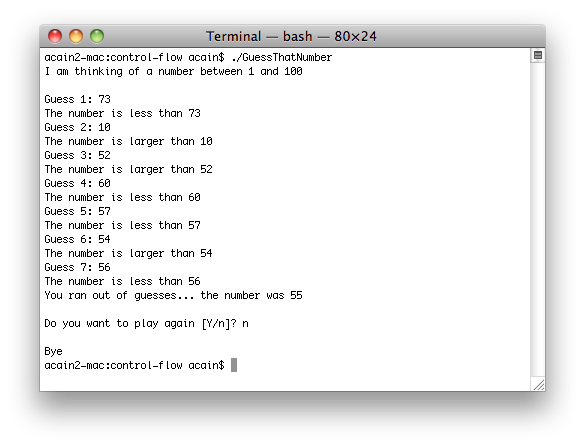
\includegraphics[width=0.5\textwidth]{./topics/control-flow/images/GuessThatNumber} 
   \caption[Guess That Number Terminal]{Guess that Number run from the Terminal}
   \label{fig:control-flow-guess-num}
\end{figure}

\clearpage
\subsection{Boolean Data} % (fold)
\label{sub:boolean_data}

The Boolean\footnote{Named after George Bool's Boolean logic.} Data Type is a \nameref{sub:type} used to represent \textbf{truth}. A Boolean value will either be \textbf{true} or \textbf{false}. These values are used extensively in the control flow statements to determine the action to perform.

\begin{figure}[h]
   \centering
   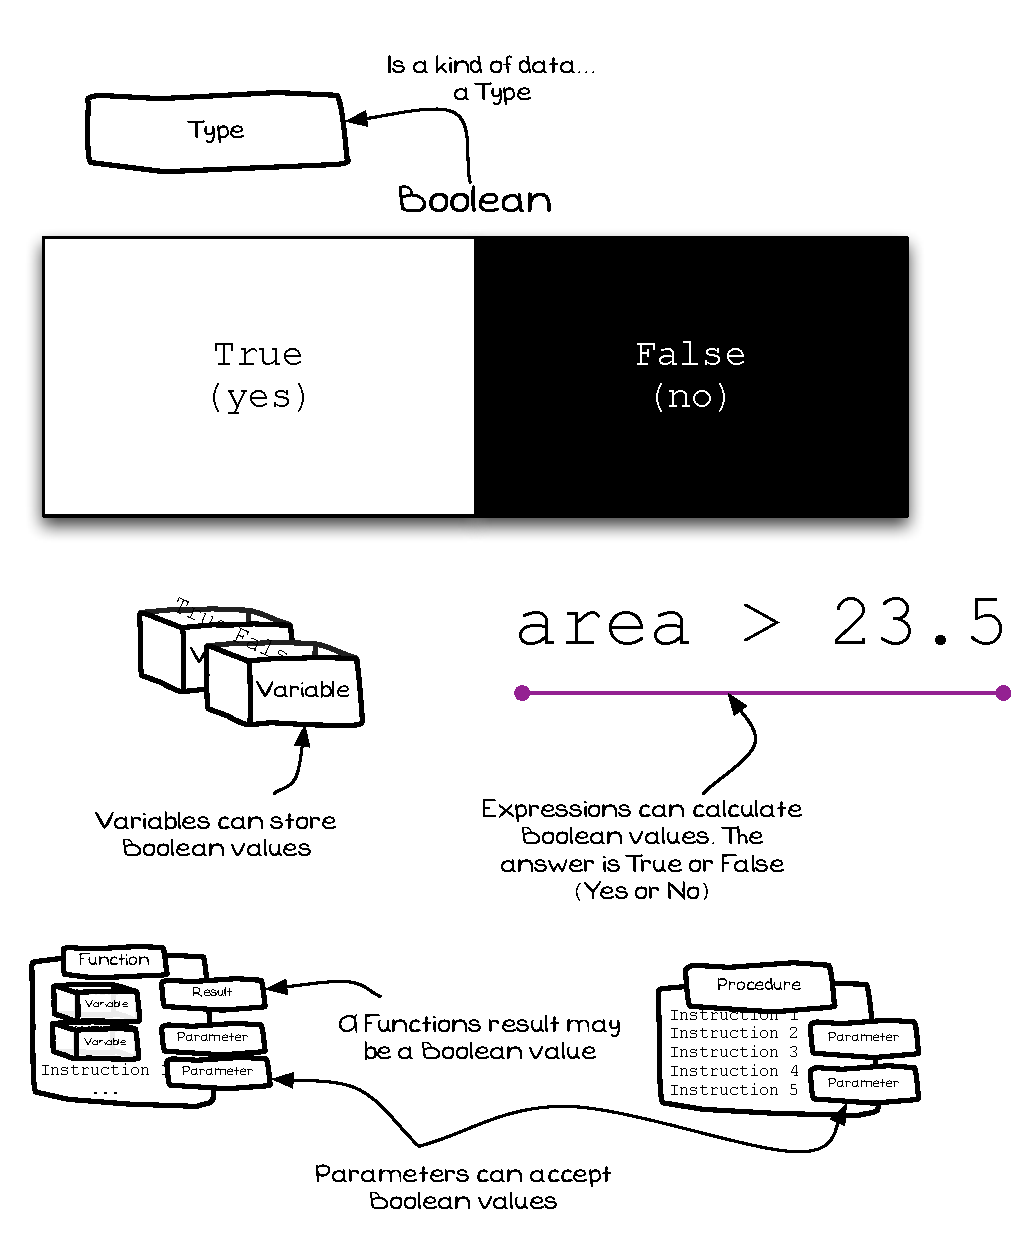
\includegraphics[width=0.8\textwidth]{./topics/control-flow/diagrams/BooleanData} 
   \caption{Boolean data represents truth}
   \label{fig:boolean-data}
\end{figure}

\mynote{
\begin{itemize}
  \item Boolean is an existing \textbf{artefact}, it is a \nameref{sub:type} that has been defined to represent truth values.
  \item A Boolean value is either \textbf{true} or \textbf{false}. You can also think of these as \emph{yes} and \emph{no}.
  \item Boolean values are used in most of the control flow statements.
  \item The Boolean type can be used in the same way as other types.
\end{itemize}
}
% subsection boolean_data (end)

\clearpage
\subsubsection{Comparisons} % (fold)
\label{sub:comparisons}

Comparisons are a common way of getting Boolean values in your code. These \nameref{sub:expression}s allow you to compare two values to check for a given condition. For example, the Expression shown in Figure \ref{fig:boolean-data} is asking if the \emph{value} in the \texttt{area} variable is larger than \texttt{23.5}. The result of this expression will be either \texttt{true} or \texttt{false} depending on the current value stored in \texttt{area}. Table \ref{tbl:bool-expr-sample} lists some example values for this expression, given different values stored in the \texttt{area} variable.

\begin{table}[h]
  \centering
  \begin{tabular}{|c|c|}
    \hline
    \textbf{Value in \texttt{area}} & \textbf{\texttt{area > 23.5}} \\
    \hline
    \texttt{73.2} & \texttt{true} \\
    \hline
    \texttt{-2.5} & \texttt{false} \\
    \hline
    \texttt{23.5} & \texttt{false} \\
    \hline
  \end{tabular}
  \caption{Example values for the expression \texttt{area > 23.5}}
  \label{tbl:bool-expr-sample}
\end{table}

Programming languages offer a range of different comparison operators. These typically include comparisons to check if values are the same or different, and to check if one value is larger or small than another. The different operators for C and Pascal are listed in Table \ref{tbl:comparisons}.

\begin{table}[h]
  \centering
  \begin{tabular}{|c|c|c|c|}
    \hline
     & \textbf{Description} & \textbf{C} & \textbf{Pascal} \\
    \hline
    \textbf{Equal} & Are the values the same? & \texttt{a == b} & \texttt{a = b} \\
    \hline
    \textbf{Not Equal} & Are the values different? & \texttt{a != b} & \texttt{a <> b} \\
    \hline
    \textbf{Larger Than} & Is the left value larger than the right? & \multicolumn{2}{c|}{\texttt{a > b}}  \\
    \hline
    \textbf{Less Than} & Is the left value smaller than the right? & \multicolumn{2}{c|}{\texttt{a < b}}  \\
    \hline
    \textbf{Larger Or Equal} & Is the left value equal or larger than the right? & \multicolumn{2}{c|}{\texttt{a >= b}}  \\
    \hline
    \textbf{Less Or Equal} & Is the left value smaller or equal to the right? & \multicolumn{2}{c|}{\texttt{a <= b}}  \\
    \hline
    
  \end{tabular}
  \caption{Comparison Operators}
  \label{tbl:comparisons}
\end{table}

\mynote{
\begin{itemize}
  \item Comparisons can only be performed between \textbf{two} values.
  \item The values on either side of the comparison are \nameref{sub:expression}s, allowing you to calculate the values being compared.
\end{itemize}
}

\csection{
C uses a double equal (\texttt{==}) for comparison as the single equals (\texttt{=}) is used for assignment.
}

% subsection comparisons (end)

\clearpage
\subsubsection{Logical Operators} % (fold)
\label{sub:logical_operators}

The comparison operators allow you to compare \emph{two} values. This is very useful, but in itself is incomplete. What, for example, do you do when you want to compare three or more values? While you are limited to two values with the comparison operators, there are other operators that allow you to \textbf{combine} Boolean expressions. This will enable you to combine together multiple Boolean values into a single Expression.

There are four main \emph{logical operators}: \textbf{and}, \textbf{or}, \textbf{xor}, and \textbf{not}. Each of these operators works on two Boolean values, combining them to give a new Boolean value. For example, the \emph{and} operator allows you to check if \emph{both} of the expressions are true. The expression \texttt{area > 0 and area < 10} will be true only when area is both larger than zero and less then ten.

\begin{figure}[h]
   \centering
   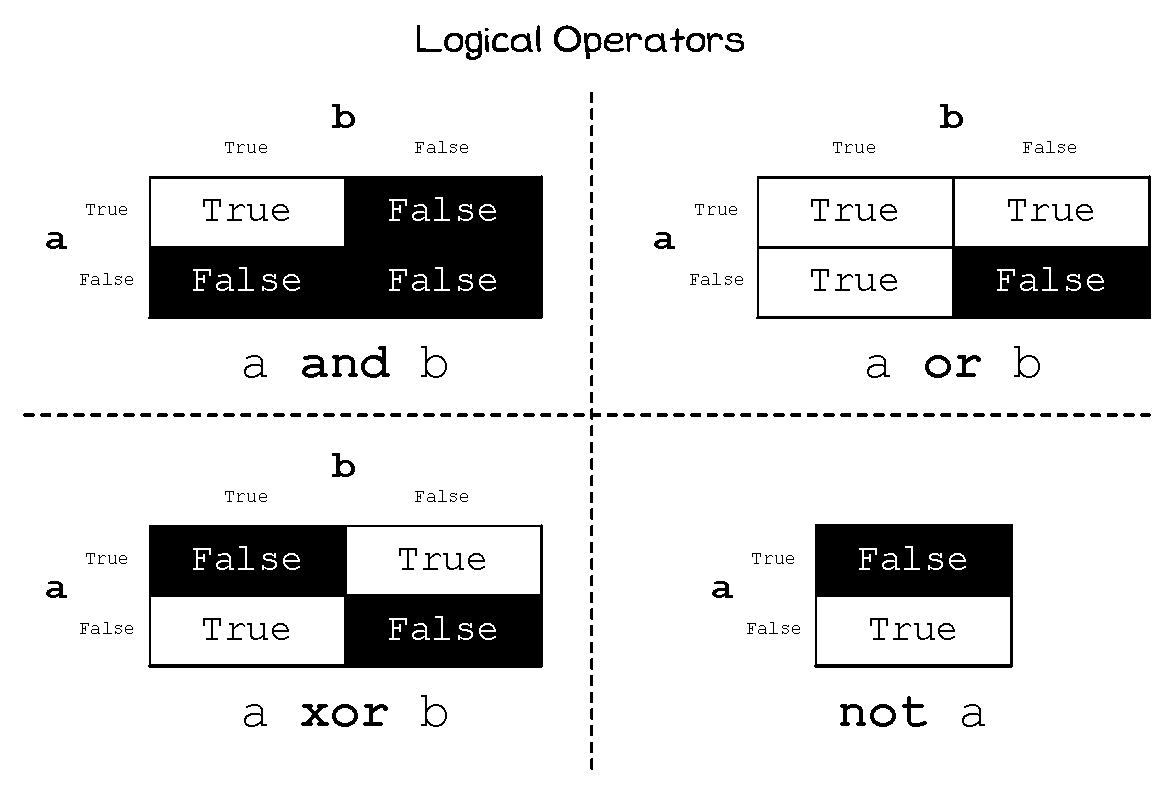
\includegraphics[width=0.7\textwidth]{./topics/control-flow/diagrams/LogicalOperators} 
   \caption{Logical Operators combine Boolean values}
   \label{fig:logical-operators}
\end{figure}

\begin{table}[h]
  \centering
  \begin{tabular}{|c|c|c|c|}
    \hline
     & \textbf{Description} & \textbf{C} & \textbf{Pascal} \\
    \hline
    \textbf{And} & Are both values True? & \texttt{a \&\& b} & \texttt{a and b} \\
    \hline
    \textbf{Or} & Is at least one value True? & \texttt{a || b} & \texttt{a or b} \\
    \hline
    \textbf{Xor} & Is one value True, and the other False? & \texttt{a \^{} b} & \texttt{a xor b} \\
    \hline
    \textbf{Not} & Is the value False? & \texttt{!a} & \texttt{not a}  \\
    \hline
  \end{tabular}
  \caption{Logical Operators}
  \label{tbl:logical-operators}
\end{table}

\begin{table}[h]
  \centering
  \begin{tabular}{|c|c|c|c|c|c|}
    \hline
    \multirow{2}{*}{area }& \multirow{2}{*}{\texttt{area > 0}} & \multirow{2}{*}{\texttt{area < 10}} & \multicolumn{3}{c|}{\texttt{area > 0 {\textbf{\ldots}} area < 10}} \\
    \cline{4-6}
     &  &  & \textbf{and} & \textbf{or} & \textbf{xor} \\
    \hline
    \texttt{\textbf{5}} & True & True & True & True & False \\
    \hline
    \texttt{\textbf{27}} & True & False & False & True & True \\
    \hline
    \texttt{\textbf{0}} & False & True & False & True & True \\
    \hline
  \end{tabular}
  \caption{Example Logical Expressions}
  \label{tbl:example_logical_expr}
\end{table}

\mynote{
\begin{itemize}
  \item Table \ref{tbl:example_logical_expr} has some example expressions.
  \item The tables in Figure \ref{fig:logical-operators} show the values of the different logical operators. These are known as \textbf{Truth Tables}.
  \item Table \ref{tbl:logical-operators} outlines the different logical operators, and how they are coded in C and Pascal.
\end{itemize}
}



% subsection boolean_logic (end)

\subsection{Branching} % (fold)
\label{sub:branching}

There are two main ways of controlling the sequence of actions in a program. The first of these is called \textbf{branching}, or \textbf{selection}. Branching allows you to get the computer to take one of a number of paths based on the value of a \emph{condition}.

\begin{figure}[h]
   \centering
   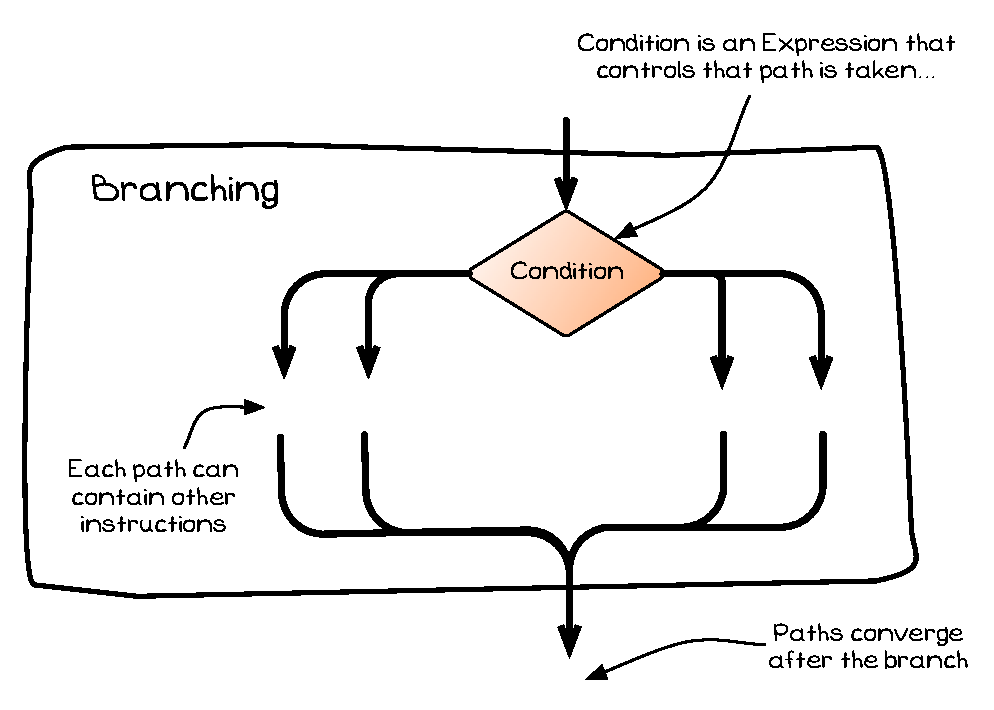
\includegraphics[width=0.8\textwidth]{./topics/control-flow/diagrams/Branching} 
   \caption{Branching commands the computer to take one of a number of possible paths}
   \label{fig:branching}
\end{figure}

\mynote{
\begin{itemize}
  \item Branching is a kind of \textbf{action}. You can command the computer to take of a number of paths.
  \item A branch has a \textbf{condition} that is evaluated, and based on the condition the computer takes one path.
  \item The branch is the act of choosing the path, when its command is performed the computer evaluates the condition and then moves to the instructions in the indicated path.
  \item Languages usually offer two kinds of branching statements:
  \begin{itemize}
    \item \nameref{sub:if_statement} to select between two paths based on a Boolean expression.
    \item \nameref{sub:case_statement}  to select a path based on an ordinal\footnote{Integers and Characters are ordinal values. Ordinal values have a defined sequence, so it is possible to say which value comes next in the sequence. Integers are Ordinal as you can say that the number after 1 is 2. Real numbers are not ordinal as you cannot say which value comes next in the sequence.} value.
  \end{itemize}
  \item The Branch will have one entry point, and one exit point. This feature allows you to combine statements together like building blocks. This idea comes from the principles of \textbf{Structured Programming}, where each component in the code should have a single entry and exit point.
\end{itemize}
}


% subsection branching (end)
\clearpage
\subsubsection{If Statement} % (fold)
\label{sub:if_statement}

The if statement is the most frequently used branching statement. It allows you to selectively run code based on the value of a Boolean expression (the condition). The if statement has an optional \emph{else} branch that is executed when the condition is false.

\begin{figure}[h]
   \centering
   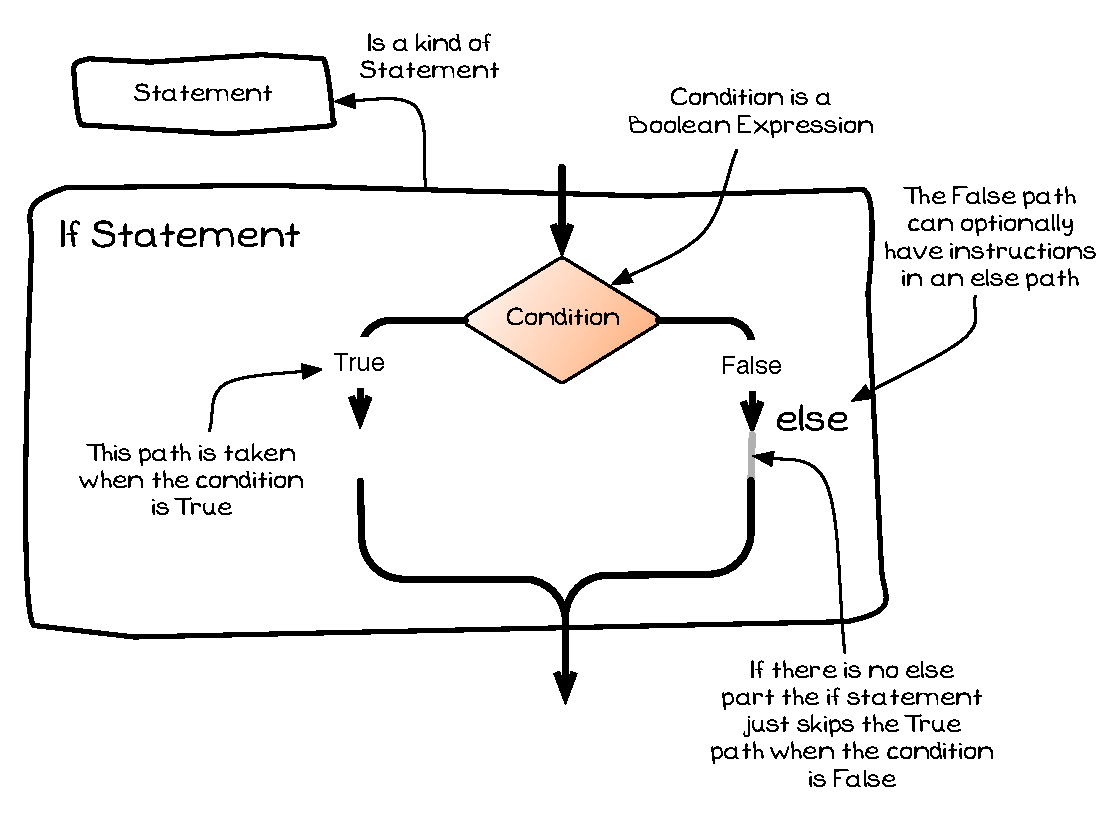
\includegraphics[width=\textwidth]{./topics/control-flow/diagrams/IfStatement} 
   \caption{If statement lets you selectively run a branch of code}
   \label{fig:branching-if-statement}
\end{figure}

\mynote{
\begin{itemize}
  \item An if statement is an \textbf{action}. It allows you to command the computer to select a path based on a Boolean expression.
  \item The if statement has two branches, one that is taken when the condition is True, the other when it is False.
  \item The False branch may \emph{optionally} have instructions that are carried out when the condition is False. 
  \item If there are no instructions you want performed when the condition is False you do not need to include an else branch, and the if statement will just skip the True branch when the condition is False.
  \item The if statement has one entry point, two paths, and then one exit point.
\end{itemize}
}


% subsection if_statement (end)
\clearpage
\subsubsection{Case Statement} % (fold)
\label{sub:case_statement}

The case statement is the second kind of branching statement. This allows you to create paths that execute based on matching a value from an expression. This allows one case statement to handle many alternative paths.

\begin{figure}[h]
   \centering
   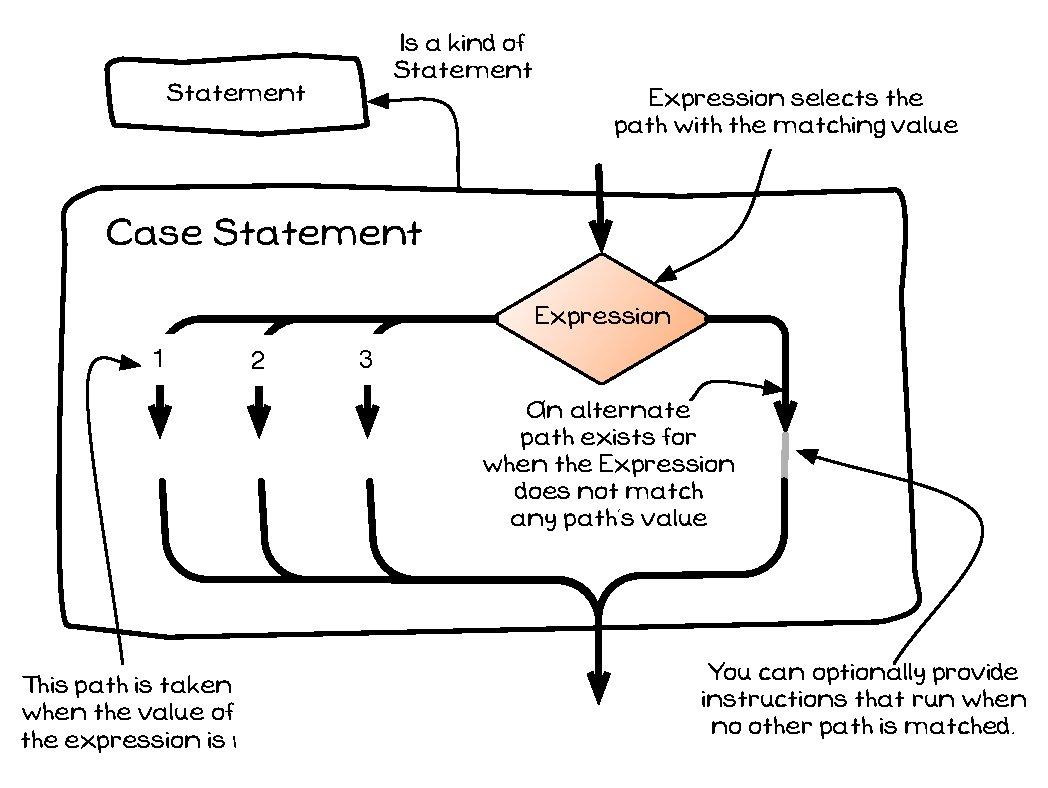
\includegraphics[width=\textwidth]{./topics/control-flow/diagrams/CaseStatement} 
   \caption{Case statement selectively runs multiple branches of code}
   \label{fig:branching-case-statement}
\end{figure}

\mynote{
\begin{itemize}
  \item The case statement is a kind of \textbf{action}. It allows you to command the computer to select a path based upon the value of an expression.
  \item Each path within the Case Statement has a value. When the computer executes the case statement the path values are used to determine which path will be taken.
  \item In C and Pascal the Case Statement only works with Ordinal Values. This limits you to using Character or Integer values within the Case Statement's Expression.
  \item The Case Statement has one entry point, multiple paths, and then one exit point.
\end{itemize}
}

% section case_statement (end)

\clearpage
\subsection{Looping} % (fold)
\label{sub:looping}

There are two main ways of controlling the sequence of actions in a program. The first was \textbf{branching}, the second is called \textbf{looping}, or \textbf{repetition}. The language's looping statements allow you to have actions repeated.

\begin{figure}[h]
   \centering
   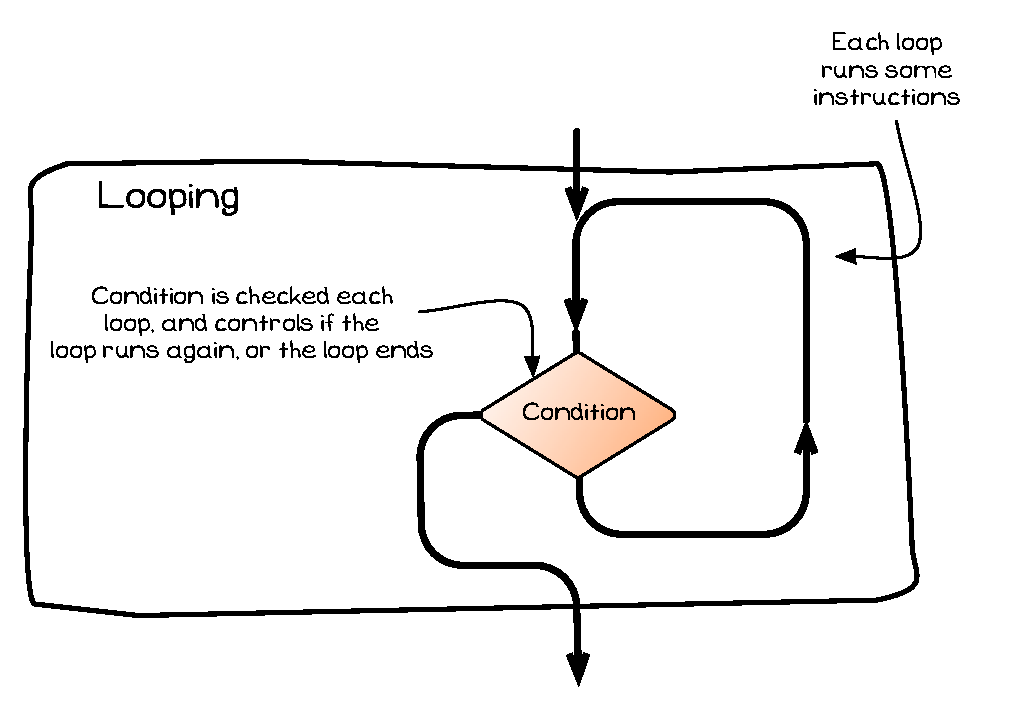
\includegraphics[width=0.9\textwidth]{./topics/control-flow/diagrams/Looping} 
   \caption{Looping commands the computer to repeat a path}
   \label{fig:looping}
\end{figure}

\mynote{
\begin{itemize}
  \item Looping is a kind of \textbf{action}. You can command the computer to repeat the steps within a path.
  \item A number of steps are performed each loop:
  \begin{itemize}
    \item The instructions within the loop are executed.
    \item The \emph{condition} is checked, and the instructions are either run again or the loop ends.
  \end{itemize}
  \item The \emph{condition} may be checked before or after the instructions are executed, giving two kinds of loops:
  \begin{itemize}
    \item \nameref{sub:pre_test_loop}: Repeats instructions 0 or more times.
    \item \nameref{sub:post_test_loop}: Repeats instructions 1 or more times.
  \end{itemize}
  \item As with Branching, the Looping Statements have a single entry and a single exit in keeping with the principles of \textbf{Structured Programming}.
\end{itemize}
}


% subsection looping (end)
\clearpage
\subsubsection{Pre-Test Loop} % (fold)
\label{sub:pre_test_loop}

The Pre-Test Loop is a looping statement that allows code to be run 0 or times. The loop checks the condition at the start, and if the condition is True the loop's body is executed. At the end of the loops body the computer jumps back to the condition, checking it again to determine if the loop's body should execute again. If the condition is False when it is checked the loop jumps ends, and control jumps to the next statement in the code.

\begin{figure}[h]
   \centering
   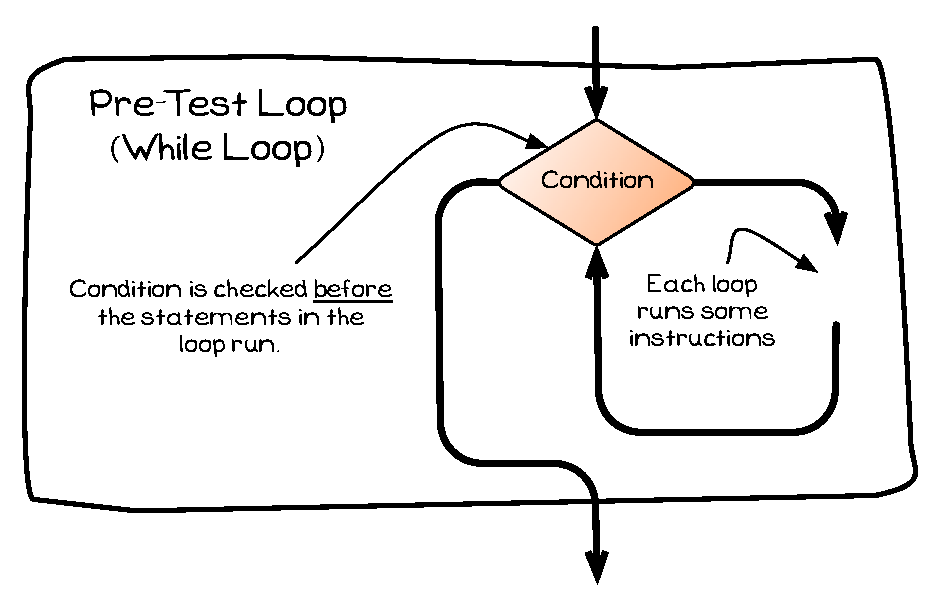
\includegraphics[width=\textwidth]{./topics/control-flow/diagrams/PreTestLoop} 
   \caption{The Pre-Test Loop checks the condition, then runs the loop's body}
   \label{fig:looping-pre-test}
\end{figure}

\mynote{
\begin{itemize}
  \item A pre-test loop is an \textbf{action}, creating a loop in the code's sequence of instructions.
  \item The standard pre-test loop is the \textbf{while statement}.
  \item A pre-test loop allows instructions to be run 0 or more times.
  \item The condition is checked when the loop's code is entered, and it is checked again at the end of each loop.
\end{itemize}
}


% subsection post_test_loop (end)
\clearpage
\subsubsection{Post-Test Loop} % (fold)
\label{sub:post_test_loop}

The Post-Test Loop is a looping statement that allows code to be run 1 or times. The post-test loop places the condition after the body of the loop. This means that the first time through the body of the loop must execute before the condition is checked. When it gets to the end of the body, the loop's condition is checked and the computer either jumps back to the start of the loop to repeat the body, or the loop ends and control flows on to the next statement in the code.

There are two common variants for the post-test loop: \texttt{\textbf{do...while}} and \texttt{\textbf{repeat...until}}. These work in the same way, in that they test the condition after the loop body, but the conditions they use will be different. The \textbf{\texttt{do...while}} loop repeats the body of the loop when its condition is \textbf{true}, \textbf{\texttt{repeat...until}} repeats the body of the loop when its condition is \textbf{false}. When implementing a post-test loop you must make sure that the condition you use matches the kind of loop supported by your language.

\begin{figure}[h]
   \centering
   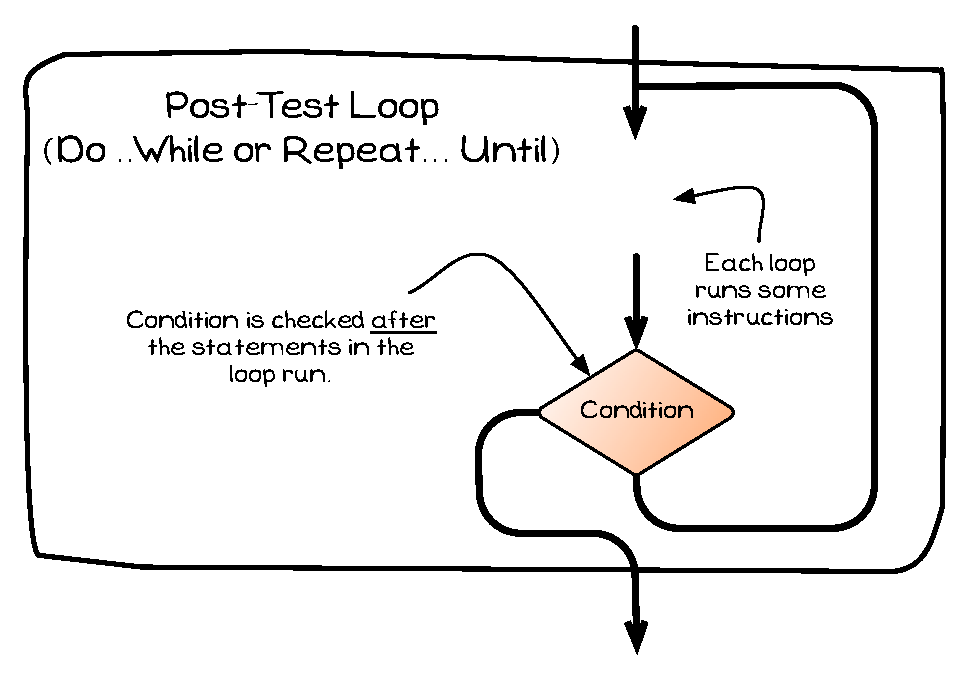
\includegraphics[width=0.9\textwidth]{./topics/control-flow/diagrams/PostTestLoop} 
   \caption{The Post-Test Loop runs the loops body, then checks the condition}
   \label{fig:looping-post-test}
\end{figure}

\mynote{
\begin{itemize}
  \item A post-test loop is an \textbf{action}, creating a loop in the code's sequence of instructions.
  \item A post-test loop allows instructions to be run 1 or more times.
  \item The condition is checked after the loop's body is executed, with control jumping back to the start if needed.
\end{itemize}
}

\csection{C includes support for the \textbf{\texttt{do...while}} loop.}
\passection{Pascal includes support for the \textbf{\texttt{repeat...until}} loop.}

% subsection post_test_loop (end)

\clearpage
\subsection{Jumping} % (fold)
\label{sub:jump}

The jump statements allow you to alter the sequence of instructions in the code, getting the computer to jump to another instruction.

\begin{figure}[h]
   \centering
   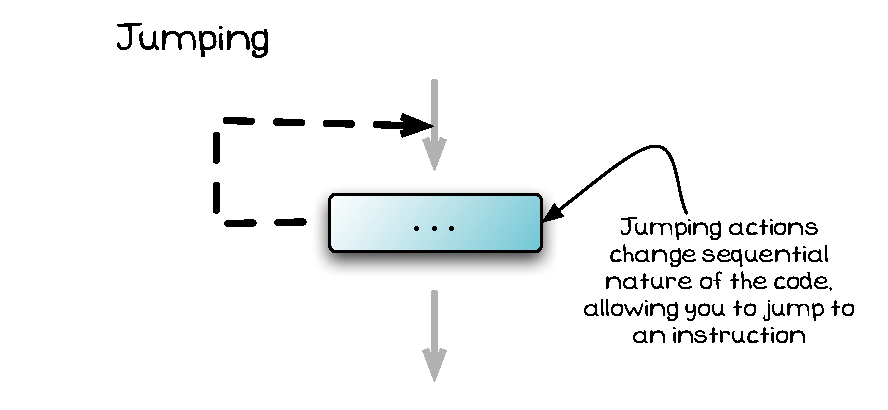
\includegraphics[width=\textwidth]{./topics/control-flow/diagrams/JumpStatements} 
   \caption{Jump Statements cause control to jump to another location in the code}
   \label{fig:looping-jump-statements}
\end{figure}

\mynote{
\begin{itemize}
  \item The jump statements are \textbf{actions}, they allow you to alter the standard sequence of the instructions and have the computer jump to a another location in the instructions.
  \item \textbf{Structured Programming} was proposed as a means of providing order and structure to the control flow through the code. These jump statements complicate this sequential flow, but in some cases they are able to simplify code.
  \item Structured jump statements allow you to control the sequence of actions related to a \nameref{sub:looping} statement, a \nameref{sub:function}, or a \nameref{sub:procedure}. These work the looping and procedural structures used in structured programming.
  \item Unstructured jump statements allow you to jump to any instruction within the code. You need to be aware that these statements exist, but they should not be used.
\end{itemize}
}

% subsection jump_statements (end)
\clearpage
\subsubsection{Break} % (fold)
\label{sub:break}

The break statement is used to jump out of the current loop, in effect terminating the loop early. This is useful for ending the current loop, skipping all future cycles.

\begin{figure}[h]
   \centering
   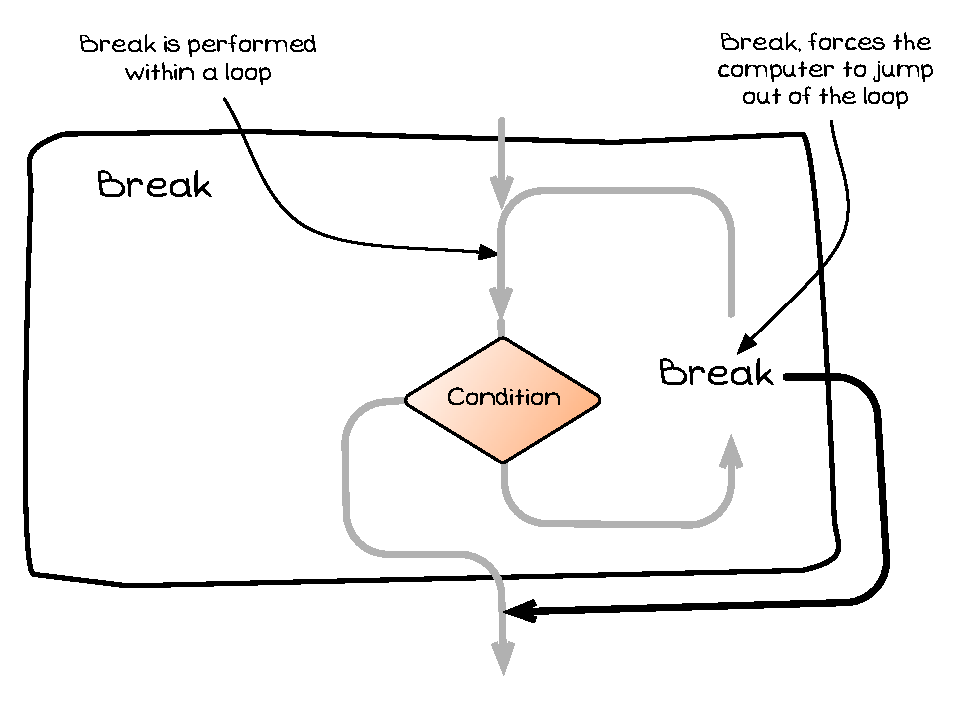
\includegraphics[width=\textwidth]{./topics/control-flow/diagrams/Break} 
   \caption{The Break Statement allows you to end a loop early}
   \label{fig:break}
\end{figure}

\mynote{
\begin{itemize}
  \item The break statement is an \textbf{action}, allowing you to jump to the end of the current loop.
  \item The break statement should be coded within an \nameref{sub:branching} statement that checks if the loop should terminate early.
\end{itemize}
}


% subsection break (end)
\clearpage
\subsubsection{Continue} % (fold)
\label{sub:continue}

The continue statement is used to jump to the condition of the current loop. This is useful for skipping the processing of the current loop, but to allow the loop to continue for the next cycle.

\begin{figure}[h]
   \centering
   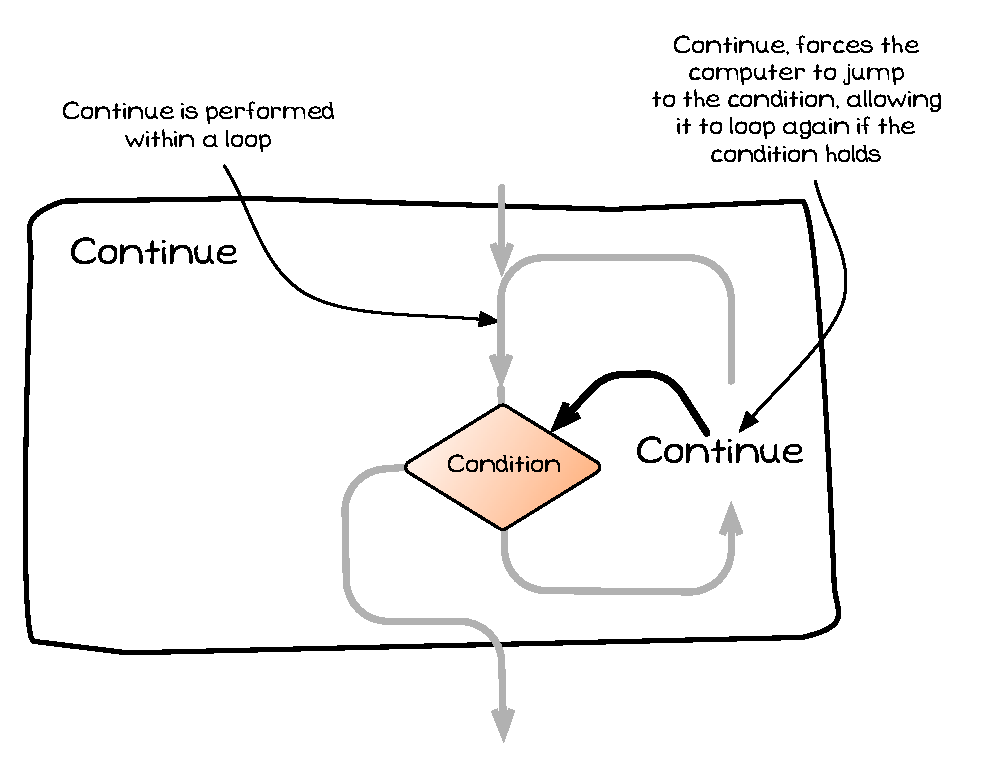
\includegraphics[width=\textwidth]{./topics/control-flow/diagrams/Continue} 
   \caption{The continue Statement allows you to jump to the condition, skipping the remainder of the code in the loop but allowing the loop to continue}
   \label{fig:continue}
\end{figure}

\mynote{
\begin{itemize}
  \item The continue statement is an \textbf{action}, allowing you to jump to the condition of the current loop.
  \item The continue statement should be coded within an \nameref{sub:branching} statement that checks if the loop should skip processing of the current cycle.
\end{itemize}
}


% subsection break (end)
\clearpage
\subsubsection{Exit} % (fold)
\label{sub:exit}

The exit statement, or the return in C, ends the current \nameref{sub:function} or \nameref{sub:procedure}. This is useful for skipping the rest of the processing of the Function or Procedure, exiting it early and returning to the calling code. 

\begin{figure}[h]
   \centering
   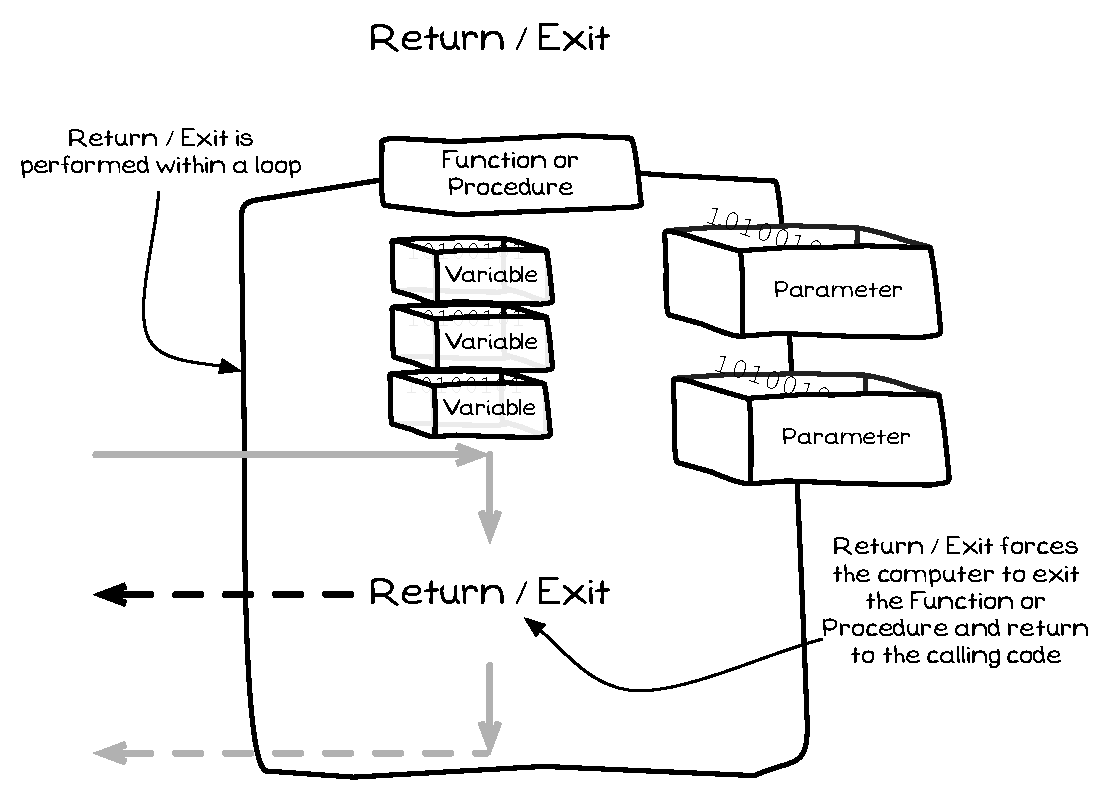
\includegraphics[width=\textwidth]{./topics/control-flow/diagrams/Return} 
   \caption{Exit ends the current Function or Procedure}
   \label{fig:exit}
\end{figure}

\mynote{
\begin{itemize}
  \item Exit is an \textbf{action}, allowing you to jump out of the current Function or Procedure, and return to the calling code.
  \item The Exit should be coded within a \nameref{sub:branching} statement that checks if the Function or Procedure should end.
\end{itemize}
}

\csection{C's version of the exit statement is the \nameref{sub:return_statement}. The return statement also provides the value that will be returned when exiting from a Function. As this sets the value to be returned you must have a return statement as the last action within a Function.}

% subsection return_or_exit_statement (end)
\clearpage
\subsubsection{Goto} % (fold)
\label{sub:goto}

The last jump statement is the goto statement. This is an unstructured jump, allowing you to jump anywhere in the code. Structured Programming principles called for the abolition of the goto statement. This is a statement you need to be aware of, but not one that should be used.

\begin{figure}[h]
   \centering
   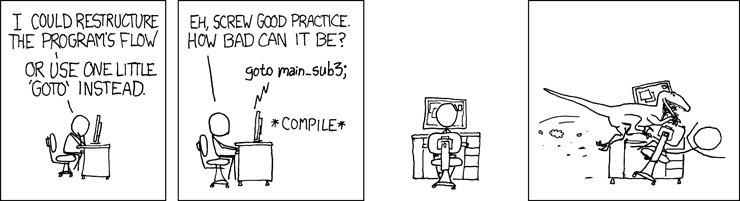
\includegraphics[width=\textwidth]{./topics/control-flow/images/goto} 
   \caption{The dangers of using goto, from \url{http://xkcd.com/292/}}
   \label{fig:goto}
\end{figure}

\mynote{
\begin{itemize}
  \item Goto is an action that allows you to jump to another instruction and continue from there.
  \item You need to be aware of the goto statement, but you should not use it.
\end{itemize}
}

% subsection goto (end)


\clearpage
\subsection{Compound Statement} % (fold)
\label{sub:compound_statement}

\nameref{sub:branching} and \nameref{sub:looping} statements need to be able to include a number of instructions within their paths. Often languages will manage this by indicating that only a \emph{single} statement can be included in any of these paths, and then include the ability to code multiple statements in a \emph{single compound statement}.

\begin{figure}[h]
   \centering
   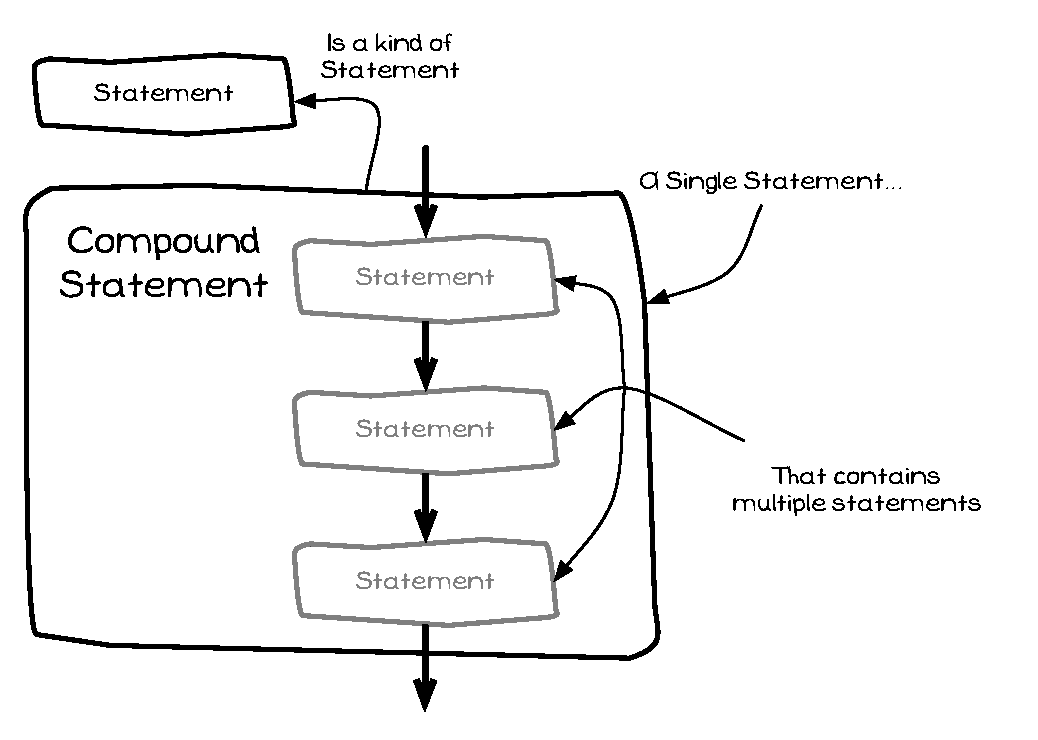
\includegraphics[width=\textwidth]{./topics/control-flow/diagrams/CompoundStatement} 
   \caption{A Compound Statement is a Statement that can contain other Statements}
   \label{fig:branching-compound-statement}
\end{figure}

\mynote{
\begin{itemize}
  \item A Compound Statement is a way of grouping \textbf{action}s, allowing you to create a single statement that contains multiple statements.
  \item Compound Statements are useful when combined with \nameref{sub:branching} and \nameref{sub:looping} Statements. Allowing you to put multiple statements within a path.
\end{itemize}
}

% subsection compound_statements (end)
\clearpage
\subsection{Statement (Simple and Structured)} % (fold)
\label{sub:statement_with_loops_}

Statements are the actions that we can get the computer to perform.  

\begin{figure}[h]
   \centering
   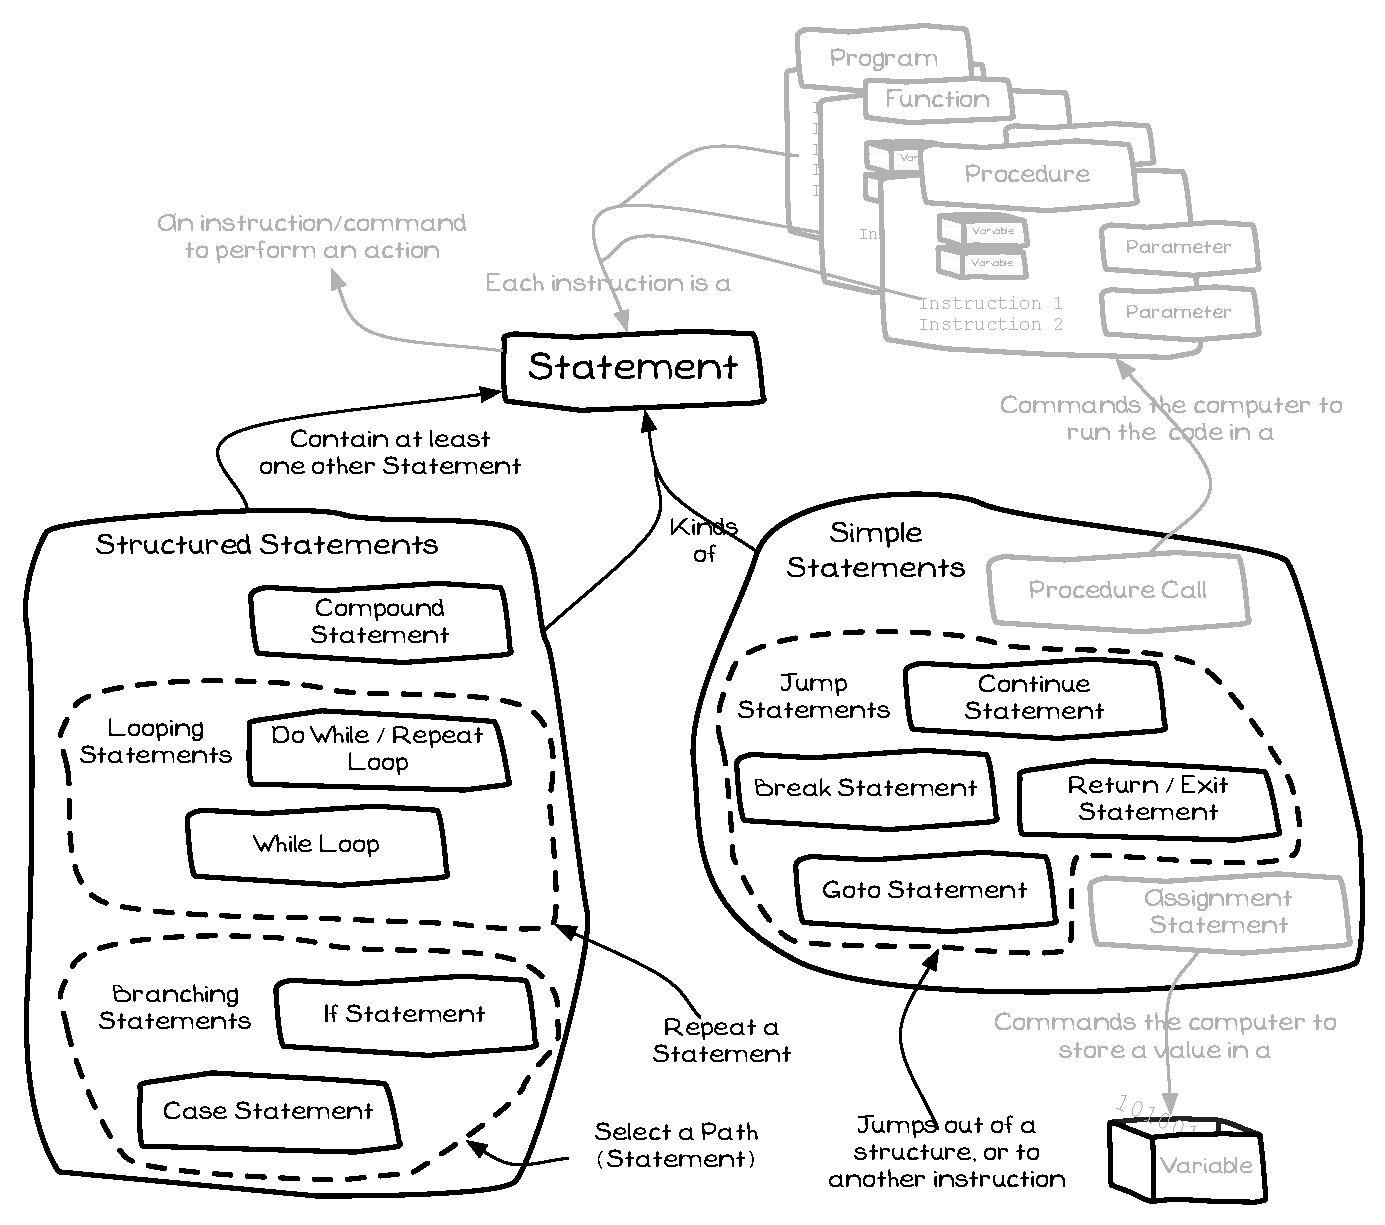
\includegraphics[width=0.88\textwidth]{./topics/control-flow/diagrams/Statement}
   \caption{A Statement may also be a Looping or Jumping Statement}
   \label{fig:looping-statement}
\end{figure}

\mynote{
\begin{itemize}
  \item Statement is the \textbf{term} given to the instructions in code.
  \item \textbf{Simple Statements} that perform an action. The actions you can perform are:
  \begin{itemize}
    \item \nameref{sub:procedure call} used to run the code in a Procedure.
    \item \nameref{sub:assignment_statement} used to calculate a value and store it in a Variable.
    \item Jump Statements allow you to affect which instruction will be performed next. This includes:
    \begin{itemize}
      \item \nameref{sub:break}: to jump out of a \nameref{sub:looping} Statement.
      \item \nameref{sub:continue}: jumps to the condition in a Looping Statement.
      \item \nameref{sub:exit}: (return in C) to end the current Function or Procedure.
      \item \nameref{sub:goto}: the unstructured jump\footnote{Often resulting in death by Raptor.} to an arbitrary location in the code.
    \end{itemize}
  \end{itemize}
  \item \textbf{Structured Statements} contain statements and control the flow of execution:
  \begin{itemize}
    \item \nameref{sub:looping} Statements: that repeat a statement a number of times.
    \begin{itemize}
      \item \nameref{sub:pre_test_loop}: Test condition before the body, repeating \textbf{0 to many} times.
      \item \nameref{sub:post_test_loop}: Test condition after the body, repeating \textbf{1 to many} times.
    \end{itemize}
    \item \nameref{sub:branching} Statement: that select from a number of optional statements.
    \begin{itemize}
      \item \nameref{sub:if_statement}: Branch based on a \nameref{sub:boolean_data} Expression (2 paths).
      \item \nameref{sub:case_statement}: Branch based on an Ordinal Expression (\emph{n} paths).
    \end{itemize}
  \end{itemize}
\end{itemize}
}


% subsection statement_with_loops_ (end)

\clearpage
\subsection{Summary} % (fold)
\label{sub:control_flow_summary}

This section has introduced a number of new actions that you can use in your code to create more dynamic programs. 

\begin{figure}[h]
   \centering
   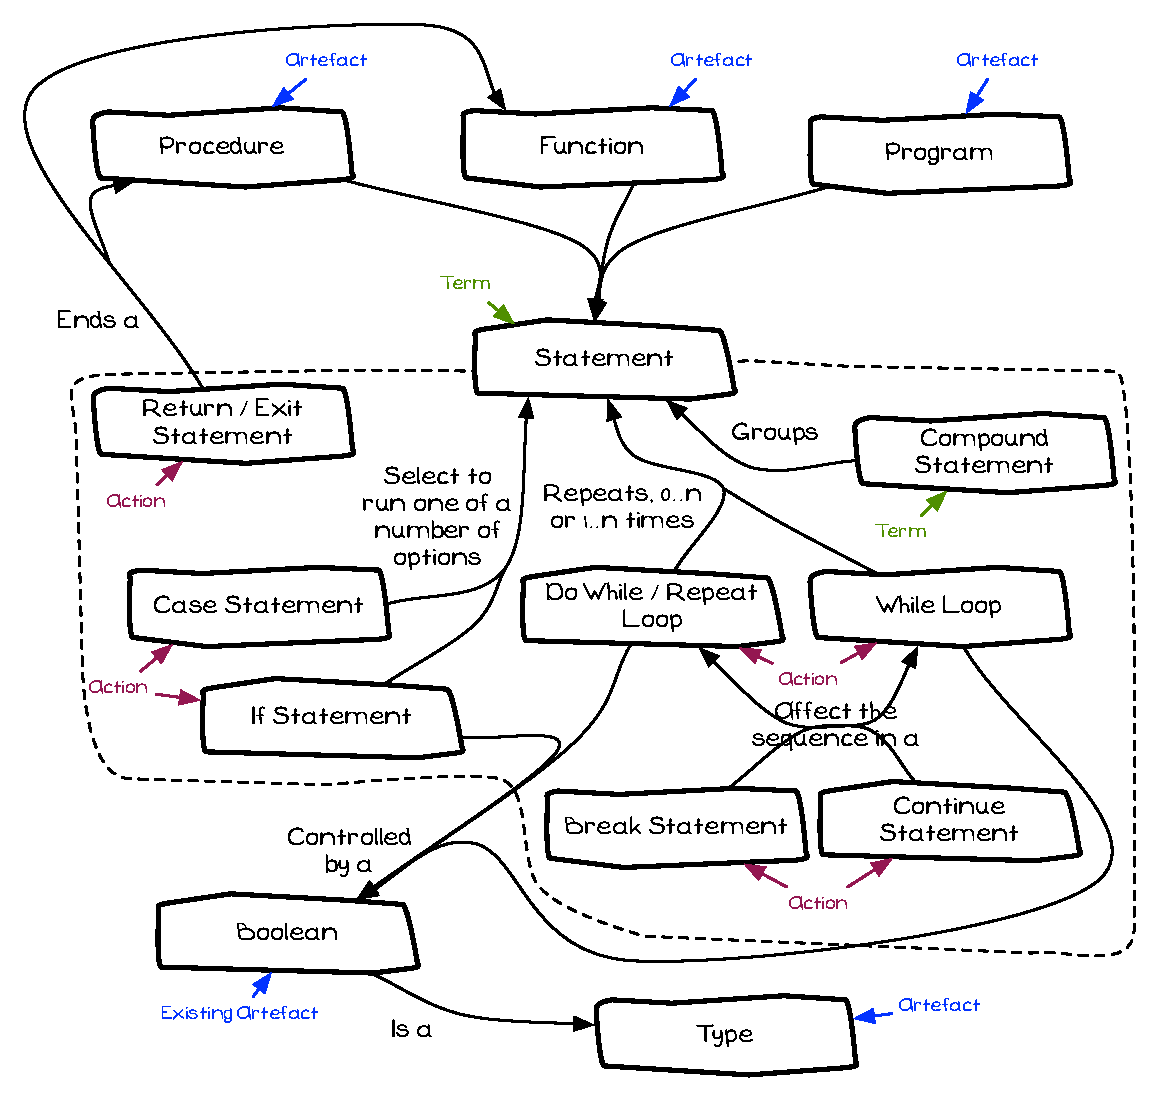
\includegraphics[width=\textwidth]{./topics/control-flow/diagrams/Summary} 
   \caption[Chapter Concepts]{Key Concepts introduced in this Chapter}
   \label{fig:control-flow-summary}
\end{figure}

\mynote{
\begin{itemize}
  \item \textbf{Artefacts} are things you can \emph{create} and \emph{use}.
  \item \textbf{Terms} are things you need to \emph{understand}.
  \item \textbf{Actions} are things you can \emph{command} the computer to perform.
\end{itemize}
}

% subsection summary (end)
% section control-flow_concepts (end)

% ======================
% = Using Control Flow =
% ======================
\clearpage
\section{Using these Concepts} % (fold)
\label{sec:control_flow_using_these_concepts}

The Control Flow Statements enable you to alter the purely sequential order in which instructions are performed. Using these Statements you can have the computer select a path to follow, or jump back and repeat statements a number of times. These capabilities make it possible to create programs that react to the data they receive, giving more interactive results than were possible before.

\subsection{Designing Guess that Number} % (fold)
\label{sub:designing_guess_that_number}

Table \ref{tbl:control-flow-prog} contains a description of the next program we are going to design. This program plays a small guessing game called \emph{Guess that Number}. In this game the computer will think of a target number between 1 and 100. The user then has 7 guesses to determine the target number's value. At each guess the computer outputs a message to indicate if the target number is greater than, less than, or equal to the user's guess.

\begin{table}[h]
\centering
\begin{tabular}{l|p{10cm}}
  \hline
  \multicolumn{2}{c}{\textbf{Program Description}} \\
  \hline
  \textbf{Name} & \emph{Guess that Number} \\
  \\
  \textbf{Description} & A simple guessing game where the computer `thinks' of a number between 1 and 100, and the user has seven guesses to guess it. With each guess the computer indicates if the number it is thinking of is less than, or greater than the user's guess. If the user runs out of guesses they are shown the answer, and that round ends. After each round the user has the option to play again, or to quit the program.\\
  \hline
\end{tabular}
\caption{Description of the Guess That Number program.}
\label{tbl:control-flow-prog}
\end{table}

As before, the process to design and implement this program will follow a number of steps:
\begin{enumerate}
  \item Understand the problem, and get some ideas on the tasks that need to be performed.
  \item Choose the artefacts we will create and use
  \item Design the control flow for the procedural\footnote{The program, and any Functions and Procedures.} artefacts
  \item Map these artefacts to code
  \item Compile and run the program
\end{enumerate}

The new step in this process will involve designing the flow of the instructions within the program, and the Functions and Procedures that need to be created. Previously each artefact had a sequential flow of instructions, the introduction of the control flow statements has made it possible to add branches and loops to this sequence. The order of these actions needs to be considered for each sequence of instructions in your code.

% subsection designing_guess_that_number (end)

\clearpage
\subsection{Understanding Guess that Number} % (fold)
\label{sub:understanding_guess_that_number}

Guess that Number is a relatively common game involving one player choosing a number, and the other trying to guess it. Each guess is followed by an indication of whether the guess was less than or larger than the target number. The game continues until the player guesses the target number.

The data for this program will be relatively simple. The code will need to keep track of the current \textbf{target number} which will be an integer. The player will be able to enter a \textbf{guess}, also an integer. These two numbers represent the data model for the game. It is a game that involves a \emph{target number} and \emph{guess}.

The actions within the program involve \textbf{playing the game}, and \textbf{performing a guess}. Playing the game is the process of performing guesses until the player finally guesses the target number. This version of the game will only allow the player to have seven guesses, so this will need to be a part of this code in the program. The process of performing a guess will involve getting the user's guess, and giving them feedback indicating if they guessed the target number, of if they were larger than, or less than the target.

% subsubsection understanding_guess_that_number (end)

\subsection{Choosing Artefacts for Guess that Number} % (fold)
\label{sub:choosing_artefacts_for_guess_that_number}

Software design is all about \textbf{abstraction}. This is the process of determining the essential features of the problem and modelling that in the artefacts that you create in your code. When designing the artefacts that will make up your code you need to think about problem, and try to create artefacts in your code that represent the actions and data you imagine when thinking about the problem.

Our understanding of the Guess that Number game indicates that there are two processes that need to be performed within the program: \textbf{play game} and \textbf{perform guess}. These two processes can be coded as either Functions or Procedures in the program's code. The \texttt{Play Game} code can be implemented as a \nameref{sub:procedure}. It will be responsible for running the process of the game, starting with telling the user it has `thought of a number', through to coordinating the guesses, ending only when the user gets the answer of runs out of guesses.

\texttt{Perform Guess}, on the other hand, will need to be a \nameref{sub:function} as it must return back a \nameref{sub:boolean_data} value indicating if the user has guessed the number. The code in \texttt{Perform Guess} will be responsible for asking the user to enter a guess, and then giving them the feedback on their guess. As this has the details of the guess, its result is needed to allow \texttt{Play Game} to determine if the user has guessed the number.

The \texttt{Perform Guess} code will also need to accept parameters to tell it what the current \texttt{target} value is. This data will exist within the \texttt{Play Game} code, so it will need a mechanism to pass that code to \texttt{Perform Guess}. A \nameref{sub:parameter} is needed in \texttt{Perform Guess} to accept \texttt{target} will enable this. 

A nicety may be to allow tell the user which guess they are up to. Once again, this information is stored in \texttt{Play Game}, so a second parameter can be added to allow \texttt{Play Game} to pass in the \texttt{guess number} along with the \texttt{target} number.

In addition to these it has been decided to add a \texttt{Print Line} procedure to display a line of `-' characters. This will be displayed at the end of the game before the user is asked if they want to play again. A \texttt{length} parameter will enable the caller to indicate how many of these characters are printed on the line.

The Structure Chart showing these artefacts is shown in Figure \ref{fig:guess-game-structure}, and the Sequence Diagram is shown in Figure \ref{fig:guess-game-seq}. Notice that there is some relationship here between the artefacts that we are creating and the steps in the game itself. The earlier it is to see the relationship between these artefacts and the problem, the better job you have done abstracting your solution.

\begin{figure}[htbp]
   \centering
   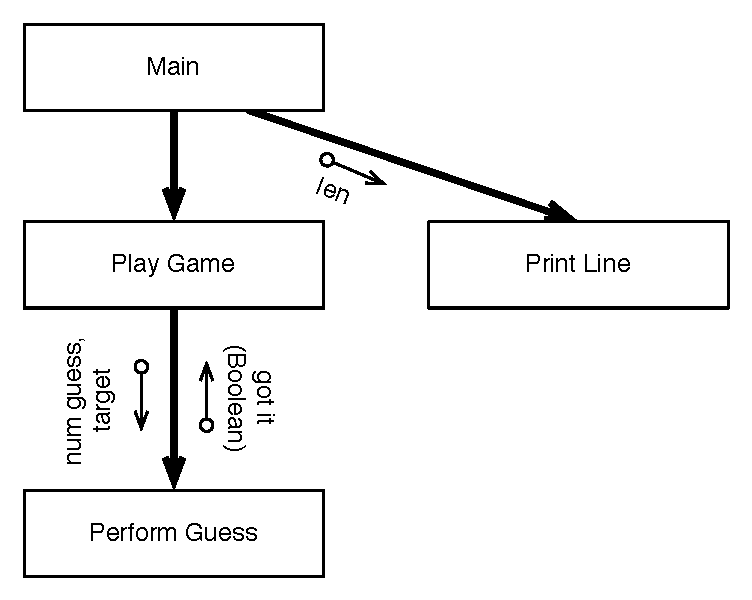
\includegraphics[width=0.6\textwidth]{./topics/control-flow/diagrams/GuessThatNumStructure} 
   \caption{Structure Chart for the Guess that Number Program}
   \label{fig:guess-game-structure}
\end{figure}

\begin{figure}[htbp]
   \centering
   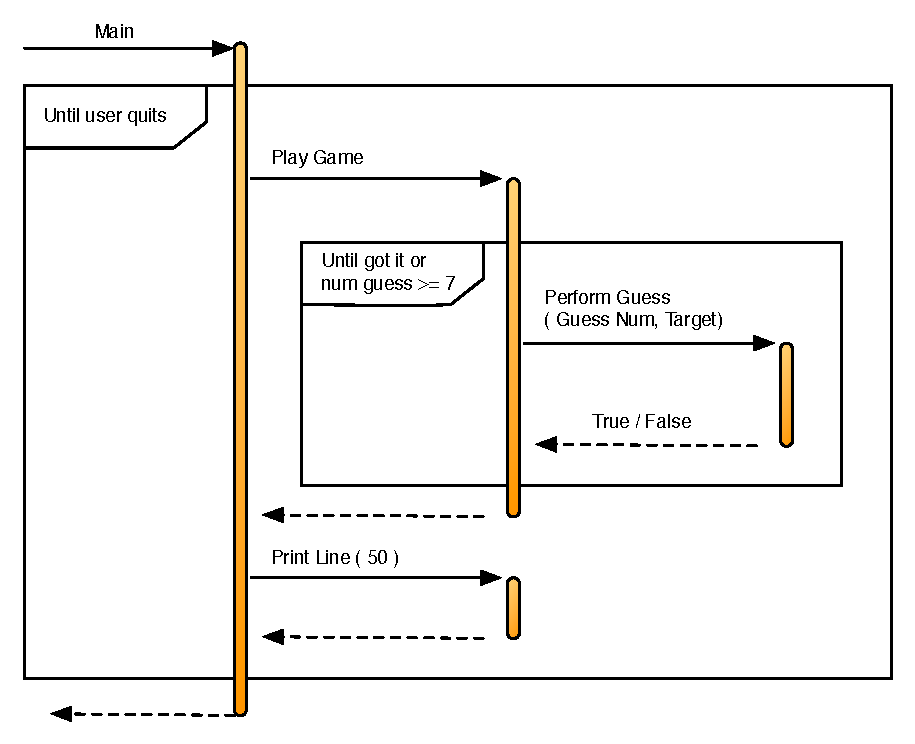
\includegraphics[width=\textwidth]{./topics/control-flow/diagrams/GuessThatNumSeq} 
   \caption{Sequence Diagram for the Guess that Number Program}
   \label{fig:guess-game-seq}
\end{figure}
% subsection choosing_artefacts_for_guess_that_number (end)

\clearpage
\subsection{Designing Control Flow for Perform Guess} % (fold)
\label{sub:designing_control_flow_for_perform_guess}

Having chosen the artefacts to build, the next step is to design the control flow that will enable these Functions and Procedures, and the program itself, to achieve their goals. Each has a responsibility that it must meet in order for the overall solution to work. 

This section will go through designing the logic for the \texttt{Perform Guess} Function. It will cover the following points: 
\begin{itemize}
  \item \nameref{ssub:flow_charts}
  \item \nameref{ssub:structured_programming}
  \item \nameref{ssub:structured_programming_blocks}
  \item \nameref{ssub:combining_blocks_for_the_guessing_game}
  \item \nameref{ssub:setting_the_result_using_an_expression}
  \item \nameref{ssub:the_pseudocode_for_perform_guess}
\end{itemize}

\subsubsection{Drawing control flow using a Flowchart} % (fold)
\label{ssub:flow_charts}

Before examining the control flows within the Functions and Procedures of the Guess that Number program, let us have a look at a means of visually representing flow of actions within code. A common means of doing this is to use a \textbf{flowchart}. This is a diagram that depicts a sequence of actions, and can be used to represent the sequence of action actions that occur within your code.

The flowchart has four basic symbols as shown in Figure \ref{fig:flow-symbols}.
\begin{itemize}
  \item \textbf{Start/Stop}: This represents the start and end of the process. Typically the start node would have the name of the Function or Procedure within it.
  \item \textbf{Flow}: The arrows between nodes represent control flow, indicating which action is to be performed next in the code.
  \item \textbf{Process}: This node represents a task being performed. In our case this will map to one, or more, simple statements. The text in the Process node should indicate what is being performed at this stage.
  \item \textbf{Decision}: This represents a point where the code needs to make a decision. This is used for the conditions in the \nameref{sub:branching} and \nameref{sub:looping} statements. A decision \textbf{must} have more than one flow coming out of it, and each flow should indicate the condition that triggers that path.
\end{itemize}

\begin{figure}[htbp]
   \centering
   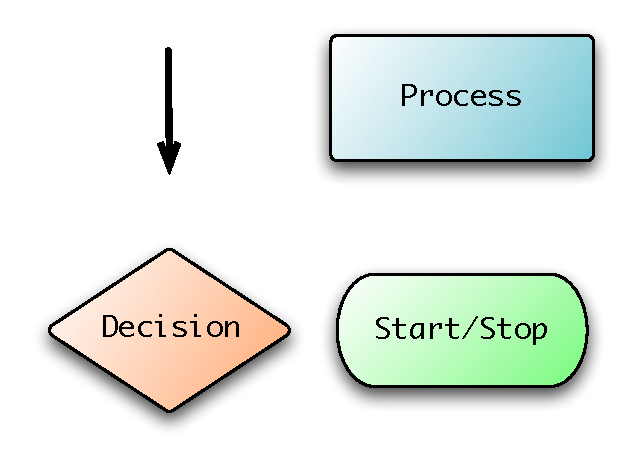
\includegraphics[width=0.5\textwidth]{./topics/control-flow/diagrams/FlowParts} 
   \caption{Flowchart Symbols}
   \label{fig:flow-symbols}
\end{figure}

% subsubsection flow_charts (end)

\clearpage
\subsubsection{Use Structured Programming Principles to guide the design of the flowchart} % (fold)
\label{ssub:structured_programming}

Flowcharts can be used to represent any sequence of actions, but not all sequences of actions will be easy to code. \fref{fig:unstructured-flow-example} is an example of a flowchart, but not one that can be coded using the structured statements covered in \cref{cha:control_flow}. \fref{fig:structured-flow-example} shows a structured version of this same algorithm. Notice that in this version there are identifiable blocks, each having a single entry and a single exit. This structure could easily be converted to code using structured statements. 

Looking at these two flowcharts, the structured flowchart looks more complicated than the unstructured version. This reflects the fact that in some cases the structured version may be more complicated, but is also an indication that this process may be better broken down into more functions and procedures. For example, the repeated loop looking for someone else to blame could be placed in its own procedure. If you find it difficult to design the control flow using structured blocks try to see if you can identify additional Functions and Procedures to help you break the code down into smaller blocks. 

\begin{figure}[htbp]
   \centering
   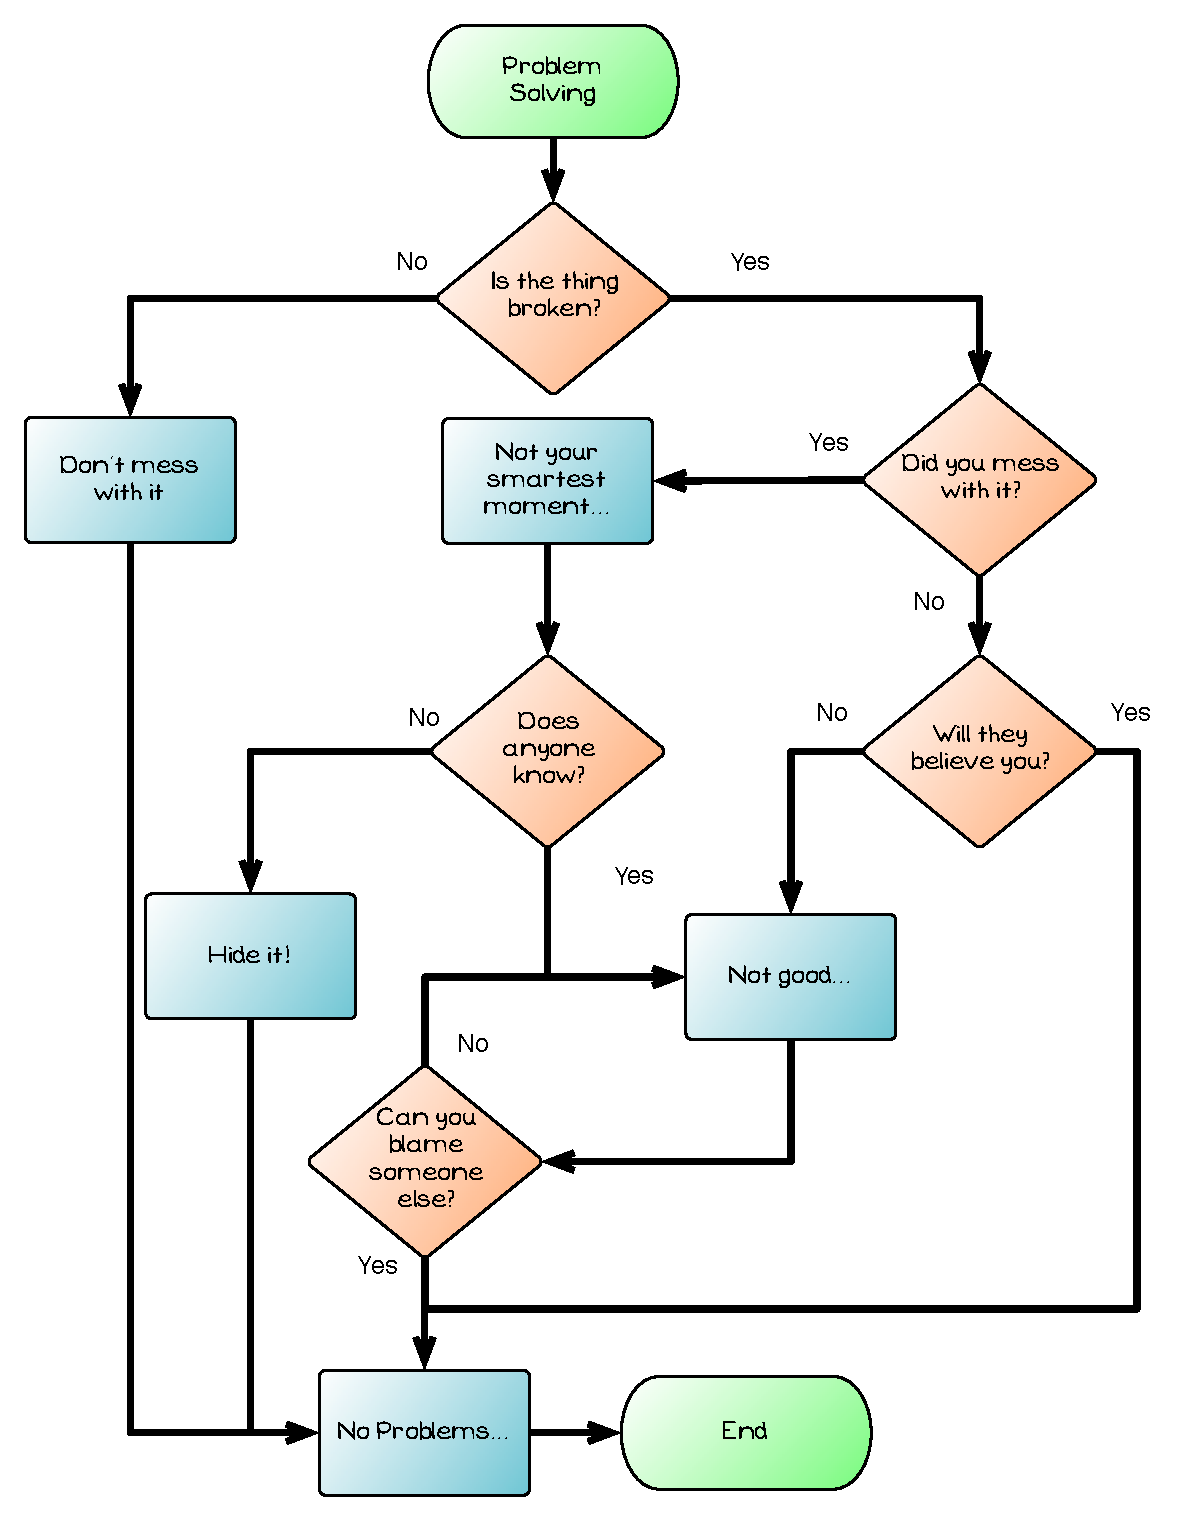
\includegraphics[width=\textwidth]{./topics/control-flow/diagrams/UnstructuredFlowSample} 
   \caption{Unstructured Flowchart}
   \label{fig:unstructured-flow-example}
\end{figure}

\begin{figure}[htbp]
   \centering
   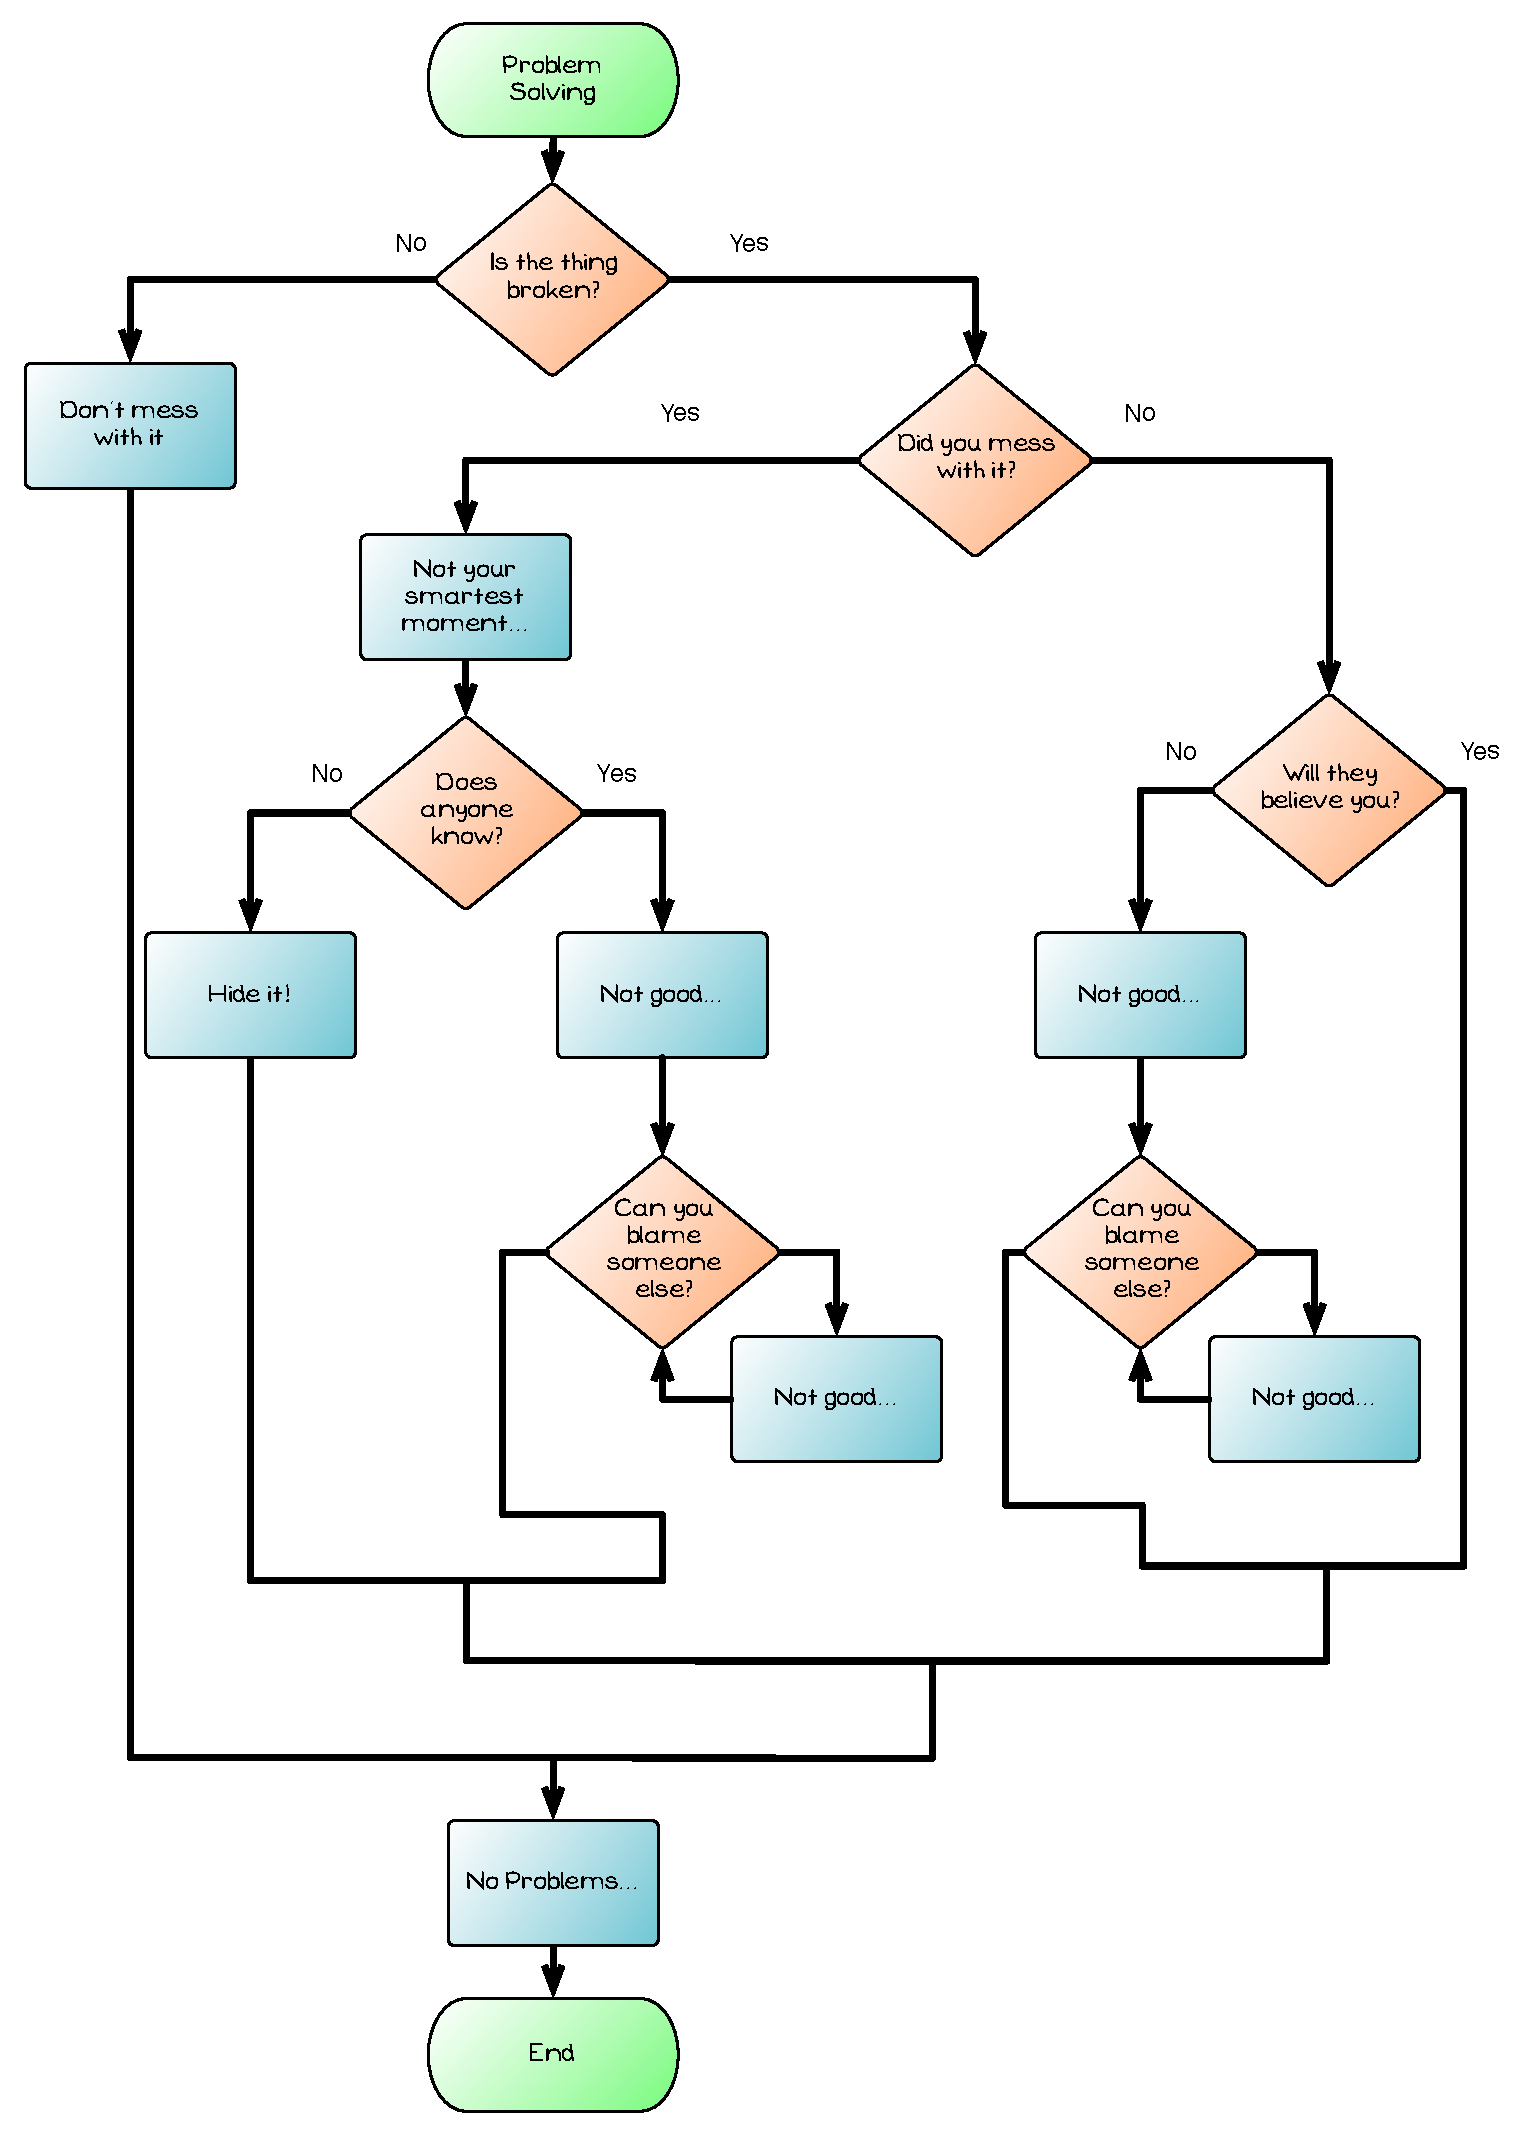
\includegraphics[width=\textwidth]{./topics/control-flow/diagrams/StructuredFlowSample} 
   \caption{Structured version of Figure \ref{fig:unstructured-flow-example}}
   \label{fig:structured-flow-example}
\end{figure}

The structured programming principles indicate that code within a Function or Procedure should be organised into \textbf{blocks}. These blocks match to the structured statements in modern programming languages: the \nameref{sub:branching} and \nameref{sub:looping} statements. Each of these blocks has a \textbf{single entry point} and a \textbf{single exit point}, allowing them to combined together.

The addition of \nameref{sub:jump} statements to the language allows the blocks to have \textbf{multiple exit points}; one at the end of the block's code, the other at a \nameref{sub:break}, \nameref{sub:exit}, or \nameref{sub:return_statement}. These statements give you extra flexibility, but still work within the structured programming principles.

\mynote{
Prior to the Structured Programming, programs had two control flow mechanisms: \texttt{if} and \nameref{sub:goto}. Control flow was not easy to picture or understand. Programs written in this way are now know as \textbf{spaghetti code}, as understanding this code is much like trying to untangle a bowl of spaghetti, though not nearly as tasty.
}
% subsubsection structured_programming (end)

\clearpage
\subsubsection{The Structured Programming blocks used to build the logic} % (fold)
\label{ssub:structured_programming_blocks}

In Structured Programming there are three kinds of blocks:
\begin{itemize}
  \item \textbf{Sequence}: one instruction follows the next in a sequence.
  \item \textbf{Selection}: the ability to branch the sequence.
  \item \textbf{Repetition}: repeat a block a number of times.
\end{itemize}

The flowchart snippets in the section on \nameref{sub:branching} and \nameref{sub:looping} showed how the flows work for \emph{selection} and \emph{repetition}. \fref{fig:selection-flow} shows the three alternatives for selection blocks, \fref{fig:repetition-flow} shows the two alternatives for repetition blocks, and \fref{fig:sequence-flow} shows the standard sequence flow. The design of any program's logic is a task in combining these blocks together to perform the desired effect. 

\begin{figure}[h]
   \centering
   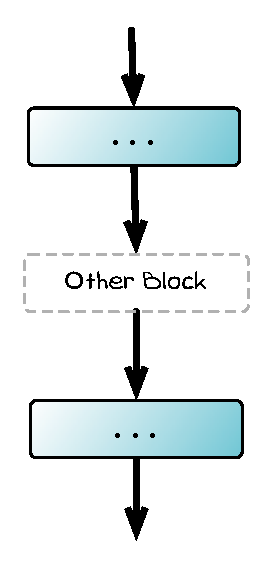
\includegraphics[width=0.15\textwidth]{./topics/control-flow/diagrams/SequenceFlow} 
   \caption{Flows for Sequence Blocks}
   \label{fig:sequence-flow}
\end{figure}

\begin{figure}[h]
   \centering
   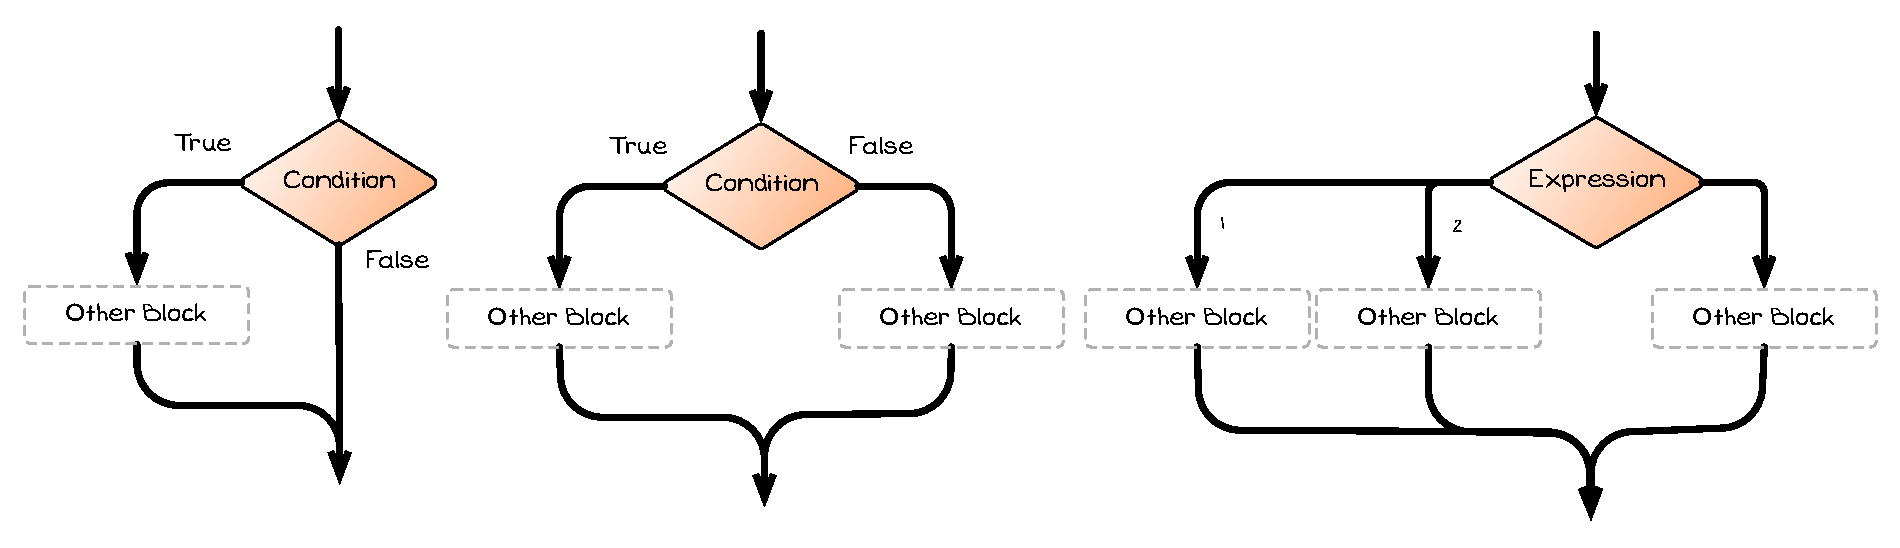
\includegraphics[width=0.9\textwidth]{./topics/control-flow/diagrams/SelectionFlow} 
   \caption{Flows for Selection Blocks}
   \label{fig:selection-flow}
\end{figure}

\begin{figure}[h]
   \centering
   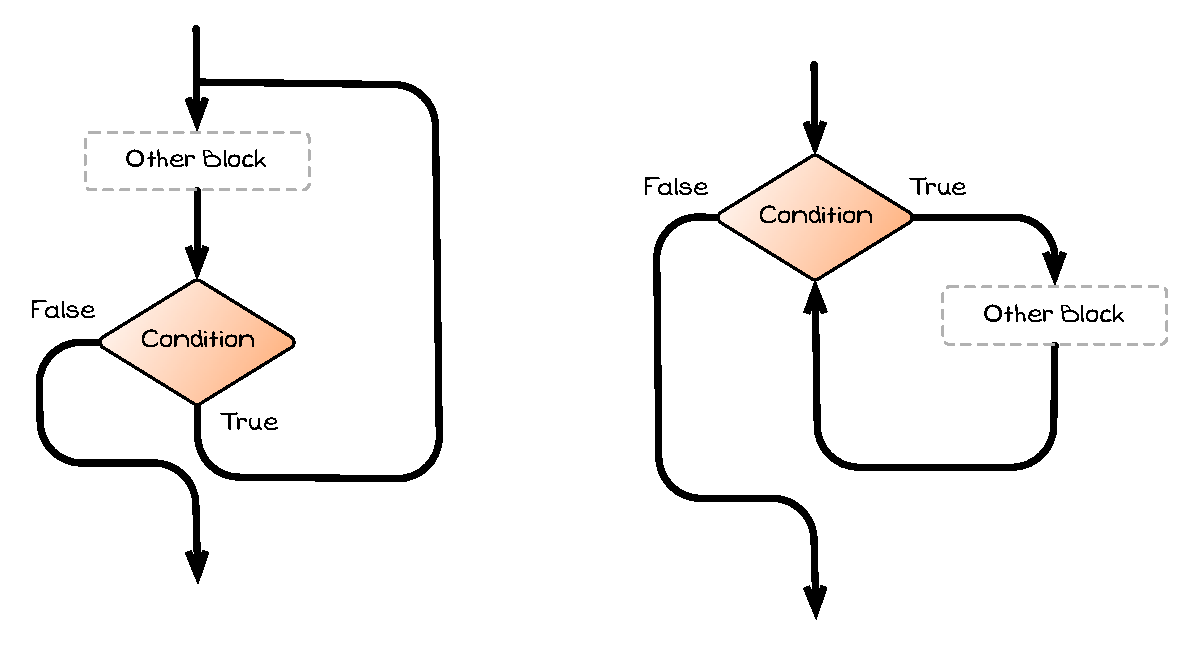
\includegraphics[width=0.55\textwidth]{./topics/control-flow/diagrams/RepetitionFlow} 
   \caption{Flows for Repetition Blocks}
   \label{fig:repetition-flow}
\end{figure}

% subsubsection structured_programming_blocks (end)

\subsubsection{Combining blocks for the Perform Guess} % (fold)
\label{ssub:combining_blocks_for_the_guessing_game}

With the basic theory at hand, we can now start to design the control flow for the Guess that Number program. This process will involve, once again, the idea of \textbf{abstraction}. When designing the flow for a program you first need to be able to perform the process yourself, even if its just on paper, and then work out the steps that you undertook so that you can code these within the program.

For the Guess that Number program we can start by designing the control flow within the \texttt{Perform Guess} function. The specification of this is shown in \tref{tbl:perform guess}. Think about the steps that need to be performed to achieve this. If you had been asked to do this what would you need to do?

\begin{table}[h]
  \centering
  \begin{tabular}{|c|p{9cm}|}
    \hline
    \multicolumn{2}{|c|}{\textbf{Function}} \\
    \hline
    \multicolumn{2}{|c|}{} \\
    \multicolumn{2}{|c|}{\texttt{Perform Guess}} \\
    \multicolumn{2}{|c|}{} \\
    \hline
    \multicolumn{2}{|c|}{\textbf{Returns}} \\
    \hline
    \texttt{Boolean} & True when the user has guessed the number, False otherwise. \\
    \hline
    \textbf{Parameter} & \textbf{Description} \\
    \hline
    \texttt{Guess Number} & The number of the current guess, used in the prompt asking for the user to enter their guess. \\
    & \\
    \texttt{Target}   & The number the user is aiming to guess. \\
    \hline
    \multicolumn{2}{|c|}{} \\
    \multicolumn{2}{|p{12cm}|}{Perform Guess is responsible for coordinating the actions needed to perform a single guess within a game of \emph{Guess that Number}. The user's \texttt{guess} is read, and the value checked against the \texttt{target} value. A message is then output telling the user if the target value is less than, larger than, or equal to their guess. This function returns True when the user's guess is equal to the target.} \\
    \multicolumn{2}{|c|}{} \\
    \hline
  \end{tabular}
  \caption{Specification for the \texttt{Perform Guess} Function.}
  \label{tbl:perform guess}
\end{table}

The first task the Function needs to perform is to get the guess from the user. This can be performed in a \textbf{sequence}: display a prompt, read the value from the user. This first sequence is shown in \fref{fig:perform-guess-seq-1}.

\begin{figure}[h]
   \centering
   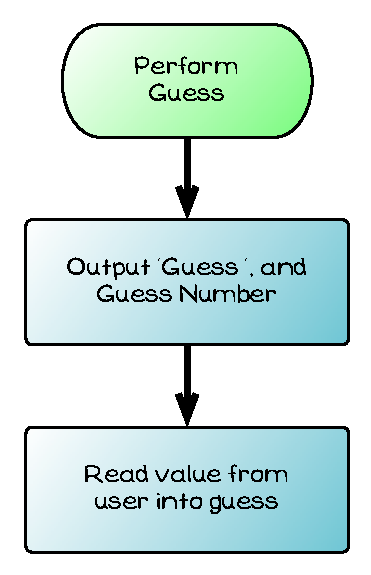
\includegraphics[width=0.25\textwidth]{./topics/control-flow/diagrams/PerformGuess1} 
   \caption{Initial Sequence in \texttt{Perform Guess}}
   \label{fig:perform-guess-seq-1}
\end{figure}

\clearpage
The next step in this sequence is to give the user feedback based upon their guess and the target number. This code requires a the ability to \emph{select} a given branch. The computer needs to output different messages based upon the users guess. This can be achieved with a \textbf{selection} block. Looking back at \fref{fig:selection-flow} there are three possible alternatives for implementing this selection. The \texttt{if} with no \texttt{else} is not a valid option as there are three paths we need to take. The \texttt{case} block is also not valid as we are not matching a value, but comparing values to each other. The last option is the \texttt{if-else} block, but this only has two branches. It is not going to be possible to code all three options within one block, but it can be achieved using two \texttt{if-else} blocks.

The first \texttt{if-else} block will check if the \texttt{target} is greater than the user's \texttt{guess}. If this is true then the computer can take the first branch and output the message `The number is larger than ' and the value from the user's guess. The flow chart for this part is shown in \fref{fig:perform-guess-seq-2}. This block is the third task in the sequence, this if block has a single entry, causes a branch in the flow, and will have a single exit.

\begin{figure}[h]
   \centering
   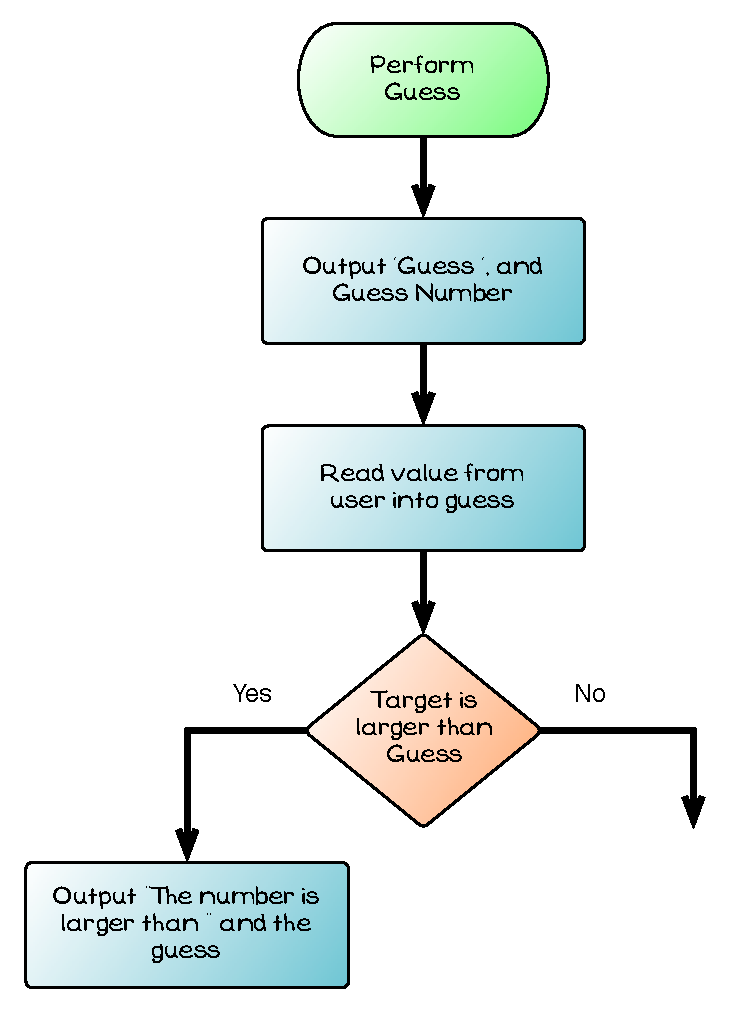
\includegraphics[width=0.6\textwidth]{./topics/control-flow/diagrams/PerformGuess2} 
   \caption{First branch in \texttt{Perform Guess}}
   \label{fig:perform-guess-seq-2}
\end{figure}

\mynote{
\begin{itemize}
  \item The conditions within the \nameref{sub:if_statement} are Boolean Expressions.
  \item This condition is checking if \texttt{target > guess}.
  \item There are now two paths through this code, one when \texttt{target} is \texttt{> guess}, and another when it is not.
\end{itemize}
}

\clearpage

Following the false path from the first decision, and we have a new location into which to insert a block. At this point we know the target is \emph{not} larger than the user's guess. At this point you can include another \texttt{if-else} block to check if the target is \textbf{less than} the user's guess. This is shown in \fref{fig:perform-guess-seq-3}.

\begin{figure}[htbp]
   \centering
   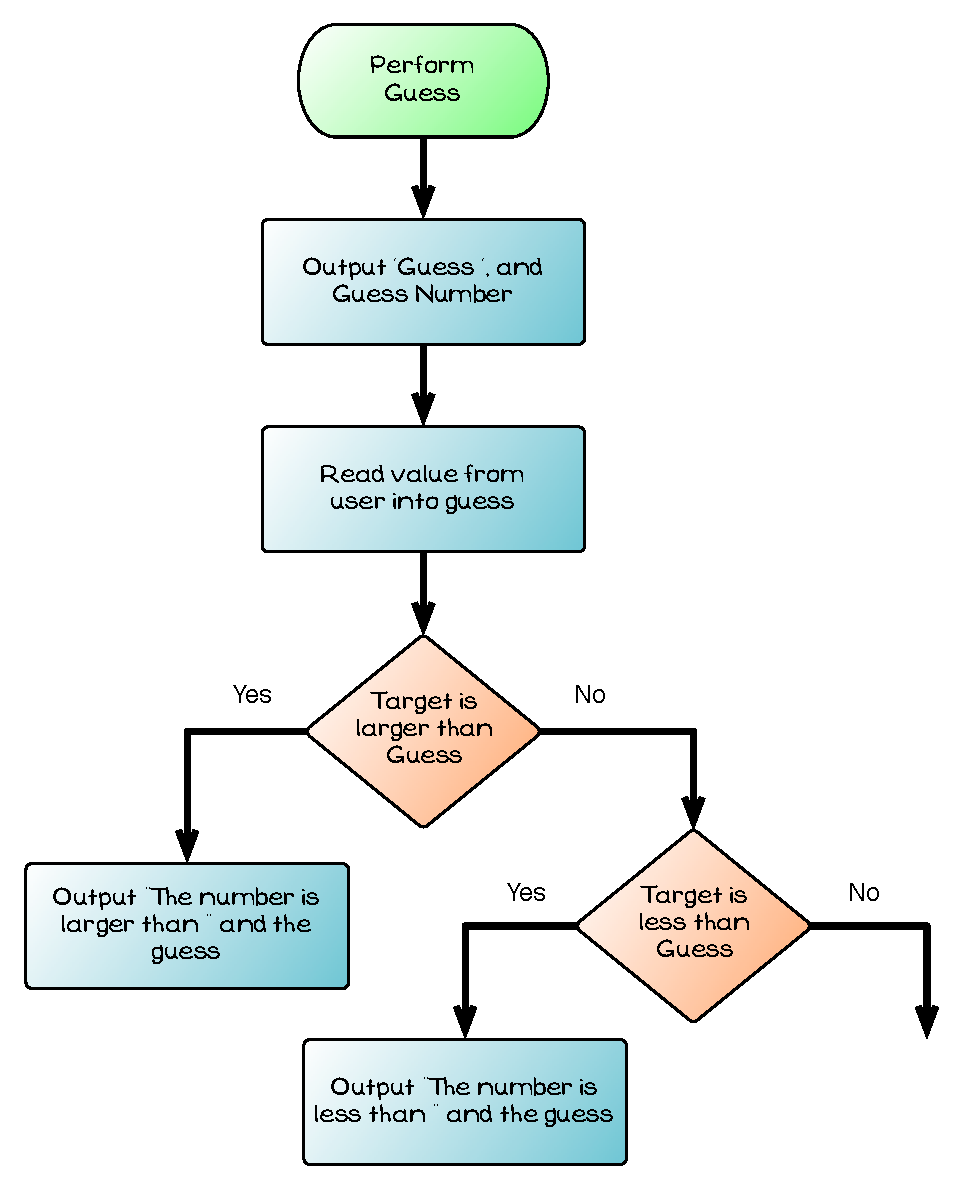
\includegraphics[width=0.7\textwidth]{./topics/control-flow/diagrams/PerformGuess3} 
   \caption{Second branch tests if the Target is less than the guess}
   \label{fig:perform-guess-seq-3}
\end{figure}

\mynote{
\begin{itemize}
  \item The newly added block is another \nameref{sub:if_statement}.
  \item This is nested within the \texttt{else} branch of the first If Statement.
  \item This code checks \emph{if} \texttt{target < guess}.
  \item There are now three paths through this code.
\end{itemize}
}

\clearpage
Taking the false path again, and now we have a location at which the target value \emph{must be} equal to the user's guess. The first condition checked if the \texttt{target} was larger than the \texttt{guess}, which it was not. The second condition checked if the \texttt{target} was less than the \texttt{guess}, which it was not. So the only way this can be the case if is the \texttt{target} and the \texttt{guess} are equal. This path can then be used to output the `Well done\ldots' message. This is shown in \fref{fig:perform-guess-seq-4}. 

\begin{figure}[htbp]
   \centering
   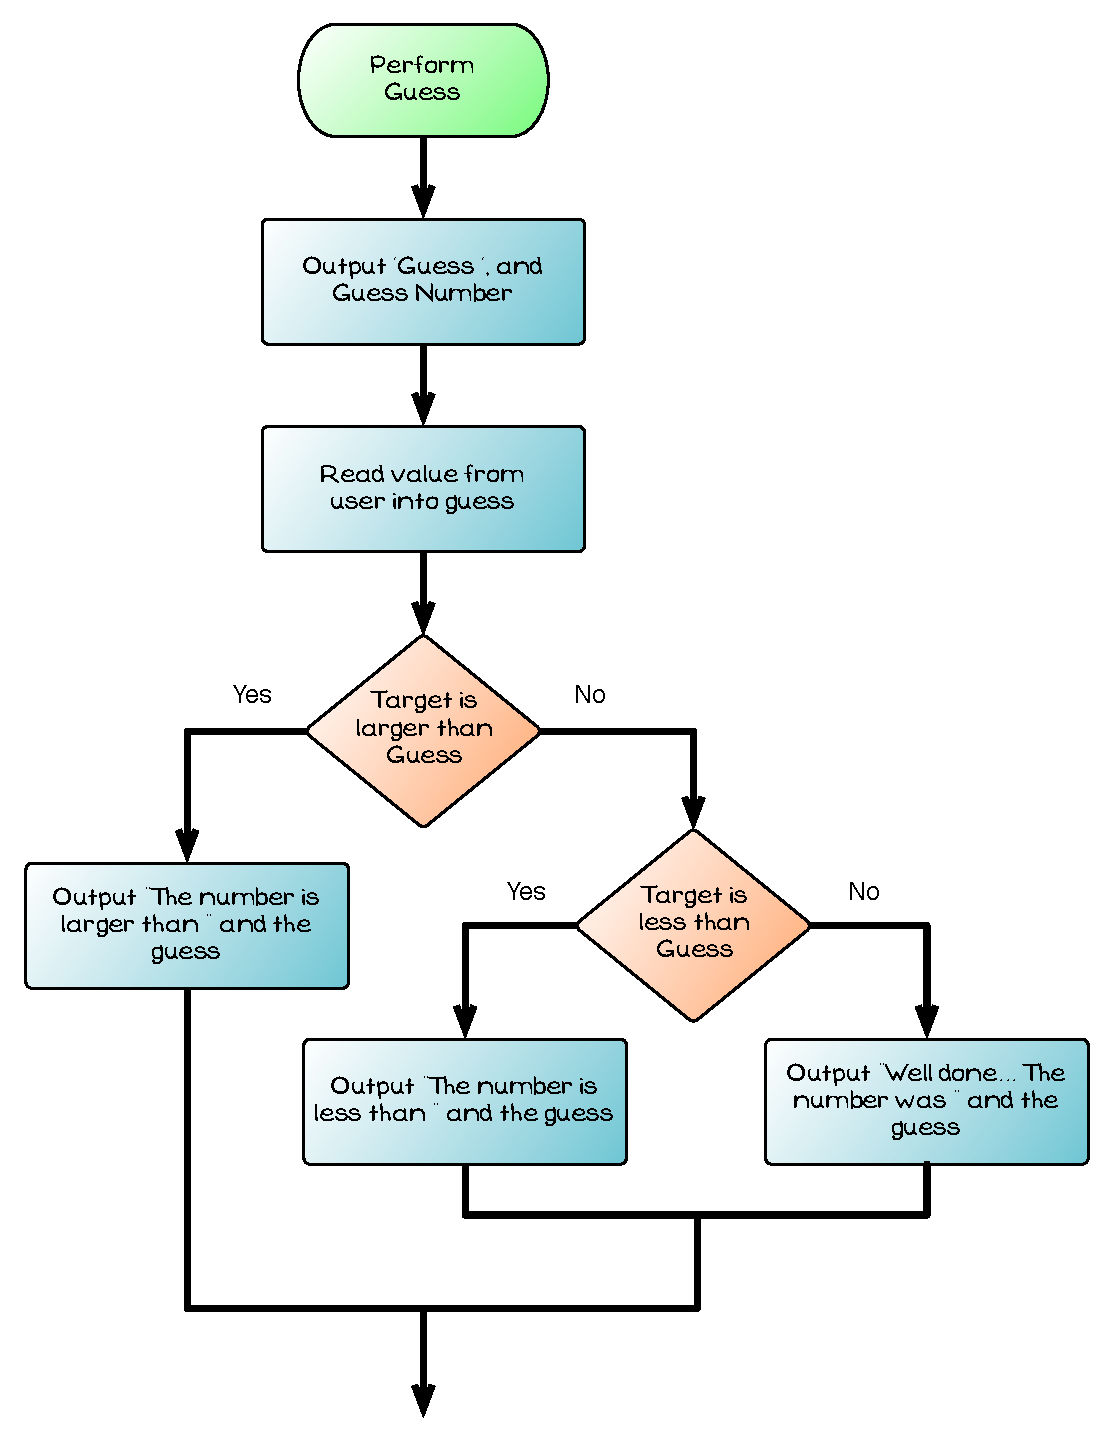
\includegraphics[width=0.8\textwidth]{./topics/control-flow/diagrams/PerformGuess4} 
   \caption{The `Well done\ldots' message can be output on the third path}
   \label{fig:perform-guess-seq-4}
\end{figure}

\mynote{
\begin{itemize}
  \item The newly added block is a sequence, outputting the `Well done\ldots' message.
  \item On this third path the \texttt{target} and \texttt{guess} must be equal.
  \item Notice the single exit out of the second branch, when then flows to the single exit out of the first branch.
\end{itemize}
}

\clearpage
The last action in the code is to return a Boolean result indicating if the user's guess is equal to the target number.

\begin{figure}[htbp]
   \centering
   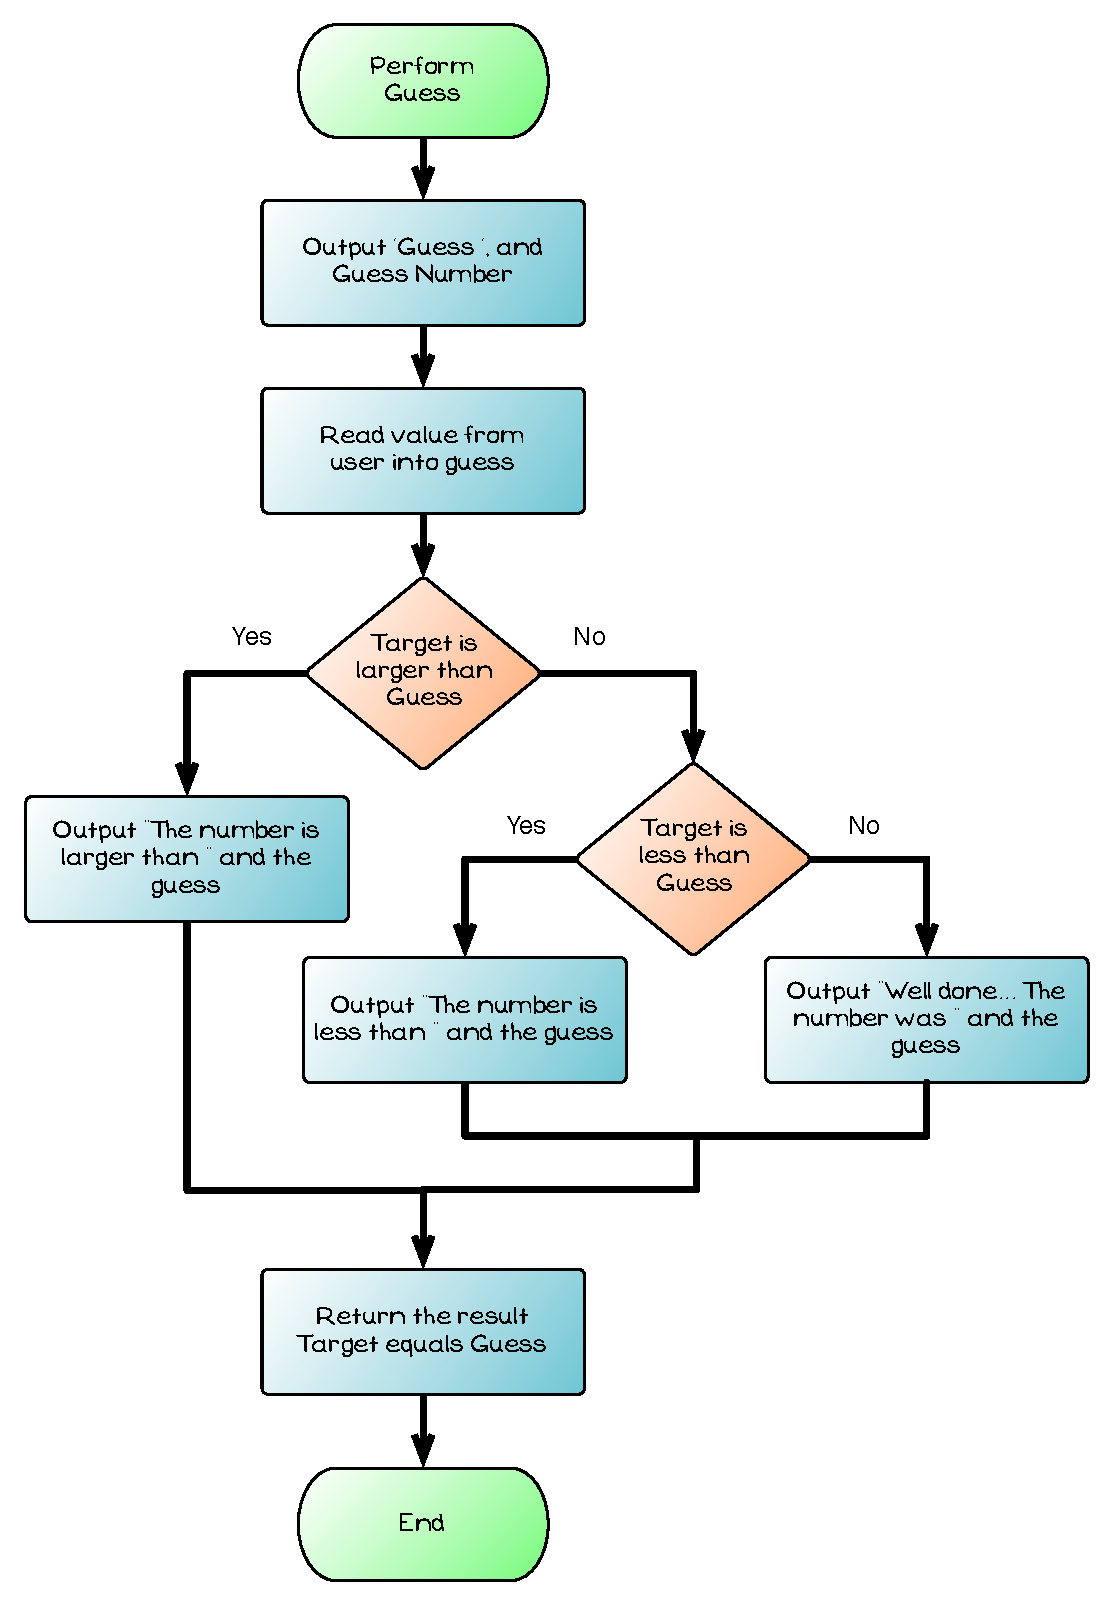
\includegraphics[width=0.74\textwidth]{./topics/control-flow/diagrams/PerformGuess5} 
   \caption{A Boolean result is returned from the Function}
   \label{fig:perform-guess-seq-5}
\end{figure}

\mynote{
\begin{itemize}
  \item The newly added block is a single action, defining the result to be returned.
  \item This action returns the result True when the \texttt{target} and the \texttt{guess} are equal.
\end{itemize}
}

\clearpage

\fref{fig:perform-guess-seq-7} shows the flowchart with annotations highlighting the different blocks within the code. The function starts off with a \textbf{sequence} that contains all of the code in the Function. Within this there is the \textbf{selection}, that internally contains another \textbf{selection}.

\begin{figure}[htbp]
   \centering
   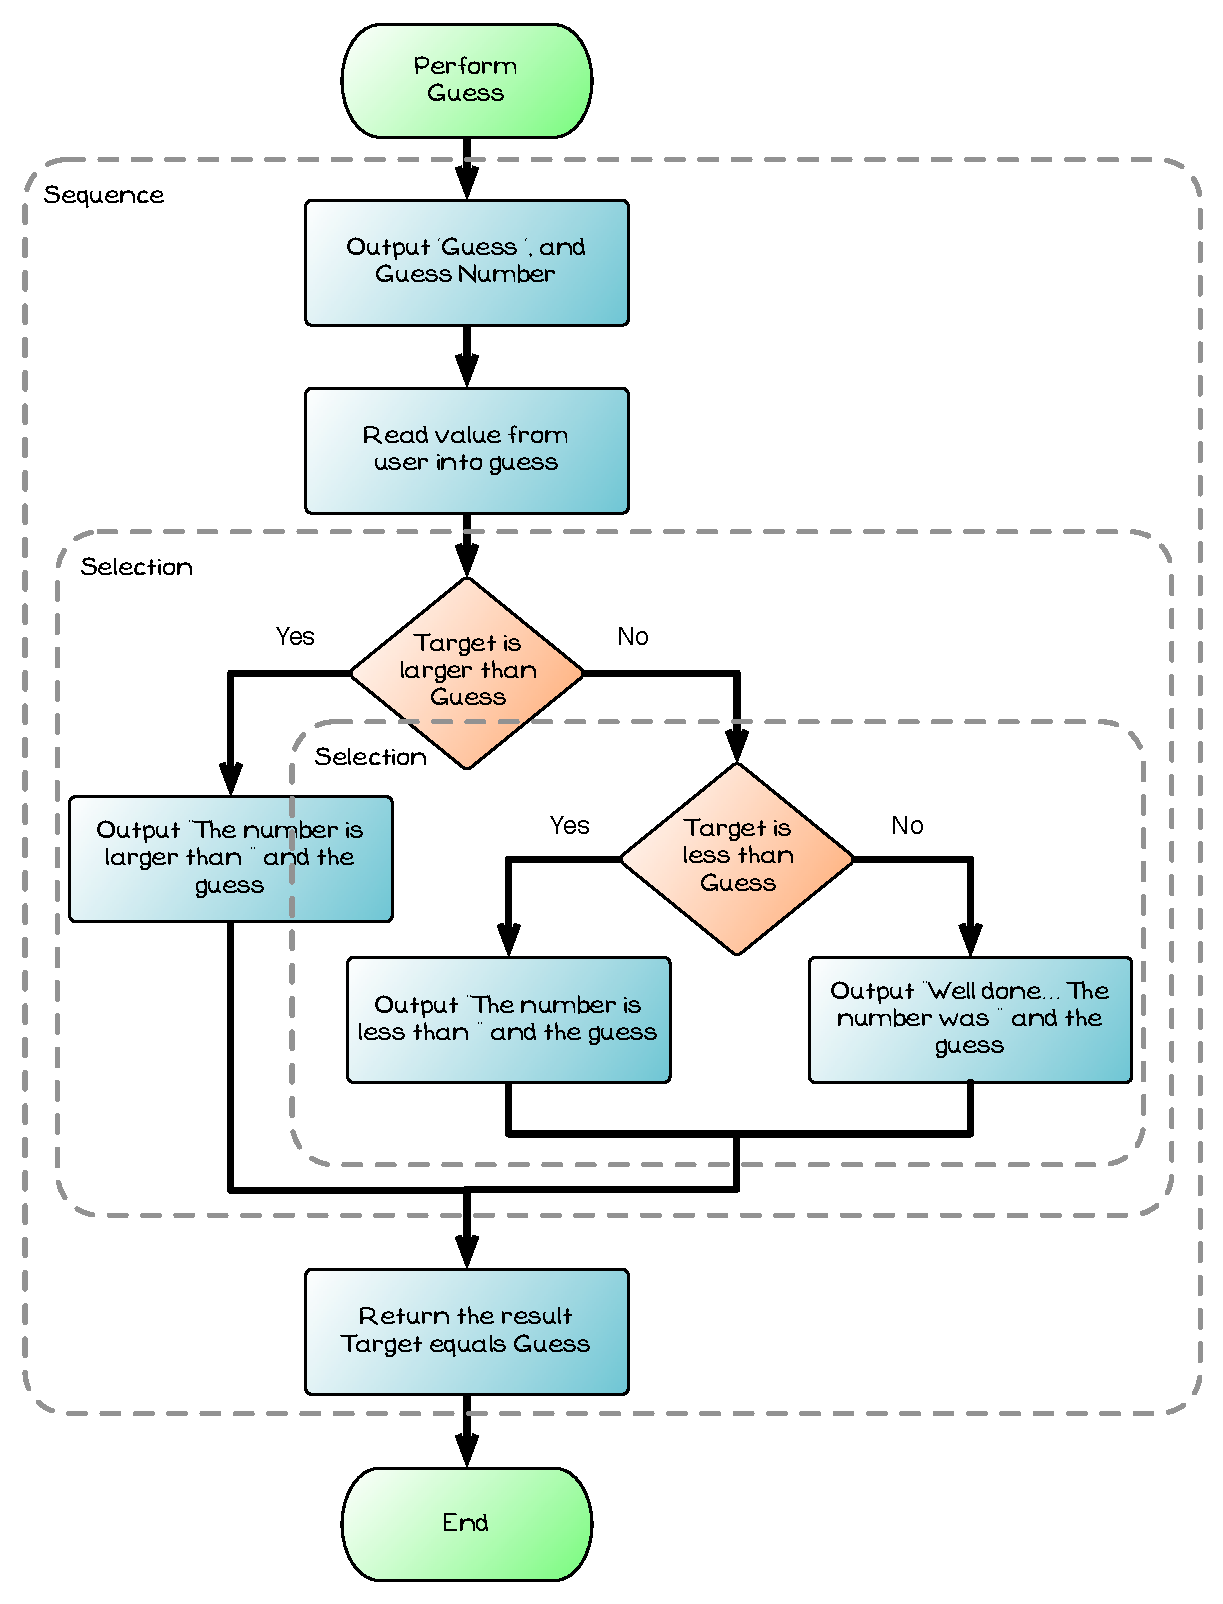
\includegraphics[width=0.85\textwidth]{./topics/control-flow/diagrams/PerformGuess7} 
   \caption{Blocks in the \texttt{Perform Guess} code}
   \label{fig:perform-guess-seq-7}
\end{figure}

\mynote{
\begin{itemize}
  \item Notice that each block has a single path going into it, and a single path coming out.
\end{itemize}
}

% subsubsection combining_blocks_for_the_guessing_game (end)

\clearpage
\subsubsection{Setting the result using an Expression} % (fold)
\label{ssub:setting_the_result_using_an_expression}

\fref{fig:perform-guess-seq-6} shows the \emph{trick} that is being performed at the end of \texttt{Perform Guess}'s code. \texttt{Perform Guess} needs to return a result indicating if the user has guessed the number of not. This will be a Boolean value, with True indicating they guessed the number. Initially it may seem that you need a \textbf{selection} block to enable this, as shown on the right of \fref{fig:perform-guess-seq-6}. 

\begin{figure}[htbp]
   \centering
   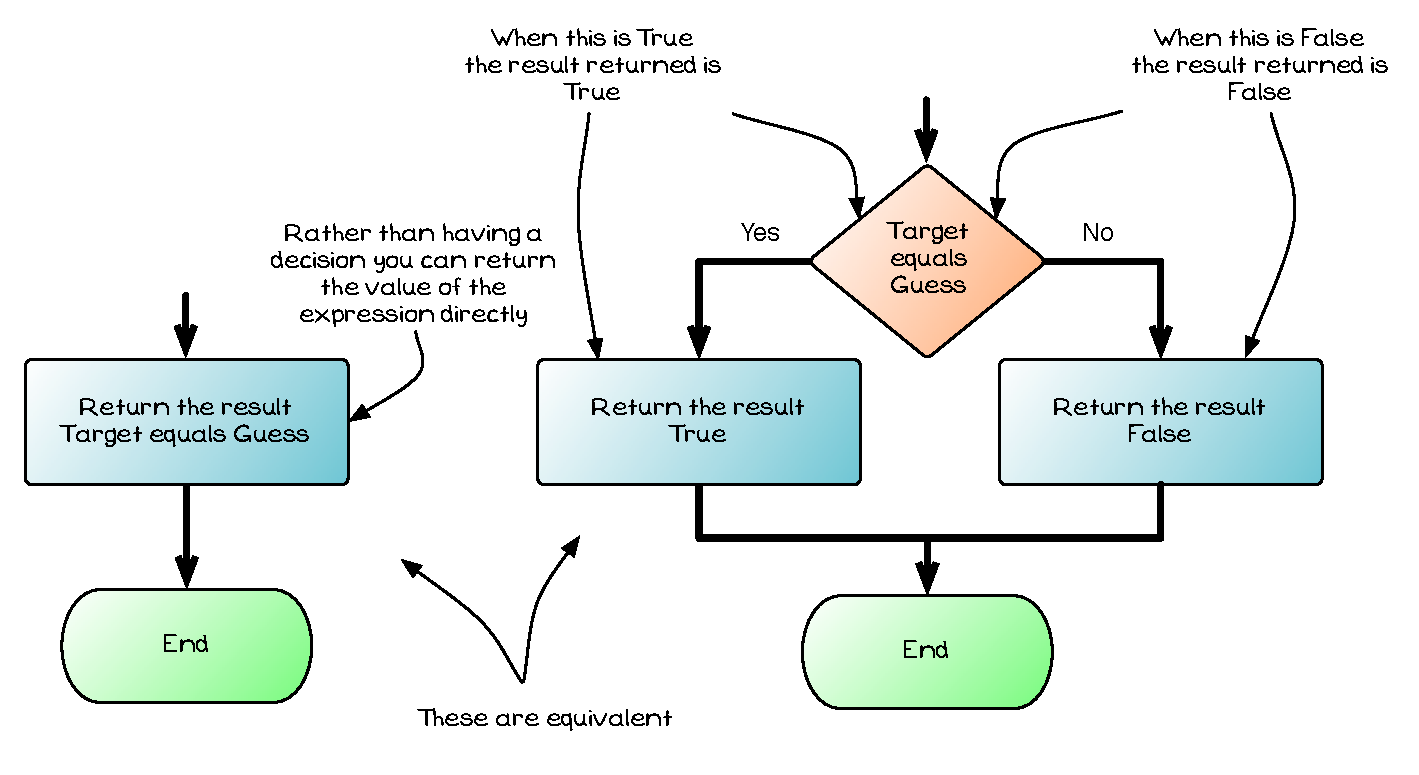
\includegraphics[width=\textwidth]{./topics/control-flow/diagrams/PerformGuess6} 
   \caption{Calculating \texttt{Perform Guess}'s result}
   \label{fig:perform-guess-seq-6}
\end{figure}

\mynote{
\begin{itemize}
  \item In \emph{most} cases it is better to have less code if possible, as long as this does not obscure the purpose of the code.
  \item This is an example of replacing \emph{actions} with \emph{data}. The more \emph{intelligence} you can build into the data in your programs the more flexible they will be.
\end{itemize}
}

\csection{This is achieved in C using \csnipet{return target == guess;}}

\passection{This is achieved in Pascal using \passnipet{result := target = guess;}}


% subsubsection setting_the_result_using_an_experssion (end)

\clearpage
\subsubsection{The Pseudocode for \texttt{Perform Guess}} % (fold)
\label{ssub:the_pseudocode_for_perform_guess}

Listing \ref{plst:perform_guess} contains the Pseudocode for the \texttt{Perform Guess} logic from the flowchart in \fref{fig:perform-guess-seq-5}. Notice how the indentation in this mirrors the block structures in the flowchart. It is good practice to indent your code in this way as it helps you, and any person who reads your code, to see the structure of the logic. You will be able to avoid many errors by making sure that you always indent your code so that it highlights the code's structure.

\pseudocode{plst:perform_guess}{Pseudocode for \texttt{Perform Guess}}{topics/control-flow/application/PerformGuess.txt}

\mynote{
\begin{itemize}
  \item Code indentation makes it easier to read, and helps locate many common issues.
  \item Tab you code in within a \textbf{structured statement}.
  \begin{itemize}
    \item Indent the code in the branches of an \nameref{sub:if_statement} and \nameref{sub:case_statement}.
    \item Indent the code within the body of the \textbf{While Loop} and the \textbf{Do While} or \textbf{Repeat Until} loops. 
  \end{itemize}
  \item Make this a habit. When you code a \nameref{sub:branching} or \nameref{sub:looping} statement automatically indent the next line of code.
  \item Always keep you code neat, make it look good.
  \item The C code for \texttt{Perform Guess} is shown in Listing \ref{clst:perform_guess}.
  \item The Pascal code for \texttt{Perform Guess} is shown in Listing \ref{paslst:perform_guess}.
  \item Notice how the two code samples are laid out in a similar way. The indentation makes it easy to identify which statements are associated with each of the branches through the Function. 
\end{itemize}
}

\clearpage

\csection{\ccode{clst:perform_guess}{C code for \texttt{Perform Guess}}{topics/control-flow/application/perform-guess.c}}

\passection{\pascode{paslst:perform_guess}{Pascal code for \texttt{Perform Guess}}{topics/control-flow/application/PerformGuess.pas}}


% subsubsection the_pseudocode_for_ (end)


% subsection designing_control_flow_for_guess_that_number (end)

\clearpage
\subsection{Designing Control Flow for Play Game} % (fold)
\label{sub:designing_control_flow_for_play_game}

The \texttt{Play Game} Procedure is another artefact that will require some some thought to design its logic. \tref{tbl:play game} contains the specification for this Procedure. It will be responsible for coordinating the actions of the game, while \texttt{Perform Guess} coordinates the actions for a \emph{single} guess.

\begin{table}[h]
  \centering
  \begin{tabular}{|c|p{9cm}|}
    \hline
    \multicolumn{2}{|c|}{\textbf{Procedure}} \\
    \hline
    \multicolumn{2}{|c|}{} \\
    \multicolumn{2}{|c|}{\texttt{Play Game}} \\
    \multicolumn{2}{|c|}{} \\
    \hline
    \multicolumn{2}{|c|}{} \\
    \multicolumn{2}{|p{12cm}|}{Play Game is responsible for coordinating the actions involved in playing a single game of \emph{Guess that Number}. Initially the computer will generate a random target value, and output starting text. Then it will repeatedly ask the user to guess the number, until either the user has guessed the value or they have run out of guesses. If the user does run out of guesses then the computer ends the game, and tell the user the target value.} \\
    \multicolumn{2}{|c|}{} \\
    \hline
  \end{tabular}
  \caption{Specification for the \texttt{Play Game} Procedure.}
  \label{tbl:play game}
\end{table}

The implementation of this Procedure will require us to store some data. The following \nameref{sub:local_variable}s will be needed to store data within this Procedure:
\begin{itemize}
  \item \texttt{\textbf{My Number}}: This will store the computer's randomly chosen number.
  \item \texttt{\textbf{Guess Number}}: This will store the current guess the user is at, allowing the computer to stop looping when the number of guesses is exceeds 7.
  \item \texttt{\textbf{Got It}}: A Boolean value to indicate if the user did guess the number, allowing the computer to stop looping when the user guesses the number.
\end{itemize}

The flowchart for this is shown in \fref{fig:play-game}, and again in \fref{fig:play-game-diag1} with its blocks highlighted. This code uses a \textbf{repetition} to ask the user to perform up to 7 guesses. The condition on this loop occurs \emph{after} the loop body as the user must have at least one guess. 

There is also a \textbf{selection} after the loop to output the answer if the user ran out of guesses. This is only done when the user has not guessed it themselves. This does not need to perform any other actions when the user did guess the number, so the False branch has no additional actions. In code this would be implemented with an \nameref{sub:if_statement} without an \textbf{else} branch.

\mynote{
\begin{itemize}
  \item A loop may have its condition before or after its instructions.
  \item If the condition is after the loop, as it is with \texttt{Play Game}, then this gives a loop that runs at least once.
  \item The else branch on the If Statement is optional. If you have no processing for this branch you leave the \texttt{else} off in the code.
  \item The condition of the If Statement in \texttt{Play Game} check if the \texttt{Got It} is False using the \texttt{not} logical operator.
\end{itemize}
}

\begin{figure}[htbp]
   \centering
   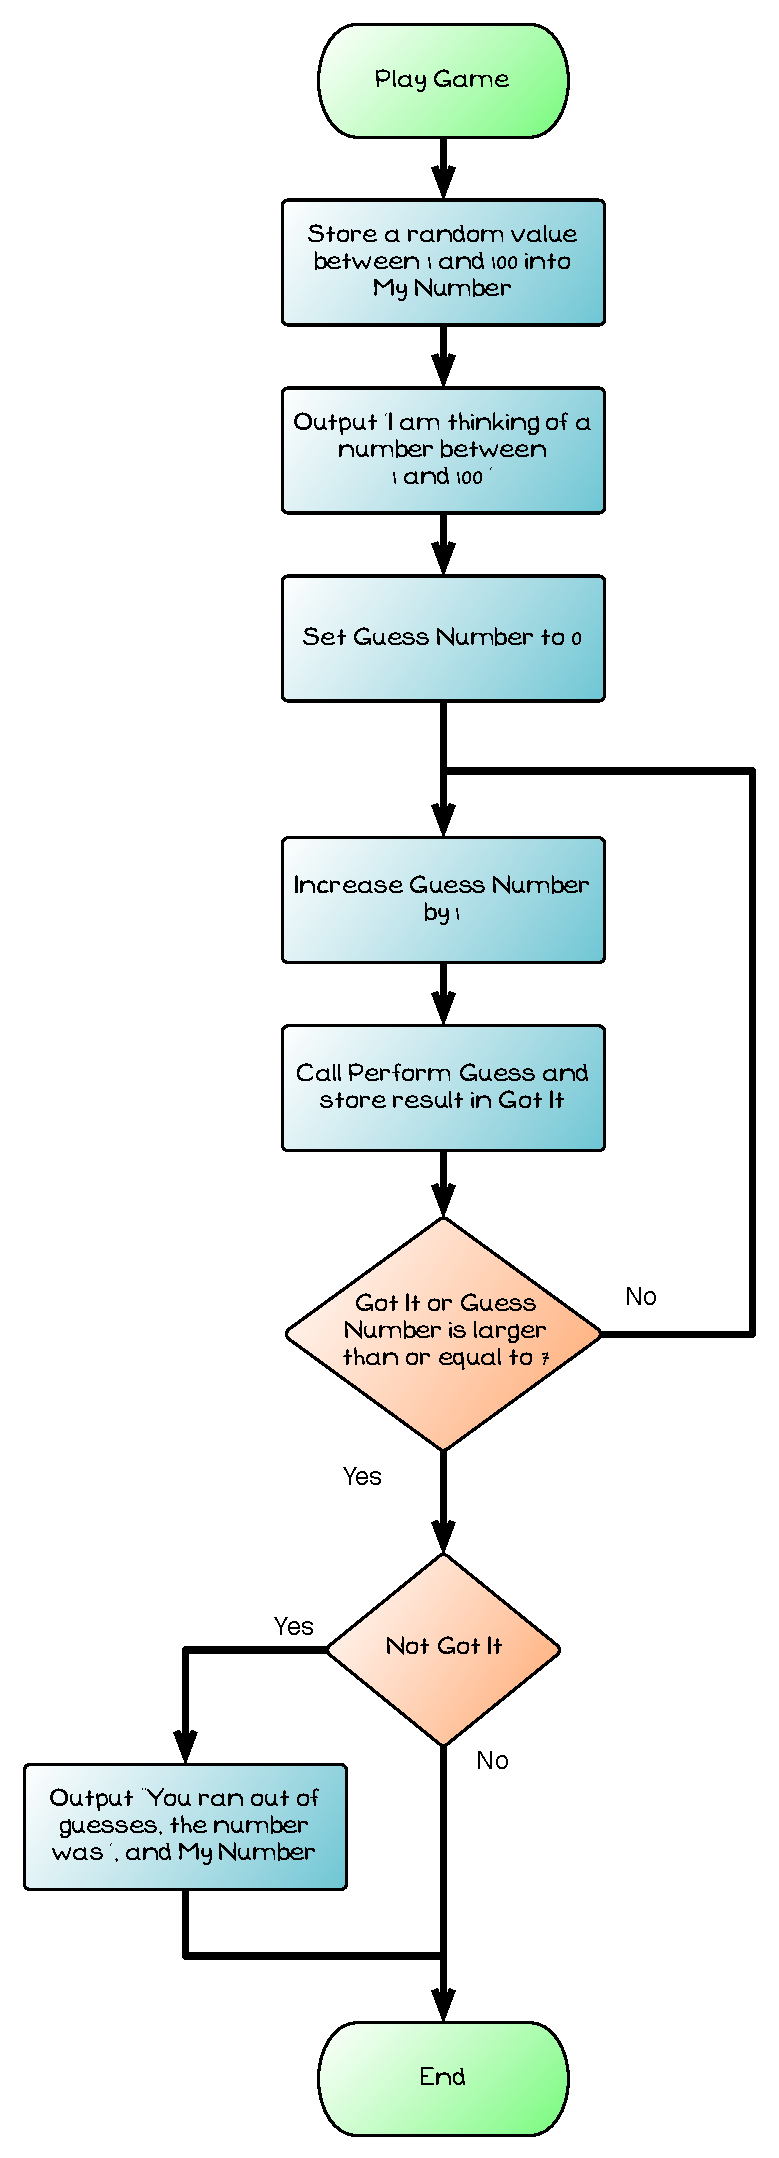
\includegraphics[width=0.52\textwidth]{./topics/control-flow/diagrams/PlayGame} 
   \caption{Logic for the \texttt{Play Game} Procedure}
   \label{fig:play-game}
\end{figure}

\begin{figure}[htbp]
   \centering
   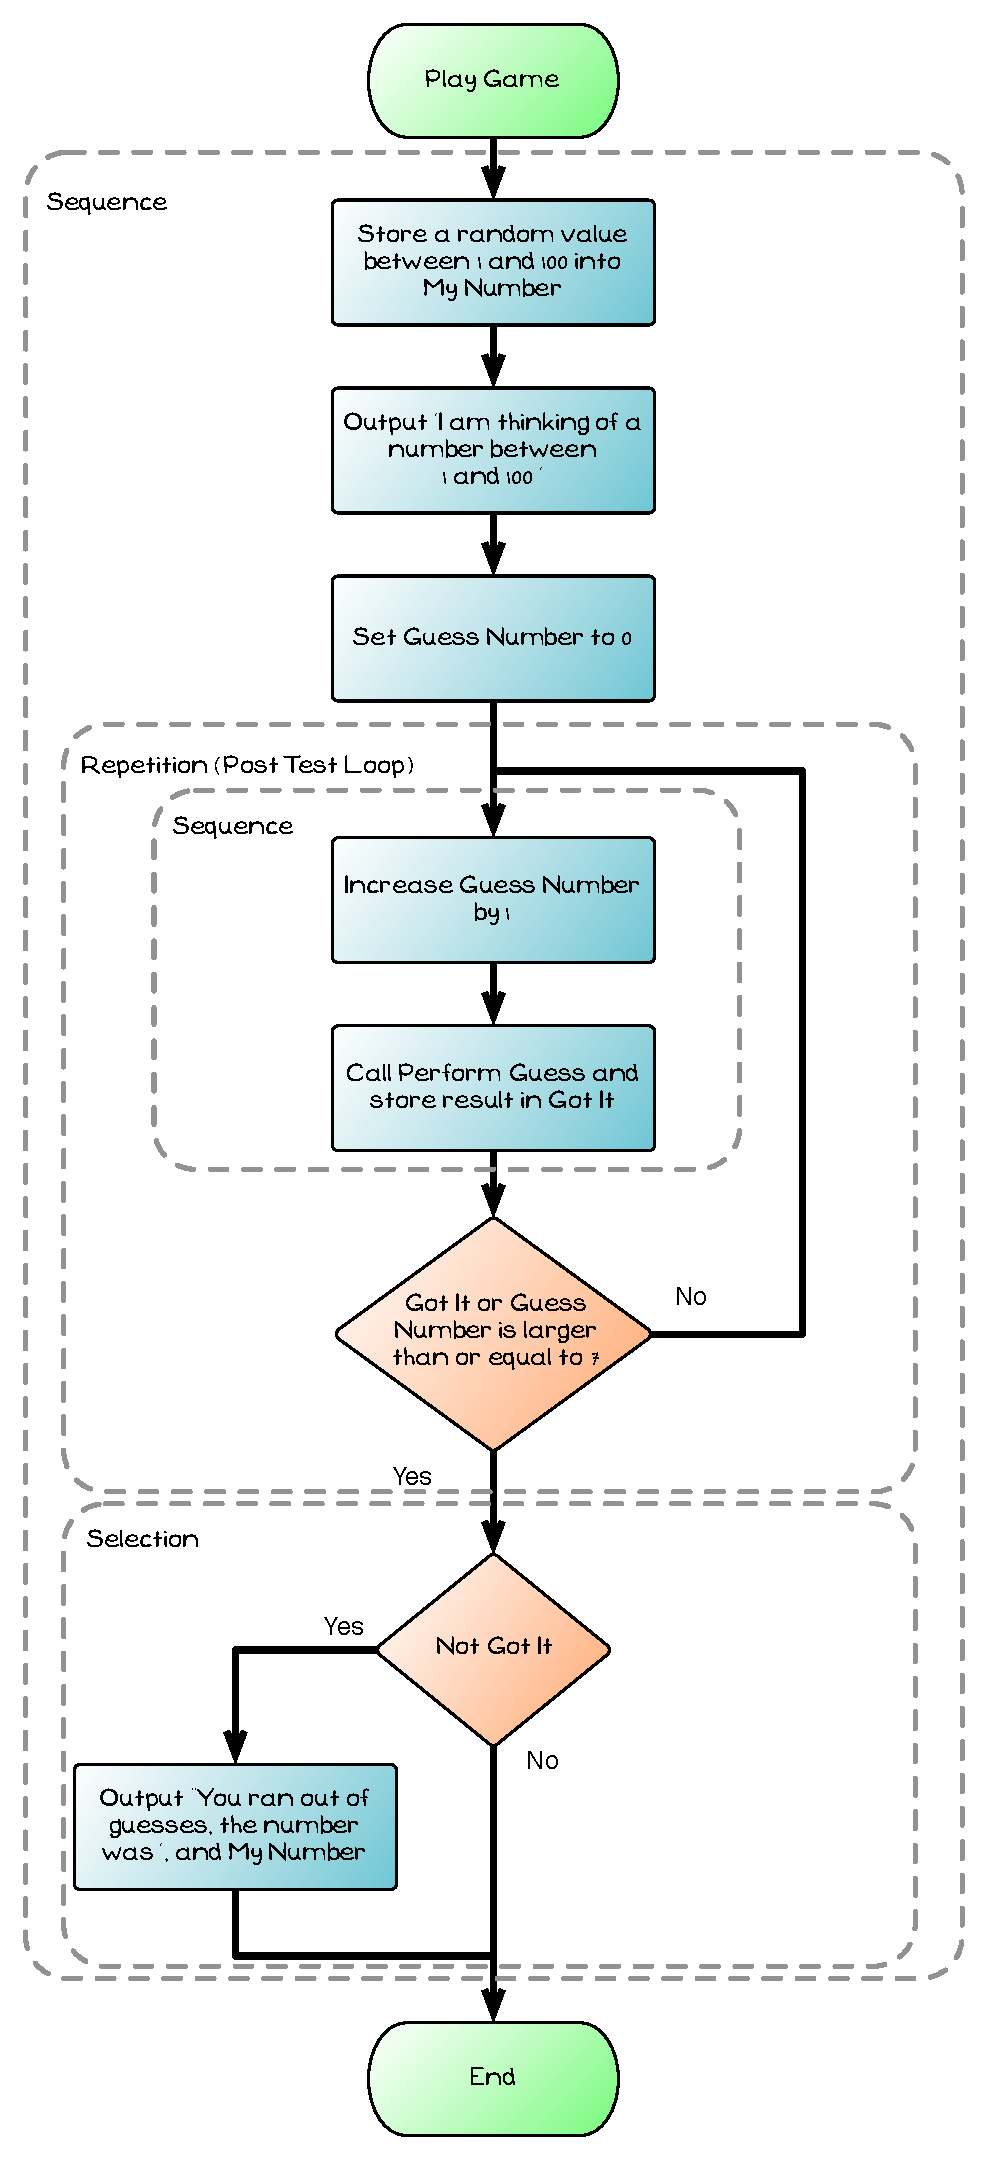
\includegraphics[width=0.65\textwidth]{./topics/control-flow/diagrams/PlayGame1} 
   \caption{Blocks in the \texttt{Play Game} code}
   \label{fig:play-game-diag1}
\end{figure}

\clearpage

\lref{plst:play_game} contains the Pseudocode for the \texttt{Play Game} Procedure. This uses Constants for \texttt{MAX\_NUMBER} and a \texttt{MAX\_GUESSES}, this will make it easier to change the range of the numbers and the associated number of guesses.

The flowchart for \texttt{Play Game} includes a \nameref{sub:post_test_loop}, which can be coded as either a \texttt{do...while} or a \texttt{repeat...until} loop. This two variations are shown in step 7 of \lref{plst:play_game}, with the while version appearing as a comment on the following line. Both of these versions have the same result, but do require different conditions. The two implementations of this are shown in \lref{clst:play_game} and \lref{paslst:play_game}. It is important to understand that the basic ideas of a \textbf{post-test loop} is the same regardless of whether it is coded using \texttt{do...while} or \texttt{repeat...until}.

\pseudocode{plst:play_game}{Pseudocode for \texttt{Play Game}}{topics/control-flow/application/PlayGame.txt}

\mynote{
\begin{itemize}
  \item Notice the indentation make it easier to see which instructions are within the loop and branches of this code.
  \item The C code for this is is \lref{clst:play_game}.
  \item The Pascal code for this is in \lref{paslst:play_game}.
  \item The C and Pascal libraries have different Functions for getting random numbers.
\end{itemize}
}

\csection{In C there is a \texttt{random()} function in the \texttt{stdlib.h} header file. This returns a random integer value. To get this between 1 and MAX\_NUMBER you can use the modulus operator (\%) that returns the remainder after division. The expression to use is \csnipet{random() \% MAX\_NUMBER + 1}}

\passection{In Pascal there is a \texttt{Random} function in the System unit. This takes a single parameter representing the number of random values to generate (0..n-1). The expression to use is \passnipet{Random(MAX\_NUMBER) + 1}}

\clearpage
\csection{\ccode{clst:play_game}{C code for \texttt{Play Game}}{topics/control-flow/application/play-game.c}}

\passection{\pascode{paslst:play_game}{Pascal code for \texttt{Play Game}}{topics/control-flow/application/PlayGame.pas}}

% subsection designing_control_flow_for_play_game (end)

\clearpage
\subsection{Designing Control Flow for Print Line} % (fold)
\label{sub:designing_control_flow_for_print_line}

\texttt{Print Line} is a short Procedure used to print a line of `-' characters to the Terminal. The flowchart for this Procedure is shown in \fref{fig:print-line}, and again with the blocks highlighted in \fref{fig:print-line-diag-1}.

\begin{table}[h]
  \centering
  \begin{tabular}{|c|p{9cm}|}
    \hline
    \multicolumn{2}{|c|}{\textbf{Procedure}} \\
    \hline
    \multicolumn{2}{|c|}{} \\
    \multicolumn{2}{|c|}{\texttt{Print Line}} \\
    \multicolumn{2}{|c|}{} \\
    \hline
    \textbf{Parameter} & \textbf{Description} \\
    \hline
    \texttt{Length} & The number of characters to print. Represents the length of the line. \\
    \hline
    \multicolumn{2}{|c|}{} \\
    \multicolumn{2}{|p{12cm}|}{Prints a number of `-' characters to the Terminal equal. The number of characters to print is specified in the \texttt{Length} parameter.} \\
    \multicolumn{2}{|c|}{} \\
    \hline
  \end{tabular}
  \caption{Specification for the \texttt{Print Line} Procedure.}
  \label{tbl:print line}
\end{table}

\begin{figure}[htbp]
   \centering
   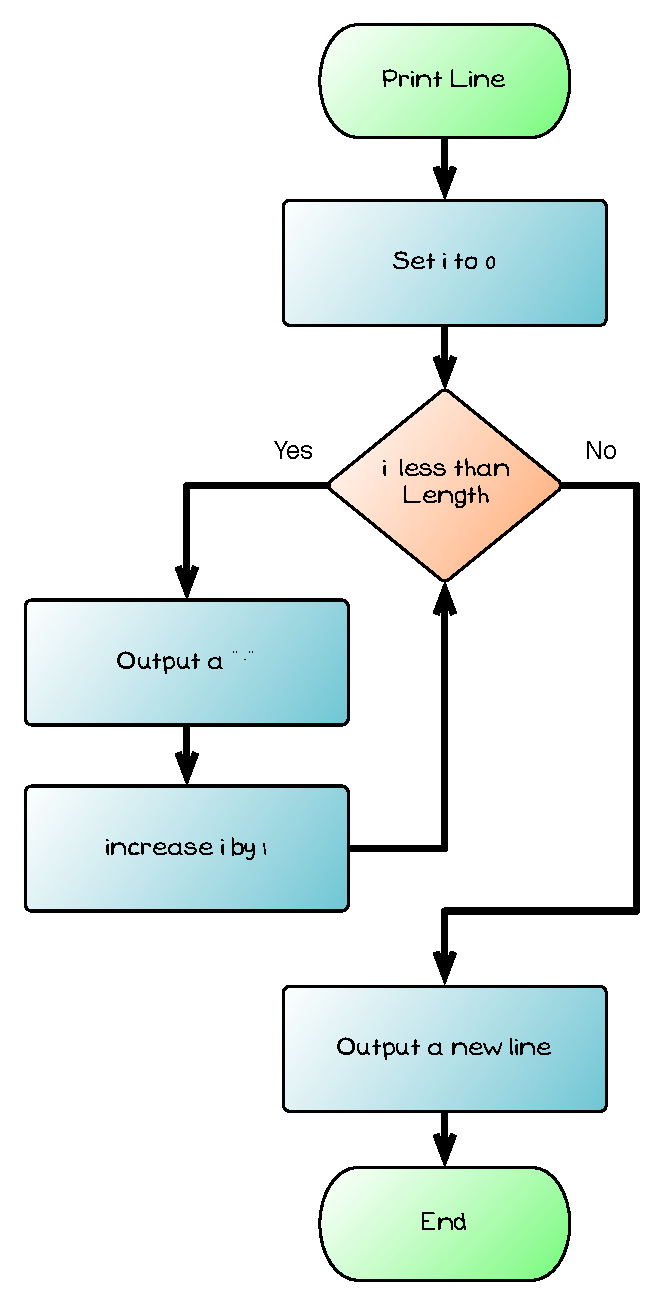
\includegraphics[width=0.37\textwidth]{./topics/control-flow/diagrams/PrintLine} 
   \caption{Flowchart for the logic in \texttt{Print Line} code}
   \label{fig:print-line}
\end{figure}

\clearpage

\begin{figure}[htbp]
   \centering
   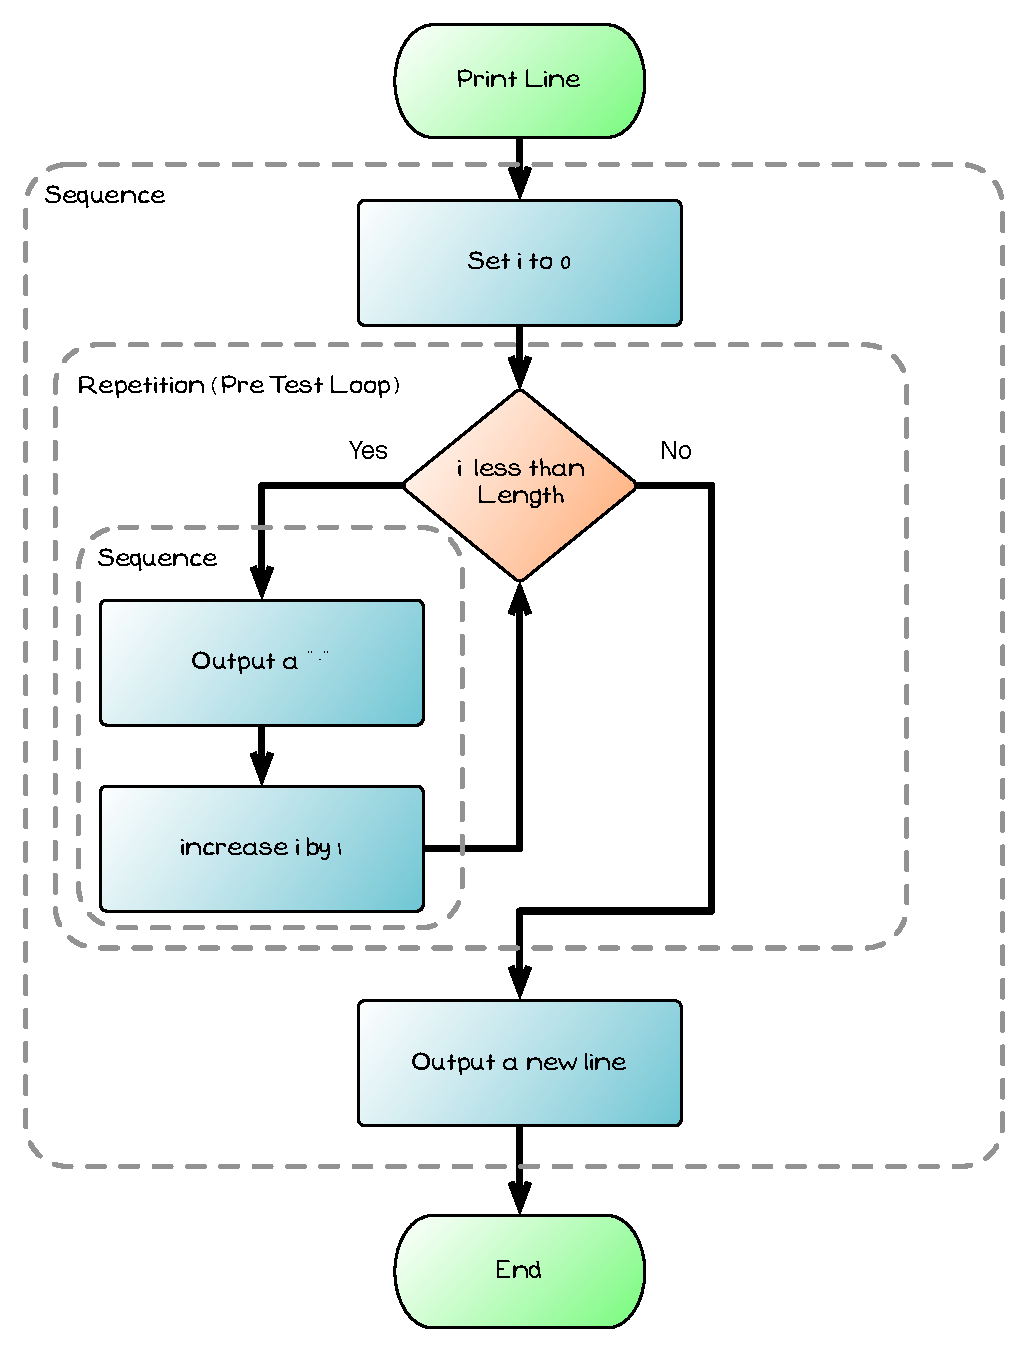
\includegraphics[width=0.57\textwidth]{./topics/control-flow/diagrams/PrintLine1} 
   \caption{Blocks in the \texttt{Print Line} code}
   \label{fig:print-line-diag-1}
\end{figure}

\pseudocode{plst:print_line}{Pseudocode for \texttt{Print Line}}{topics/control-flow/application/PrintLine.txt}

\mynote{
\begin{itemize}
  \item This code includes a \nameref{sub:local_variable} \texttt{i}.
  \item \texttt{i} is used to count the number of times the loop has executed, allowing it to stop when it has printed enough dashes.
  \item This uses a \nameref{sub:pre_test_loop}. This makes sure that no characters are printed if the length is less than or equal to zero.
  \item Notice that a sequence can be placed within a loop.
\end{itemize}
}


% subsection designing_control_flow_for_print_line (end)

\clearpage
\subsection{Designing the Control Flow for Main} % (fold)
\label{sub:designing_the_control_flow_for_main}

The last Procedure is \texttt{Main}. This is responsible for coordinating the actions of the program. It will call \texttt{Play Game} in a loop that repeatedly plays the game until the user decides to quit. \texttt{Main} will have one local variable called \texttt{again}. This will store a character, and will be used to store the value read from the user's response to the `\emph{play again}' prompt.

\begin{figure}[htbp]
   \centering
   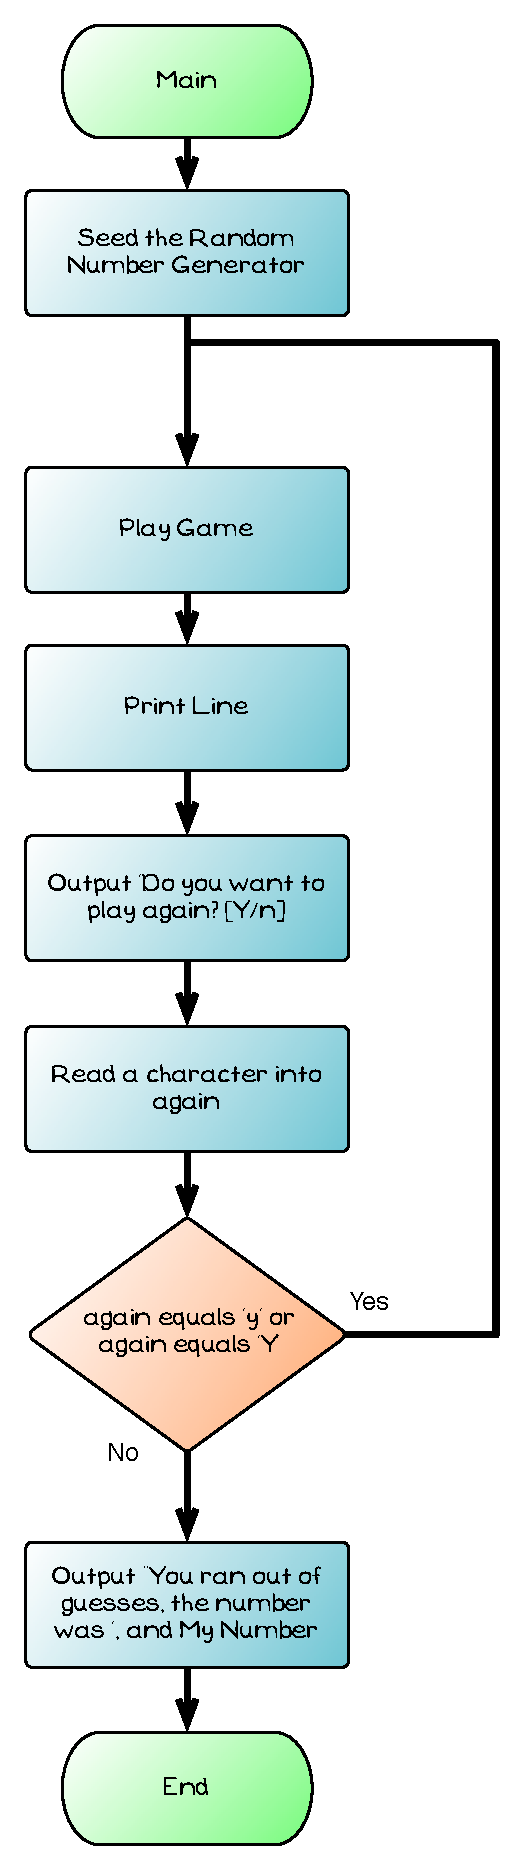
\includegraphics[width=0.31\textwidth]{./topics/control-flow/diagrams/Main} 
   \caption{Flowchart for the \texttt{Main} Procedure}
   \label{fig:main}
\end{figure}

\clearpage

\begin{figure}[htbp]
   \centering
   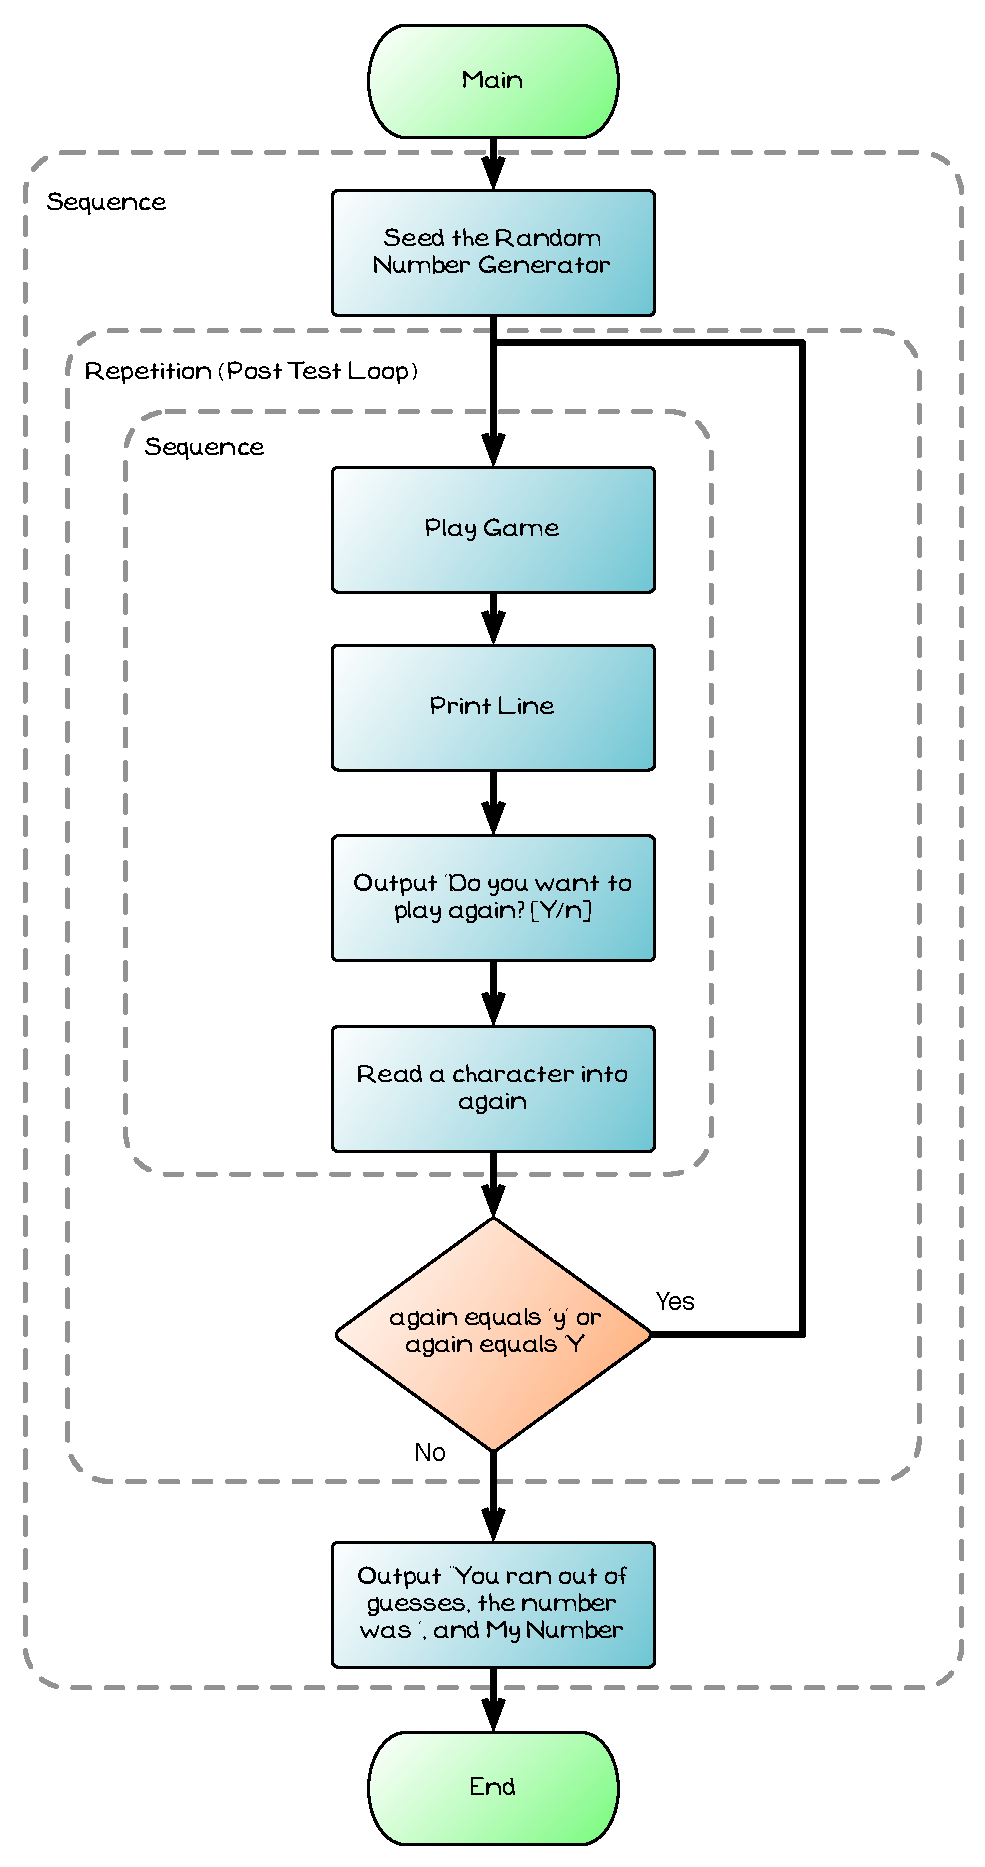
\includegraphics[width=0.55\textwidth]{./topics/control-flow/diagrams/Main1} 
   \caption{Blocks in the \texttt{Main} code}
   \label{fig:main-1}
\end{figure}

\mynote{
Computers cannot generate truly random numbers. Instead it uses a numeric sequence that appears to be random. Seeding the generator with the current time ensures that this random sequence starts at a different value each time the program is run. 
}

% subsection designing_the_control_flow_for_main (end)

\clearpage

\subsection{Writing the Code for Guess That Number} % (fold)
\label{sub:writing_the_code_for_guess_that_number}

Flowcharts and Pseudocode communicate the same ideas. They describe the actions that need to be performed within your code. The following two sections, \sref{sec:control_flow_in_c} \nameref{sec:control_flow_in_c} and  \sref{sec:control_flow_in_pascal} \nameref{sec:control_flow_in_pascal}, contain a description of the syntax needed to code these control flow statements in the C and Pascal programming languages.

\mynote{
Remember the basic process for reading the Syntax Diagrams is to:
\begin{enumerate}
  \item Find the page with the Syntax rule you are interested in knowing about.
  \item Have a quick look at the Syntax Diagram and the rules it contains. Read each rule, and get a basic feel for how it is going to come together for your program.
  \item Read the example to see one way of using the Rule. The Syntax Diagram can be used to create any number of variations of the rule, the example gives you at least one way these rules can be coded.
  \item Return to the diagram and make sure you can match each part of the example back to the rule that created it.
  \item Look up any related rules that are not explained on this rule's page.
\end{enumerate}
}

% subsection writing_the_code_for_guess_that_number (end)

\subsection{Compiling and Running Guess that Number} % (fold)
\label{sub:compiling_and_running_guess_that_number}

Once you have completed the code for this program you need to compile and run it. As this uses random numbers you cannot generate standard test data in order to check the execution. Instead you should perform a number of executions and test the different paths through the program. The main condition you want to check are:
\begin{itemize}
  \item Test failing to get the number in seven guesses.
  \item Test getting the number correct within seven guesses.
  \item Check the output messages when your guess is less than the number (you can enter a guess below 0).
  \item Check the output message when your guess is larger than the number (you can enter a guess larger than 100).
  \item Check that the random sequence is different each time, if its not make sure you have seeded the random number generator.
\end{itemize}



% subsection compiling_and_running_guess_that_number (end)

% section using_these_concepts (end)

% =============
% = C Section =
% =============
\clearpage
\def\pageLang{c}
\section{Control Flow in C} % (fold)
\label{sec:control_flow_in_c}

\subsection{Implementing the Guess that Number in C} % (fold)
\label{sub:c_guessing_game}

\sref{sec:control_flow_using_these_concepts} of this Chapter introduced the `Guess that Number' program. This program contained a Function to \texttt{Perform Guess} and Procedures to \texttt{Print Line} and \texttt{Play Game}. Each of these involved some control flow in their logic, as shown in the Flowcharts in \sref{sec:control_flow_using_these_concepts}. The full C implementation of the Guess that Number program is shown in \lref{lst:storing-data-c-guessing-game}.

\straightcode{\ccode{lst:storing-data-c-guessing-game}{C code for the Guessing Game}{code/c/control-flow/guess-that-number.c}}

\mynote{
\begin{itemize}
  \item \texttt{stdlib.h} is needed for the \texttt{random} function and the \texttt{srandom} procedure.
  \item \texttt{time.h} is needed to get the current time used to seed the random number generator.
  \item \texttt{stdbool.h} gives access to the \texttt{bool} data type in C for \nameref{sub:boolean_data}.
  \item In this code \texttt{perform\_guess} is laid out differently to that shown previously. This is also an acceptable layout as it shows the different paths clearly. While it does not show the structure as well, it is a clean and neat way of presenting this code.
\end{itemize}
}

% subsection c_guessing_game (end)


\clearpage
\subsection{C Boolean Data} % (fold)
\label{sub:c_boolean_data}

C has very flexible support for Boolean values. In C a \texttt{0} value is considered to be false, and any other value is true. Modern C compilers have now added support for an explicit Boolean type, \texttt{bool}. This type requires the \texttt{stdbool.h} header file, which defines the \texttt{bool} type as well as the values \texttt{true} and \texttt{false}.

\begin{table}[h] 
\begin{minipage}{\textwidth}
\centering
\begin{tabular}{|l|c|c|}
\hline
\multicolumn{3}{|c|}{\textbf{Boolean Type}} \\
\hline
\emph{Name} & \emph{Size} & \emph{Values} \\
\hline
\texttt{bool} & 1 byte/8 bits & \texttt{true} or \texttt{false} \\
\hline
\end{tabular}
\caption{C Boolean Type}\label{tbl:c-boolean}
\end{minipage}
\end{table}

\begin{table}[h]
  \centering
  \begin{tabular}{|c|c|c|}
    \hline
     & \textbf{Description} & \textbf{C} \\
    \hline
    \textbf{Equal} & Are the values the same? & \texttt{a == b} \\
    \hline
    \textbf{Not Equal} & Are the values different? & \texttt{a != b} \\
    \hline
    \textbf{Larger Than} & Is the left value larger than the right? & \texttt{a > b}  \\
    \hline
    \textbf{Less Than} & Is the left value smaller than the right? & \texttt{a < b}  \\
    \hline
    \textbf{Larger Or Equal} & Is the left value equal or larger than the right? & \texttt{a >= b}  \\
    \hline
    \textbf{Less Or Equal} & Is the left value smaller or equal to the right? & \texttt{a <= b}  \\
    \hline
  \end{tabular}
  \caption{C Comparison Operators}
  \label{tbl:c_comparison_op}
\end{table}

\begin{table}[h]
  \centering
  \begin{tabular}{|c|c|c|}
    \hline
     & \textbf{Description} & \textbf{C} \\
    \hline
    \textbf{And} & Are both values True? & \texttt{a \&\& b} \\
    \hline
    \textbf{Or} & Is at least one value True? & \texttt{a || b} \\
    \hline
    \textbf{Xor} & Is one value True, and the other False? & \texttt{a \^{} b} \\
    \hline
    \textbf{Not} & Is the value False? & \texttt{!a} \\
    \hline
  \end{tabular}
  \caption{Logical Operators}
  \label{tbl:c-logical-operators}
\end{table}

\mynote{
\begin{itemize}
  \item To use the Boolean type in C you must include the \texttt{stdbool.h} header.
  \item In C false is the value \texttt{0}, and true is any other value.
  \item The \texttt{stdbool.h} header gives you access to two value, \texttt{true} and \texttt{false}. \texttt{true} has the value 1, \texttt{false} has the value 0.
\end{itemize}
}

\clearpage

\csection{\ccode{clst:bool-test}{C Boolean Test Code}{code/c/control-flow/test-bools.c}}


% subsection c_boolean_data (end)
\clearpage
\subsection{C Statement (with loops)} % (fold)
\label{sub:c_statement_with_loops_}

In addition to the \nameref{sub:procedure call} and \nameref{sub:assignment_statement}, C Statements may be  \nameref{sub:branching}, \nameref{sub:looping}, or \nameref{sub:jump} Statements.

\csyntax{csynt:looping-statement}{a Statement (with branches and loops)}{looping/statement-with-loops}

\mynote{
\begin{itemize}
  \item See the following diagrams for details on this syntax:
  \begin{itemize}
    \item \nameref{sub:c_if_statement}: for the syntax of an \nameref{sub:if_statement}.
    \item \nameref{sub:c_case_statement}: for the syntax of an \nameref{sub:case_statement}.
    \item \nameref{sub:c_while_loop}: for the syntax of an \nameref{sub:pre_test_loop}.
    \item \nameref{sub:c_do_while_loop}: for the syntax of an \nameref{sub:post_test_loop}.
    \item \nameref{sub:jump_statements}: for the \nameref{sub:jump} Statements.
  \end{itemize}
  \item These statements can be coded within Functions, Procedures, and programs.
\end{itemize}
}

% subsection c_statement_with_loops_ (end)
\clearpage
\subsection{C If Statement} % (fold)
\label{sub:c_if_statement}

The if statement is a \nameref{sub:branching} statement. This can be used to optionally run a block of code, providing two alternate paths controlled by a Boolean expression.

\csyntax{csynt:branching-if-statement}{an If Statement}{branching/if-statement}

\csection{\ccode{clst-test-if}{C if test code}{code/c/control-flow/test-if.c}}

\mynote{
\begin{itemize}
  \item This is the C syntax for the \nameref{sub:if_statement}.
  \item The parenthesis surround the expression. This enables the compiler to tell where the expression ends.
  \item Notice that the \texttt{else} branch is optional.
  \item When the expression is \texttt{false} (0 in C), the else branch is taken.
  \item For any other value the first path is taken.
  \item You only need to include \texttt{stdbool.h} if you want to use the \texttt{bool} type and the values \texttt{true} or \texttt{false}.
\end{itemize}
}

% subsection c_if_statement (end)
\clearpage
\subsection{C Case Statement} % (fold)
\label{sub:c_case_statement}

The case statement allows you to switch between a number of paths.

\csyntax{csynt:branching-case-statement}{a Case Statement}{branching/case-statement}

\mynote{
\begin{itemize}
  \item This is the C syntax to declare a \nameref{sub:case_statement}.
  \item The \emph{constant expressions} in each \emph{case} must be ordinal values (integers or characters).
  \item The code in \lref{clst-test-case} shows an example use for a case statement.
  \item The \texttt{default} path is taken when none of the other paths match the expression.
  \item If the \texttt{break} is left off the end of a \emph{case} then execution will continue into the next \emph{case}. For example, in \lref{clst-simple-case} if the user enters `c' the output will be `\texttt{C and D}'
  \item Each \emph{case} can contain a number of Statements.
  \item Watch \url{http://www.youtube.com/watch?v=zIV4poUZAQo} for important details on the legendary Knights of Ni.
\end{itemize}
}

\csection{\ccode{clst-simple-case}{C case test code with a character}{code/c/control-flow/simple-case.c}}

\clearpage

\csection{\ccode{clst-test-case}{C case test code with an integer}{code/c/control-flow/test-case.c}}

% subsection case_statement (end)
\clearpage
\subsection{C Compound Statement} % (fold)
\label{sub:c_compound_statement}

Most of the C structured statements only allow single statements within each path. For example, the paths in the two branches of an \nameref{sub:c_if_statement} can only contain a single statement. The \nameref{sub:compound_statement} allows you to group together multiple statements within a single \emph{compound statement}.

\csyntax{csynt:branching-compound-statement}{a Compound Statement}{branching/compound-statement}

\csection{\ccode{clst-test-compound}{C compound statement test code}{code/c/control-flow/test-compound.c}}

\mynote{
\begin{itemize}
  \item \fref{csynt:branching-compound-statement} shows the syntax for a \nameref{sub:compound_statement} in C.
  \item The code in \lref{clst-test-compound} shows an if statement that includes two compound statements within its branches.
  \item Compound statements in C are marked with curly brackets, `\{' for the start, and `\}' for the end.
  \item The compound statement is a standard statement, and can be used anywhere a statement can appear. Its practice use is for grouping statements within other structured statements, and you are unlikely to find it used in any other way.
\end{itemize}
}

% subsection c_compound_statement (end)

\clearpage
\subsection{C While Loop} % (fold)
\label{sub:c_while_loop}

The while loop is C's \nameref{sub:pre_test_loop}, allowing a block to be repeated zero or more times.

\csyntax{csynt:looping-while-loop}{a While Loop}{looping/while-loop}

\csection{\ccode{clst-test-while}{C while loop test code}{code/c/control-flow/test-while.c}}

\mynote{
\begin{itemize}
  \item \fref{csynt:looping-while-loop} shows the syntax for a \nameref{sub:pre_test_loop} in C.
  \item This loop runs 0 to many times, checking the condition before executing the body of the loop.
  \item The parenthesis allow the compiler to determine where the condition ends, and the statement starts.
  \item The while loop repeats a single statement, you must use a \nameref{sub:compound_statement} to have multiple statements repeated. See \nameref{sub:c_compound_statement}.
\end{itemize}
}

% subsection c_while_loop (end)
\clearpage
\subsection{C Do While Loop} % (fold)
\label{sub:c_do_while_loop}

The do while loop is C's \nameref{sub:post_test_loop}, allowing a block to be repeated one or more times.

\csyntax{csynt:looping-do-while-loop}{a Do While Loop}{looping/do-while-loop}

\csection{\ccode{clst-test-do-while}{C do while loop test code}{code/c/control-flow/test-do-while.c}}

\mynote{
\begin{itemize}
  \item \fref{csynt:looping-do-while-loop} shows the syntax for a \nameref{sub:post_test_loop} in C.
  \item This loop runs 1 to many times, checking the condition after executing the body of the loop.
  \item The parenthesis allow the compiler to determine where the condition ends.
  \item The do while loop repeats a single statement, you must use a \nameref{sub:compound_statement} to have multiple statements repeated. See \nameref{sub:c_compound_statement}.
\end{itemize}
}


% subsection c_while_loop (end)
% \clearpage
\subsection{C For Loop} % (fold)
\label{sub:c_for_loop}

\csyntax{csynt:looping-for-loop}{a For Loop}{looping/for-loop}

% subsection c_while_loop (end)
\clearpage
\subsection{Jump Statements} % (fold)
\label{sub:jump_statements}

The jump statements allow you to exit out of another structure.

\csyntax{csynt:looping-jump-statements}{the Jump Statements}{looping/jump-statements}

\csection{\ccode{clst-test-jump}{C code demonstrating the jump statements}{code/c/control-flow/test-jump.c}}

\mynote{
\begin{itemize}
  \item \texttt{break} jumps to the end of the current loop.
  \item \texttt{contine} jumps back to the condition in the current loop.
  \item \texttt{return} ends the current Function or Procedure.
\end{itemize}
}

% subsection jump_statements (end)


% section control-flow_in_c (end)

% ===========================
% = Understanding Data Flow =
% ===========================

\clearpage
\def\pageLang{None}
\section{Understanding Control Flow} % (fold)
\label{sec:understanding_control_flow}

This Chapter has introduced new statements that can be used to control the sequence of actions the computer performs. These statements allow you to add \nameref{sub:branching} and \nameref{sub:looping} paths to your code. The flowcharts presented in \sref{sec:control_flow_using_these_concepts} are a great way of visualising the order in which the computer will execute the instructions. To help you fully understand these concepts this section will look at how these statements work within the computer.

\subsection{Understanding Branching in Perform Guess} % (fold)
\label{sub:understanding_branching_in_perform_guess}

\fref{fig:perform-guess-understanding} shows the flowchart for the \texttt{Perform Guess} that was developed in \sref{sub:designing_control_flow_for_perform_guess} on \nameref{sub:designing_control_flow_for_perform_guess}. The following sections show how the computer executes these actions. These illustrations will start at the call into \texttt{Perform Guess}, skipping the illustration of the steps that lead up to this call.

\begin{figure}[htbp]
   \centering
   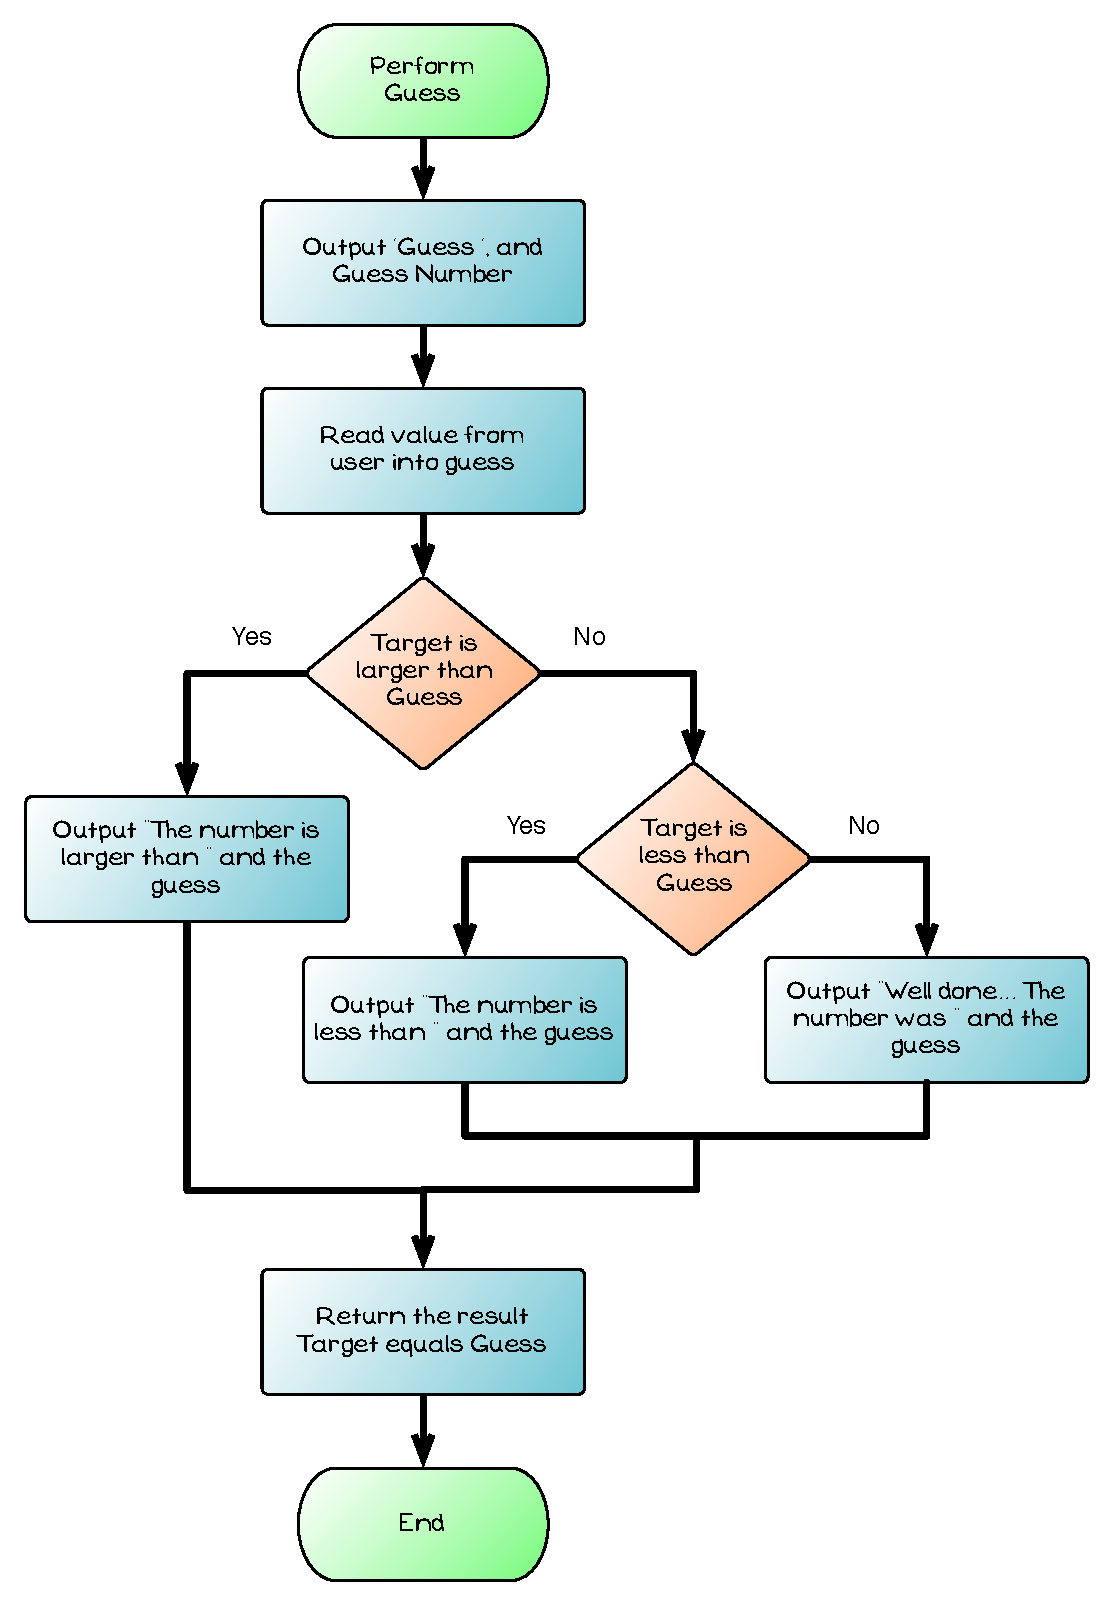
\includegraphics[width=0.5\textwidth]{./topics/control-flow/diagrams/PerformGuess5} 
   \caption{Logic for the \texttt{Perform Guess} Procedure from \fref{fig:perform-guess-5}}
   \label{fig:perform-guess-understanding}
\end{figure}

In the following illustrations \texttt{Perform Guess} will be called three times with the \texttt{target} number being \texttt{37} in each case. The following three guesses will be performed, ensuring that all paths through the flowchart are covered.
\begin{enumerate}
  \item On the first guess the user enters a guess of 50, allowing for the left most branch of this flowchart to be followed. 
  \item The second guess will be 25 to test the middle branch, taking the \emph{else} branch of the first decision and the \emph{true} branch of the second decision. 
  \item Finally the third guess will be 37, testing the right most path through the code.
\end{enumerate}


\clearpage
\subsubsection{Perform Guess is called for guess 1} % (fold)
\label{ssub:perform_guess_is_called_for_the_first_time}

In the Guess that Number program, the \texttt{Perform Guess} function is responsible for reading in the user's guess and giving them feedback. \fref{fig:perform-guess-1} shows the \texttt{Perform Guess} code being called for the first time, it is passed 1 to its \texttt{num guess} parameter and 37 to its \texttt{target} parameter.

\begin{figure}[htbp]
   \centering
   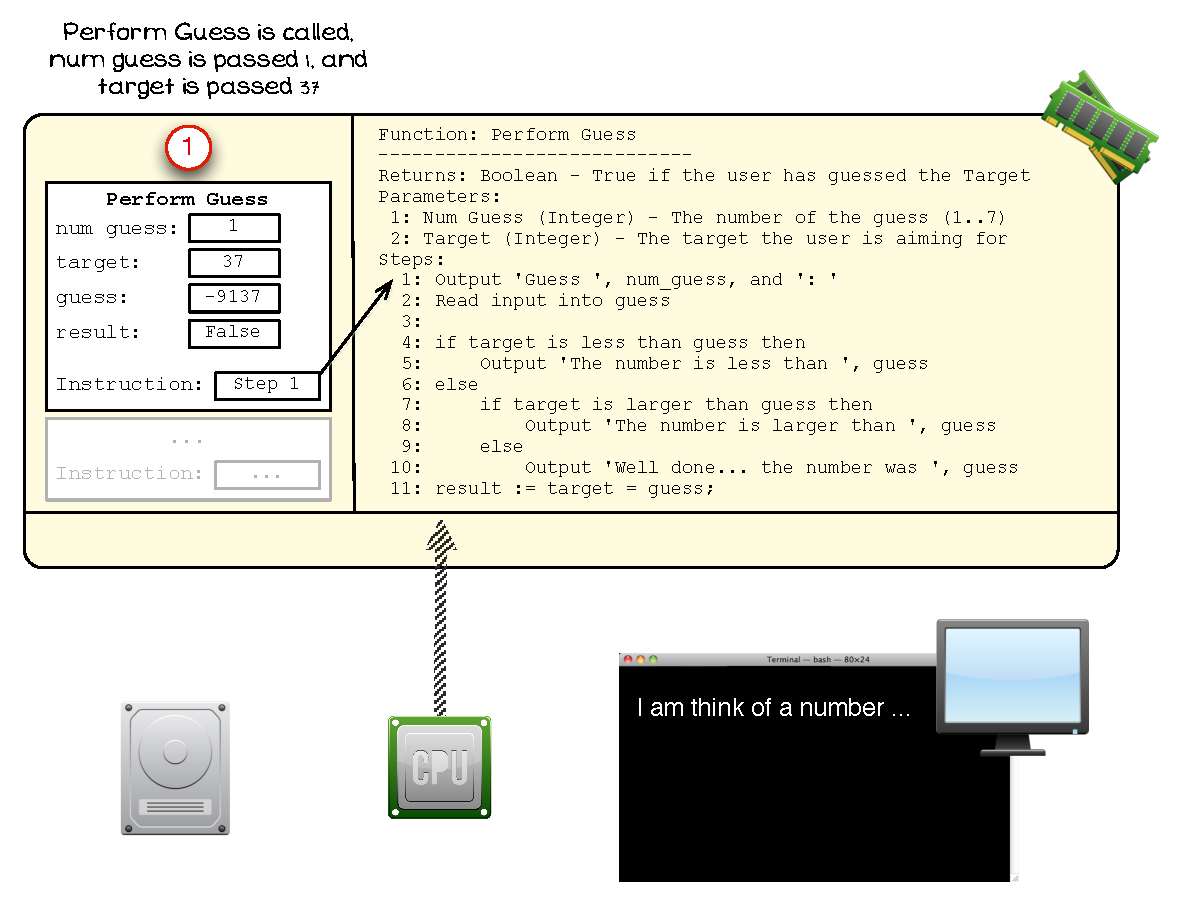
\includegraphics[width=\textwidth]{./topics/control-flow/images/PerformGuess1} 
   \caption{Perform Guess is called for the first time}
   \label{fig:perform-guess-1}
\end{figure}

\mynote{
\begin{itemize}
  \item In \fref{fig:perform-guess-1} the indicated areas show the following:
  \begin{enumerate}
    \item \texttt{Perform Guess} is called, with 1 being passed to \texttt{num guess} and 37 passed to \texttt{target}.
  \end{enumerate}
  \medskip
  \item At this point the previous code would have output `I am thinking of a number \ldots' to the Terminal.
  \item The values in \texttt{guess} and \texttt{result} have not been initialised, so they have whatever value was in that memory location previously.
\end{itemize}
}

% subsubsection perform_guess_is_called_for_the_first_time (end)
\clearpage
\subsubsection{Execution reaches the if branch for guess 1} % (fold)
\label{ssub:execution_reaches_the_if_branch}

Execution of \texttt{Perform Guess} occurs as normal, each instruction is run one after the other.

\begin{figure}[htbp]
   \centering
   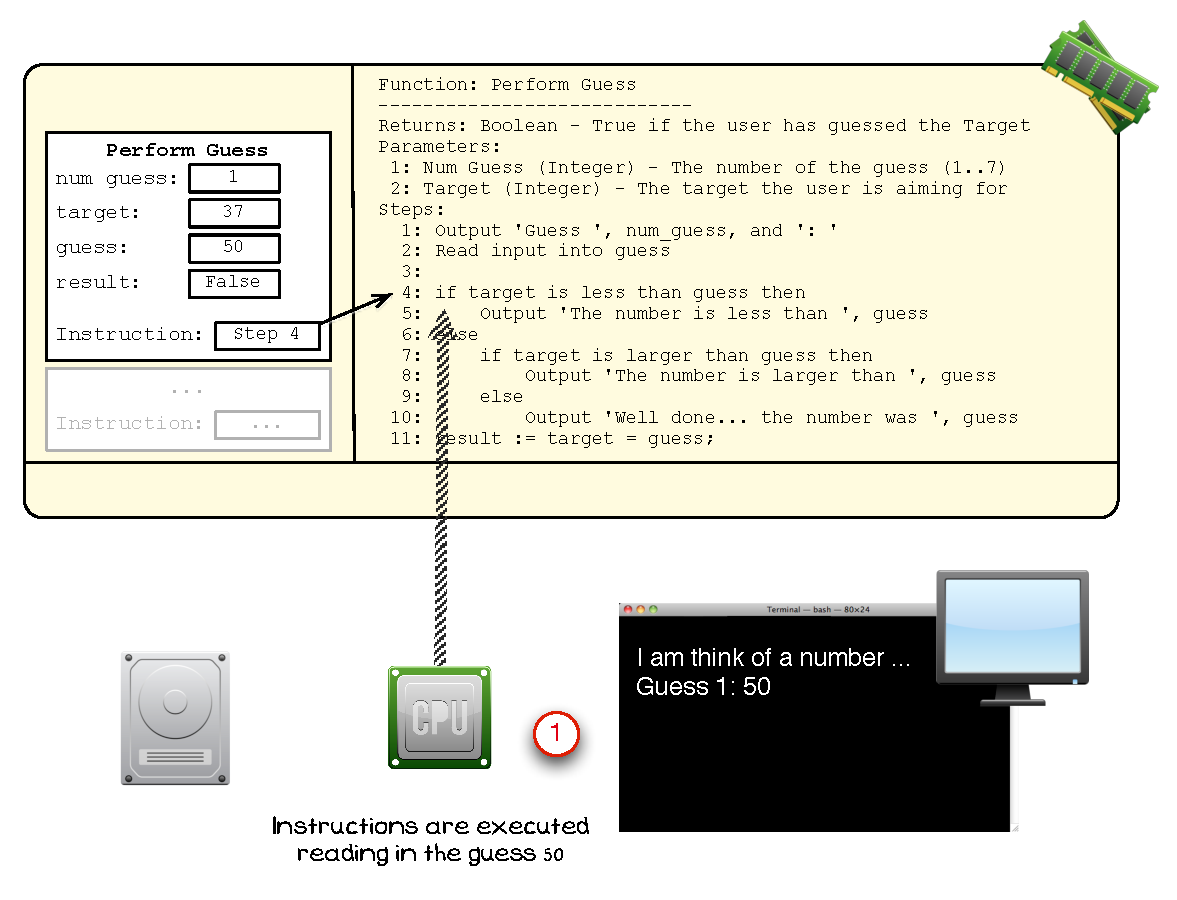
\includegraphics[width=\textwidth]{./topics/control-flow/images/PerformGuess2} 
   \caption{Program's steps are executed up to step 4}
   \label{fig:perform-guess-2}
\end{figure}

\mynote{
\begin{itemize}
  \item In \fref{fig:perform-guess-2} the indicated areas show the following:
  \begin{enumerate}
    \item Execution proceeds one instruction at a time up to the \nameref{sub:if_statement} at step 4.
  \end{enumerate}
  \medskip
  \item These steps output a prompt (step 1), and read in a response (step 2).
  \item Step 2 reads a the user's response into the \texttt{guess} variable.
  \item When the computer executes step 4 it evaluates the \nameref{sub:if_statement}'s expression and then selectively runs one of the two available paths.
\end{itemize}
}

% subsubsection execution_reaches_the_if_branch (end)
\clearpage
\subsubsection{If takes the True branch for guess 1} % (fold)
\label{ssub:if_takes_the_true_branch_for_guess_1}

With the first guess the expression in the \nameref{sub:if_statement} is \texttt{true}, \texttt{target} \textbf{is} less than \texttt{guess}. The computer jumps into the \emph{true} branch of the if statement. 

\begin{figure}[htbp]
   \centering
   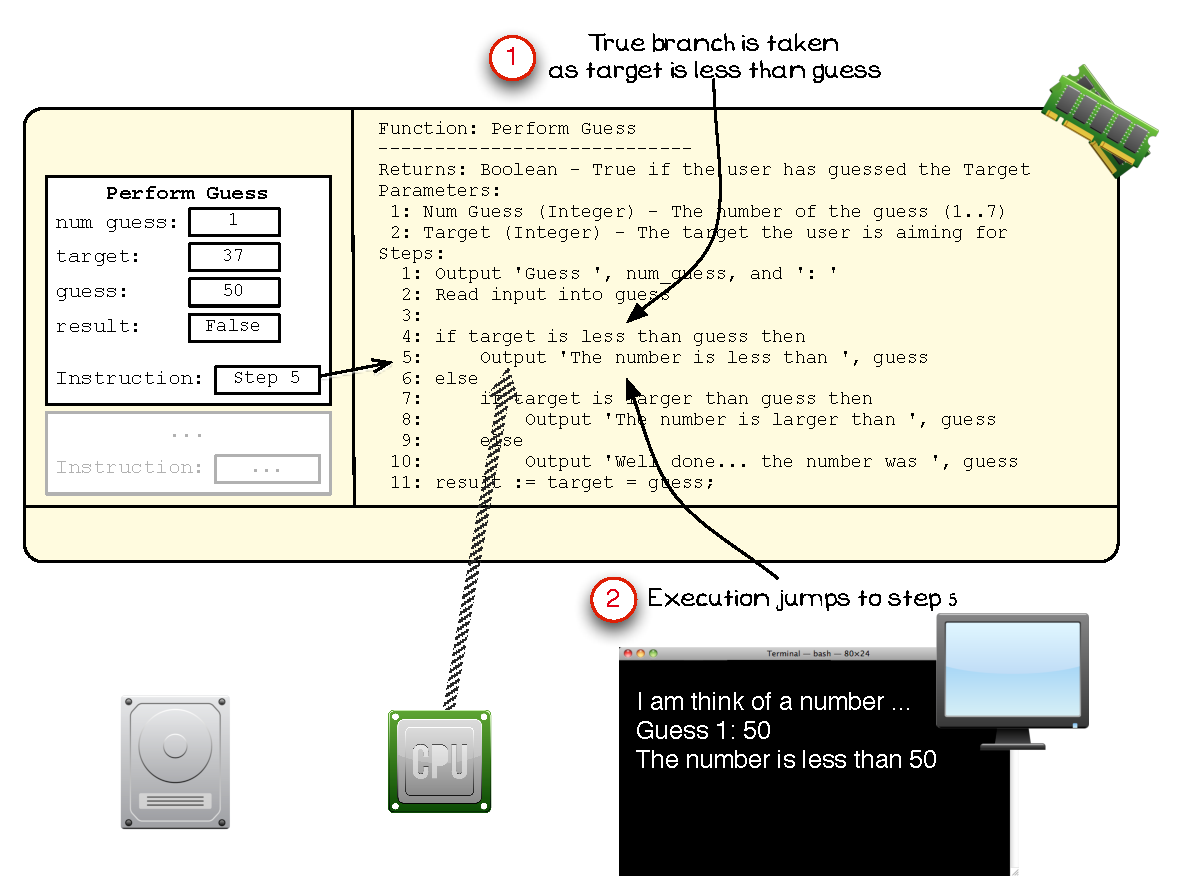
\includegraphics[width=\textwidth]{./topics/control-flow/images/PerformGuess3} 
   \caption{The \emph{true} branch is taken as \texttt{target} is less than \texttt{guess}}
   \label{fig:perform-guess-3}
\end{figure}

\mynote{
\begin{itemize}
  \item In \fref{fig:perform-guess-3} the indicated areas show the following:
  \begin{enumerate}
    \item \texttt{target} is less than \texttt{guess} so the \emph{true} branch is executed.
    \item This means the code jumps to step 5.
  \end{enumerate}
  \medskip
  \item Step 5 outputs `The number is less than 50' to the Terminal.
\end{itemize}
}

% subsubsection if_takes_the_true_branch_for_guess_1 (end)
\clearpage

\subsubsection{Control jumps to the end of \texttt{Perform Guess} for guess 1} % (fold)
\label{ssub:control_jumps_to_step_11_for_guess_1}

Once step 5 finishes, control jumps to step 11, skipping the \emph{else} branch of the if statement from step 4.

\begin{figure}[htbp]
   \centering
   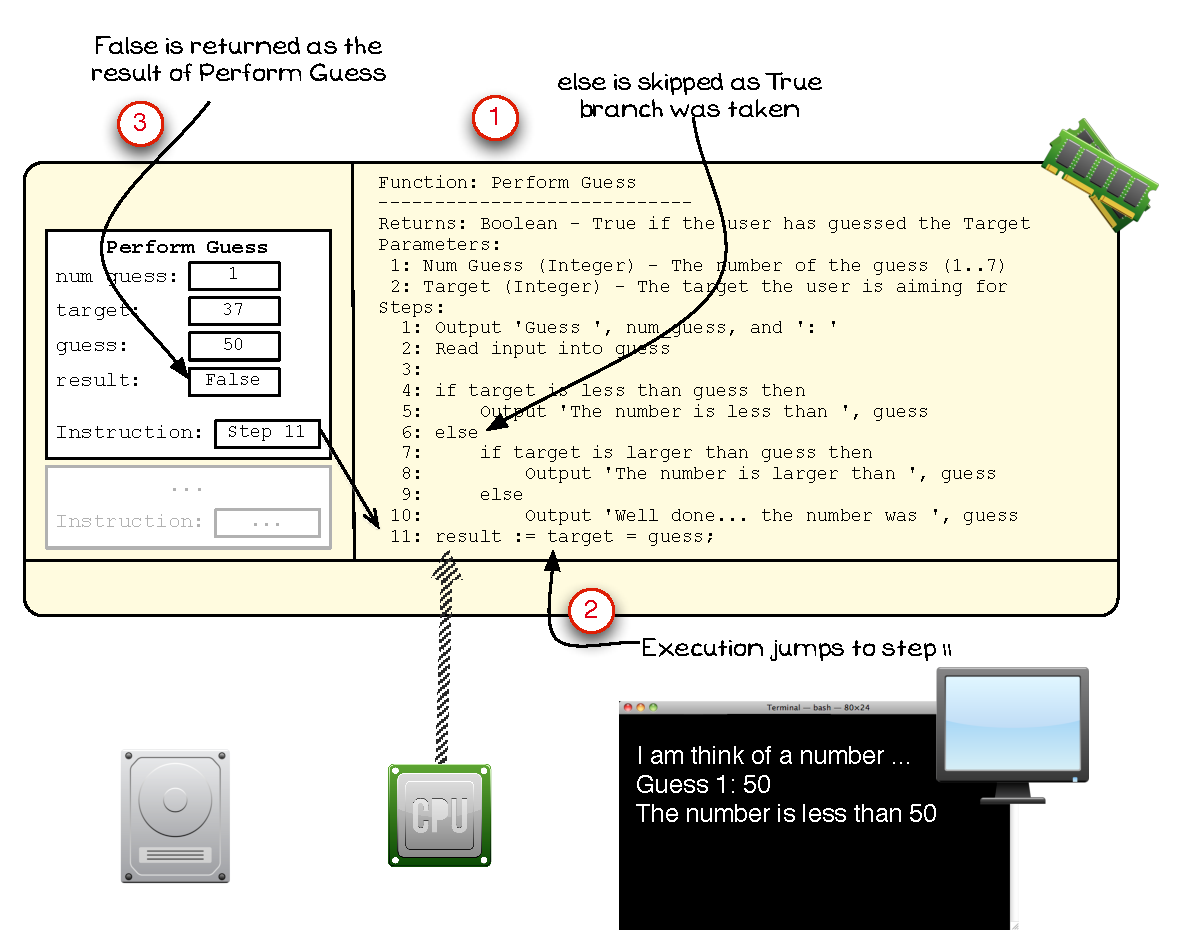
\includegraphics[width=\textwidth]{./topics/control-flow/images/PerformGuess4} 
   \caption{\texttt{Perform Guess} finishes for guess 1, returning the result \texttt{false}}
   \label{fig:perform-guess-4}
\end{figure}

\mynote{
\begin{itemize}
  \item In \fref{fig:perform-guess-4} the indicated areas show the following:
  \begin{enumerate}
    \item Steps 6 to 10 are skipped as the \emph{true} branch was taken.
    \item The next instruction is therefore step 11.
    \item This evaluates the expression \texttt{target} \textbf{equals} \texttt{guess}, which is \texttt{false}.
  \end{enumerate}
\end{itemize}
}

% subsubsection control_jumps_to_step_11_for_guess_1 (end)
\clearpage

\subsubsection{\texttt{Perform Guess} is called again for guess 2} % (fold)
\label{ssub:perform_guess_is_called_for_guess_2}

\texttt{Perform Guess} is called again, this time it is passed 2 for \texttt{guess num} and 37 for \texttt{target}. This executes the code in \texttt{Perform Guess}, one instruction at a time, eventually reaching step 4.

\begin{figure}[htbp]
   \centering
   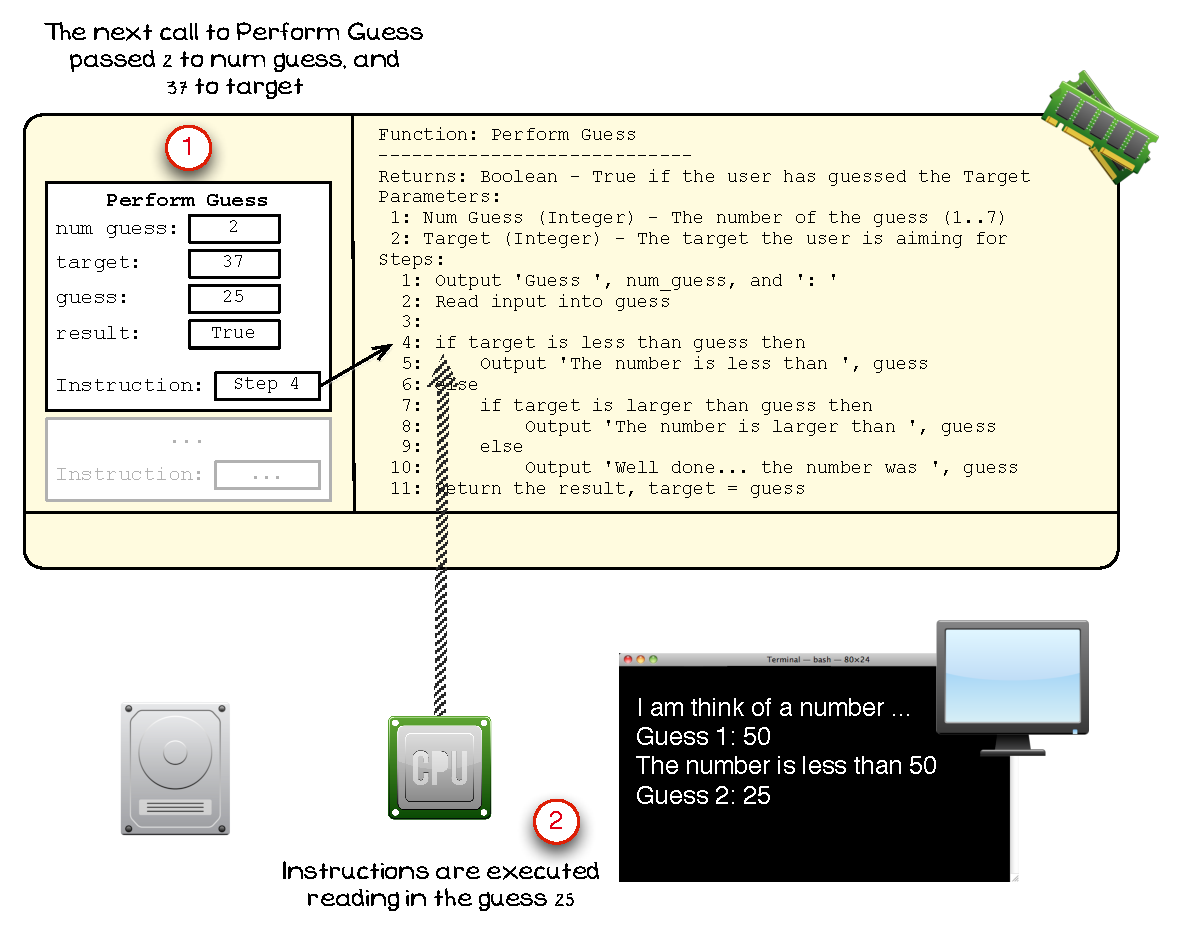
\includegraphics[width=\textwidth]{./topics/control-flow/images/PerformGuess5} 
   \caption{\texttt{Perform Guess} is run for guess 2 and advanced to step 4}
   \label{fig:perform-guess-5}
\end{figure}

\mynote{
\begin{itemize}
  \item In \fref{fig:perform-guess-5} the indicated areas show the following:
  \begin{enumerate}
    \item The call to \texttt{Perform Guess} is passed 2 for the \texttt{guess num} parameter, and 37 for the \texttt{target} parameter.
    \item The user enters 25 as their guess, this is read into the \texttt{guess} variable.
  \end{enumerate}
  \medskip
  \item The previous call ended and control returned to the caller. This is a now a new call to \texttt{Perform Guess}.
  \item Step 1 outputs a prompts for the user to enter `Guess 2: '.
  \item Step 2 reads a the user's response into the \texttt{guess} variable.
  \item When the computer executes step 4 it evaluates the \nameref{sub:if_statement}'s expression and then selectively runs one of the two available paths.
\end{itemize}
}

% subsubsection perform_guess_is_called_for_guess_2 (end)
\clearpage

\subsubsection{If takes the \emph{else} branch for guess 2} % (fold)
\label{ssub:if_takes_the_else_branch_for_guess_2}

With the second guess the expression in the \nameref{sub:if_statement} is \texttt{false}, \texttt{target} \textbf{is not} less than \texttt{guess}. The computer jumps into the \emph{else} branch of the if statement. 

\begin{figure}[htbp]
   \centering
   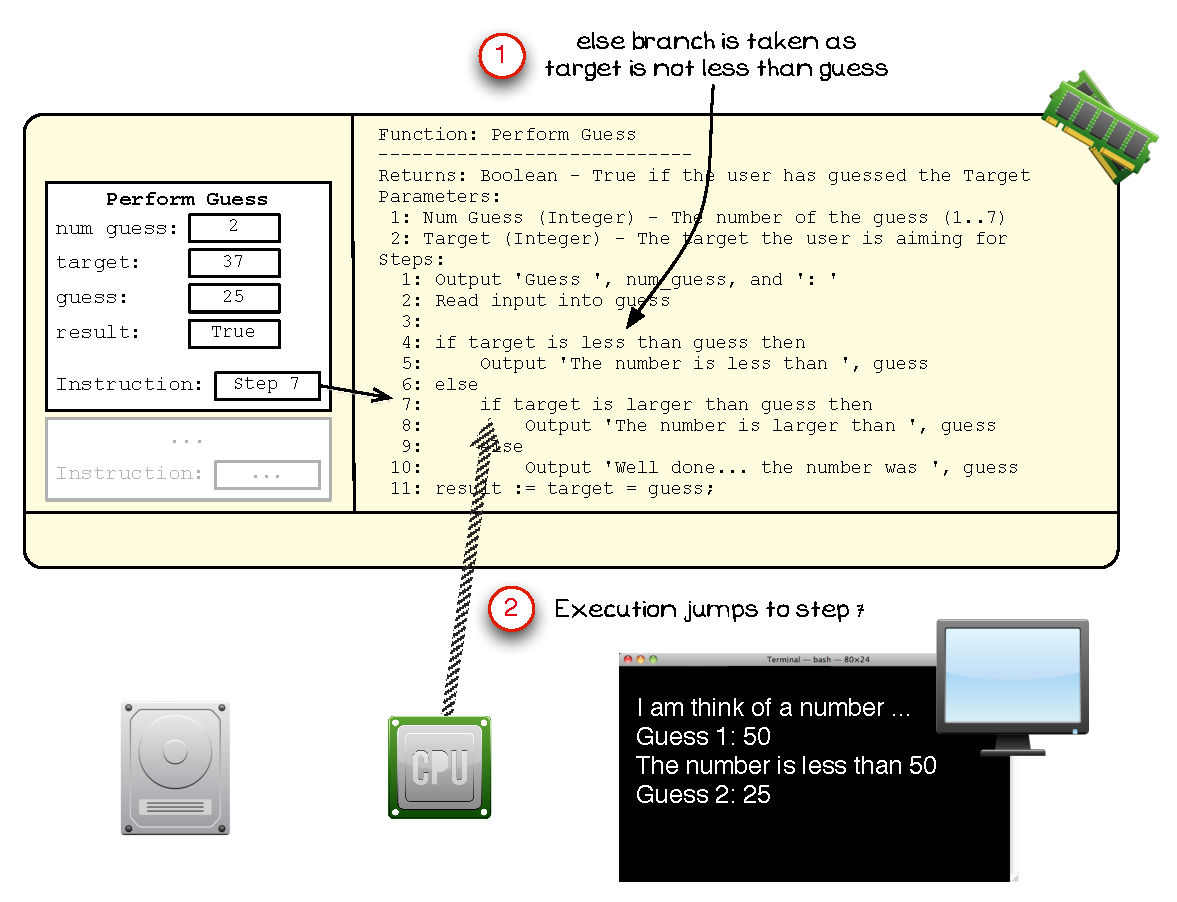
\includegraphics[width=\textwidth]{./topics/control-flow/images/PerformGuess6} 
   \caption{Control jumps to step 7 as the target is not less than the guess}
   \label{fig:perform-guess-6}
\end{figure}

\mynote{
\begin{itemize}
  \item In \fref{fig:perform-guess-6} the indicated areas show the following:
  \begin{enumerate}
    \item \texttt{target} is not less than \texttt{guess} so the \emph{else} branch is executed.
    \item This means the code jumps to step 7, skipping the \emph{true} branch.
  \end{enumerate}
  \medskip
  \item Step 7 is another \nameref{sub:if_statement}, it checks if \texttt{target} is \emph{larger} than \texttt{guess}. This expression is \texttt{true}, so it will take the \emph{true} branch next.
\end{itemize}
}

% subsubsection if_takes_the_else_branch_for_guess_2 (end)
\clearpage

\subsubsection{The inner if's \emph{true} branch is taken in guess 2} % (fold)
\label{ssub:the_inner_if_s_true_branch_is_taken_in_guess_2}

The expression in step 7 is \texttt{true}, so the if statement directs the computer into the \emph{true} branch at step 8.

\begin{figure}[htbp]
   \centering
   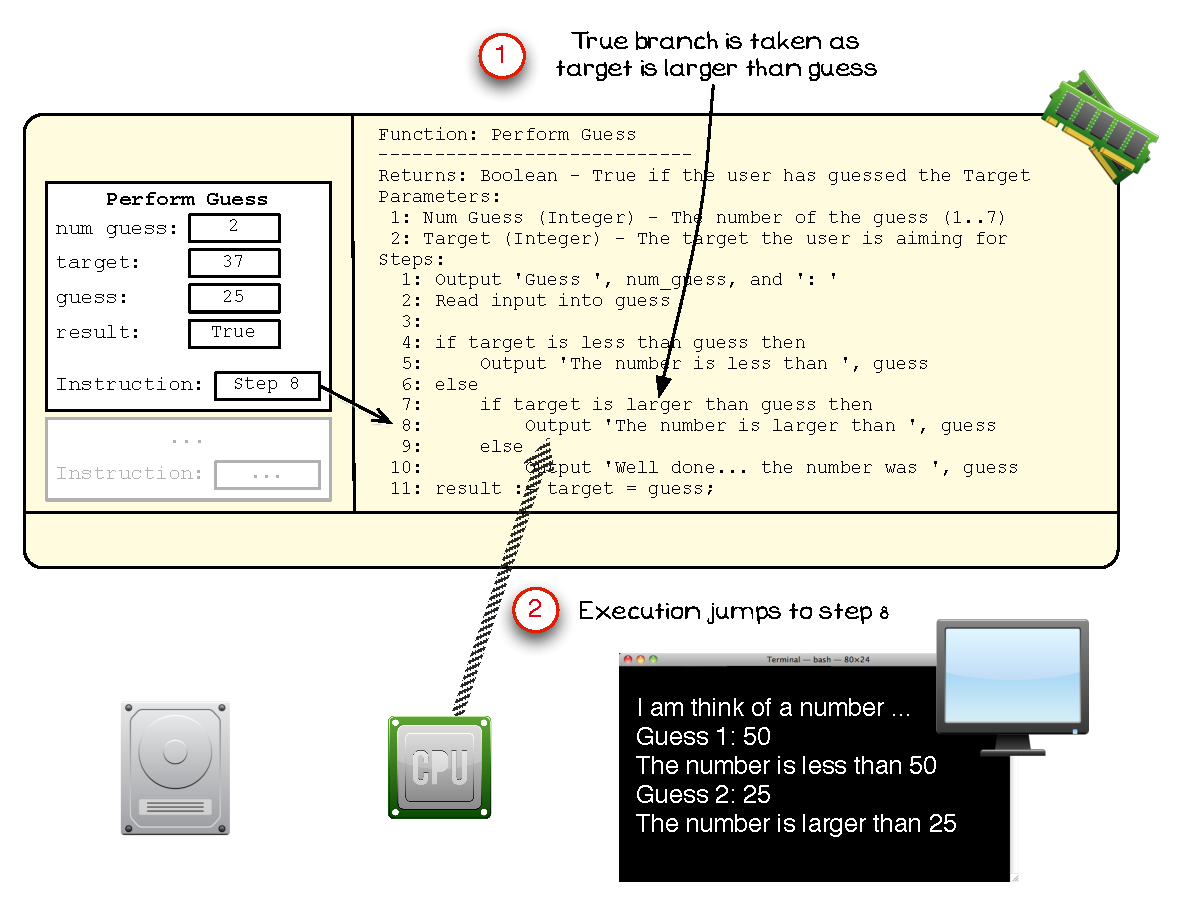
\includegraphics[width=\textwidth]{./topics/control-flow/images/PerformGuess7} 
   \caption{Control continues into the \emph{true} branch of the inner if statement}
   \label{fig:perform-guess-7}
\end{figure}

\mynote{
\begin{itemize}
  \item In \fref{fig:perform-guess-7} the indicated areas show the following:
  \begin{enumerate}
    \item \texttt{target} is larger than \texttt{guess} so the \emph{true} branch is taken.
    \item This means the code jumps to step 8.
  \end{enumerate}
  \medskip
  \item Step 8 outputs the message `The number if larger than 25' to the Terminal.
\end{itemize}
}

% subsubsection the_inner_if_s_true_branch_is_taken_in_guess_2 (end)
\clearpage

\subsubsection{Control jumps to the end of \texttt{Perform Guess} for guess 2} % (fold)
\label{ssub:control_jumps_to_step_11_for_guess_2}

Once step 8 finishes, control jumps to step 11, skipping the \emph{else} branch of the if statement from step 7 and also ending the if statement started at step 4.

\begin{figure}[htbp]
   \centering
   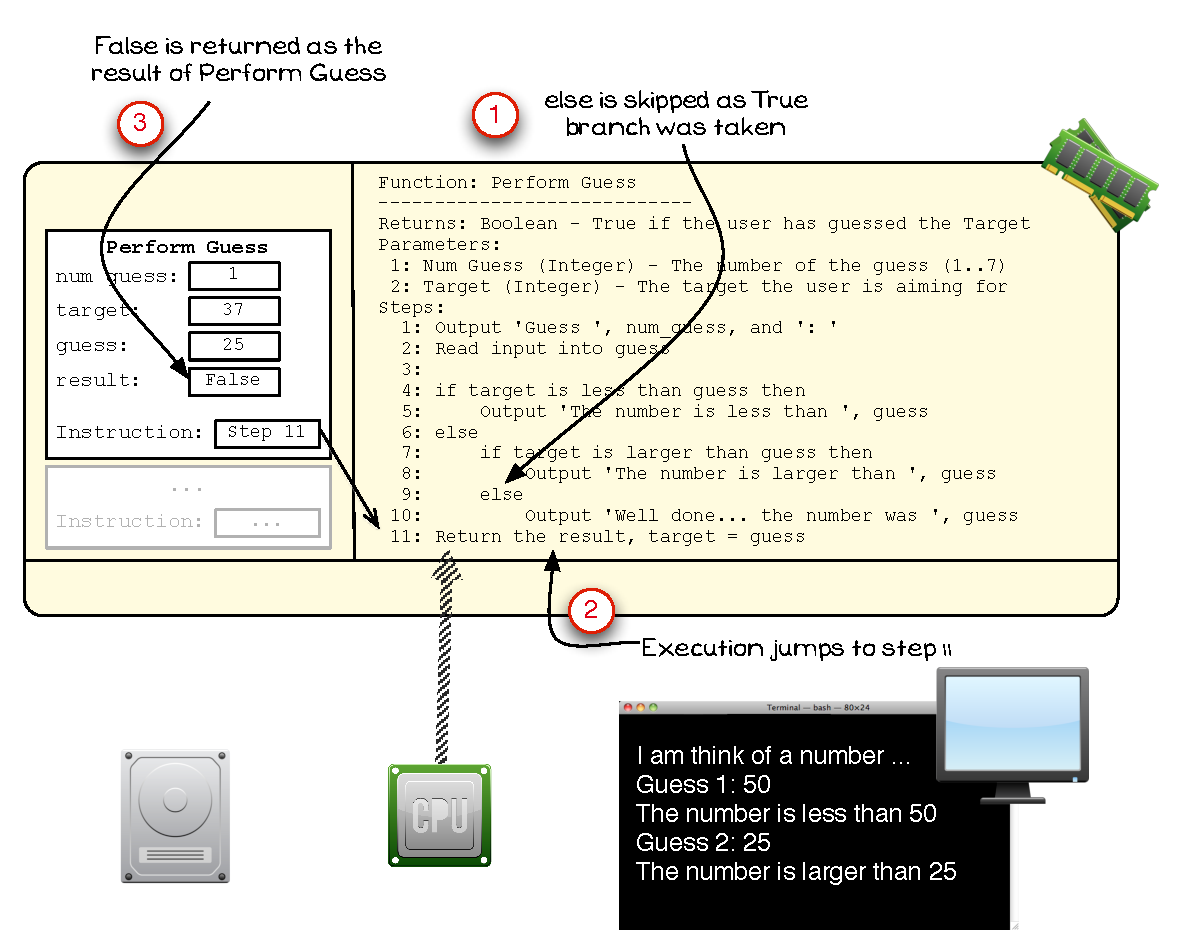
\includegraphics[width=\textwidth]{./topics/control-flow/images/PerformGuess8} 
   \caption{Guess 2 ends with \texttt{Perform Guess} returning \texttt{False}}
   \label{fig:perform-guess-8}
\end{figure}

\mynote{
\begin{itemize}
  \item In \fref{fig:perform-guess-8} the indicated areas show the following:
  \begin{enumerate}
    \item The else branch starting at step 9 is skipped as the \emph{true} branch was taken.
    \item The next instruction is therefore step 11, ending the if statements starts at steps 7 and 4.
    \item \texttt{Perform Guess} returns the result \texttt{false} as the expression \texttt{target} equals \texttt{guess} is \texttt{false}.
  \end{enumerate}
\end{itemize}
}

% subsubsection control_jumps_to_step_11_for_guess_2 (end)
\clearpage

\subsubsection{Perform Guess is called again for guess 3} % (fold)
\label{ssub:perform_guess_is_called_again_for_guess_3}

\texttt{Perform Guess} is called again, this time it is passed 3 for \texttt{guess num} and 37 for \texttt{target}. This executes the code in \texttt{Perform Guess}, one instruction at a time, eventually reaching step 4.

\begin{figure}[htbp]
   \centering
   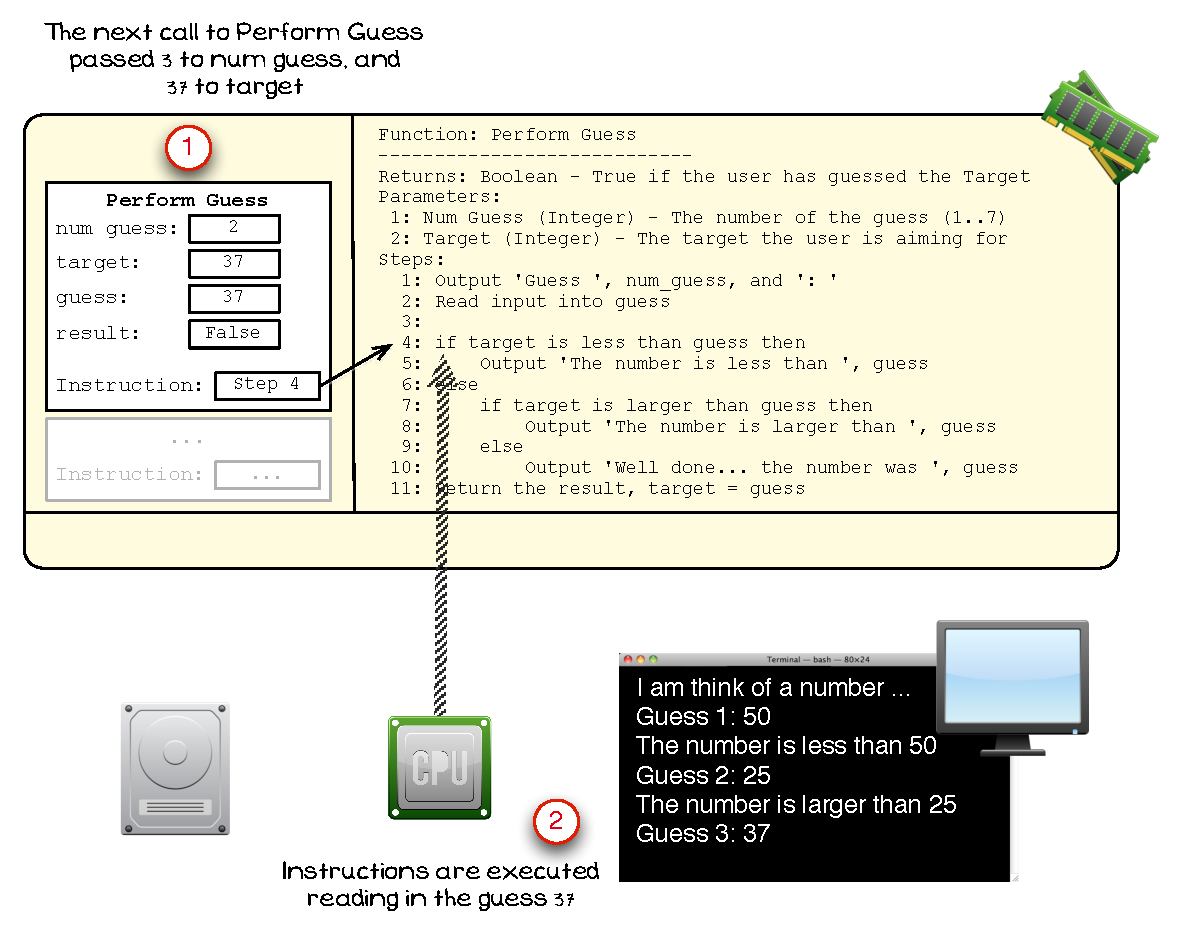
\includegraphics[width=\textwidth]{./topics/control-flow/images/PerformGuess9} 
   \caption{\texttt{Perform Guess} is run for guess 3 and advanced to step 4}
   \label{fig:perform-guess-9}
\end{figure}

\mynote{
\begin{itemize}
  \item In \fref{fig:perform-guess-9} the indicated areas show the following:
  \begin{enumerate}
    \item The call to \texttt{Perform Guess} is passed 3 for the \texttt{guess num} parameter, and 37 for the \texttt{target} parameter.
    \item The user enters 37 as their guess, this is read into the \texttt{guess} variable.
  \end{enumerate}
  \medskip
  \item The previous call ended and control returned to the caller. This is a now a new call to \texttt{Perform Guess}.
  \item Step 1 outputs a prompts for the user to enter `Guess 3: '.
  \item Step 2 reads a the user's response into the \texttt{guess} variable.
  \item When the computer executes step 4 it evaluates the \nameref{sub:if_statement}'s expression and then selectively runs one of the two available paths. In this case the expression is \texttt{false} as \texttt{target} is not less than \texttt{guess}.
\end{itemize}
}

% subsubsection perform_guess_is_called_again_for_guess_3 (end)
\clearpage

\subsubsection{If takes the \emph{else} branch for guess 3} % (fold)
\label{ssub:if_takes_the_else_branch_for_guess_3}

The \texttt{target} is \textbf{not} less than the user's guess, so the \emph{else} branch of the if statement at step 4 is taken, with the computer jumping to step 7.

\begin{figure}[htbp]
   \centering
   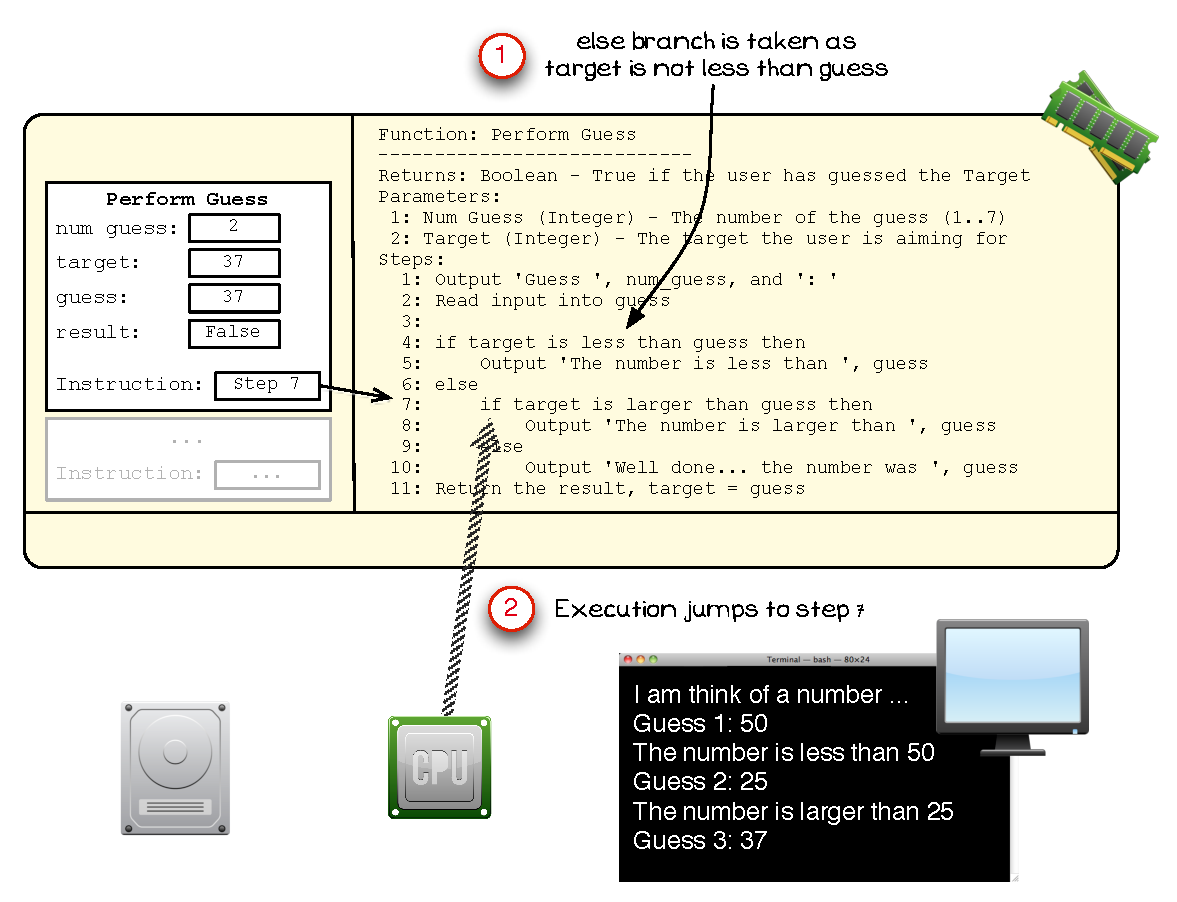
\includegraphics[width=\textwidth]{./topics/control-flow/images/PerformGuess10} 
   \caption{The \emph{else} branch is taken as \texttt{target} is not less than \texttt{guess} for guess 3}
   \label{fig:perform-guess-10}
\end{figure}

\mynote{
\begin{itemize}
  \item In \fref{fig:perform-guess-10} the indicated areas show the following:
  \begin{enumerate}
    \item \texttt{target} is not less than \texttt{guess} so the \emph{else} branch is executed.
    \item This means the code jumps to step 7, skipping the \emph{true} branch.
  \end{enumerate}
  \medskip
  \item Step 7 is another \nameref{sub:if_statement}, it checks if \texttt{target} is \emph{larger} than \texttt{guess}. This expression is also \texttt{false}, \texttt{target} is \emph{not} larger than \texttt{guess}.
\end{itemize}
}

% subsubsection if_takes_the_else_branch_for_guess_3 (end)
\clearpage

\subsubsection{The inner if's \emph{else} branch is taken in guess 3} % (fold)
\label{ssub:the_inner_if_s_else_branch_is_taken_in_guess_3}

The \texttt{target} is \textbf{not} larger than the user's guess, so the \emph{else} branch of the if statement at step 7 is taken, with the computer jumping to step 10.

\begin{figure}[htbp]
   \centering
   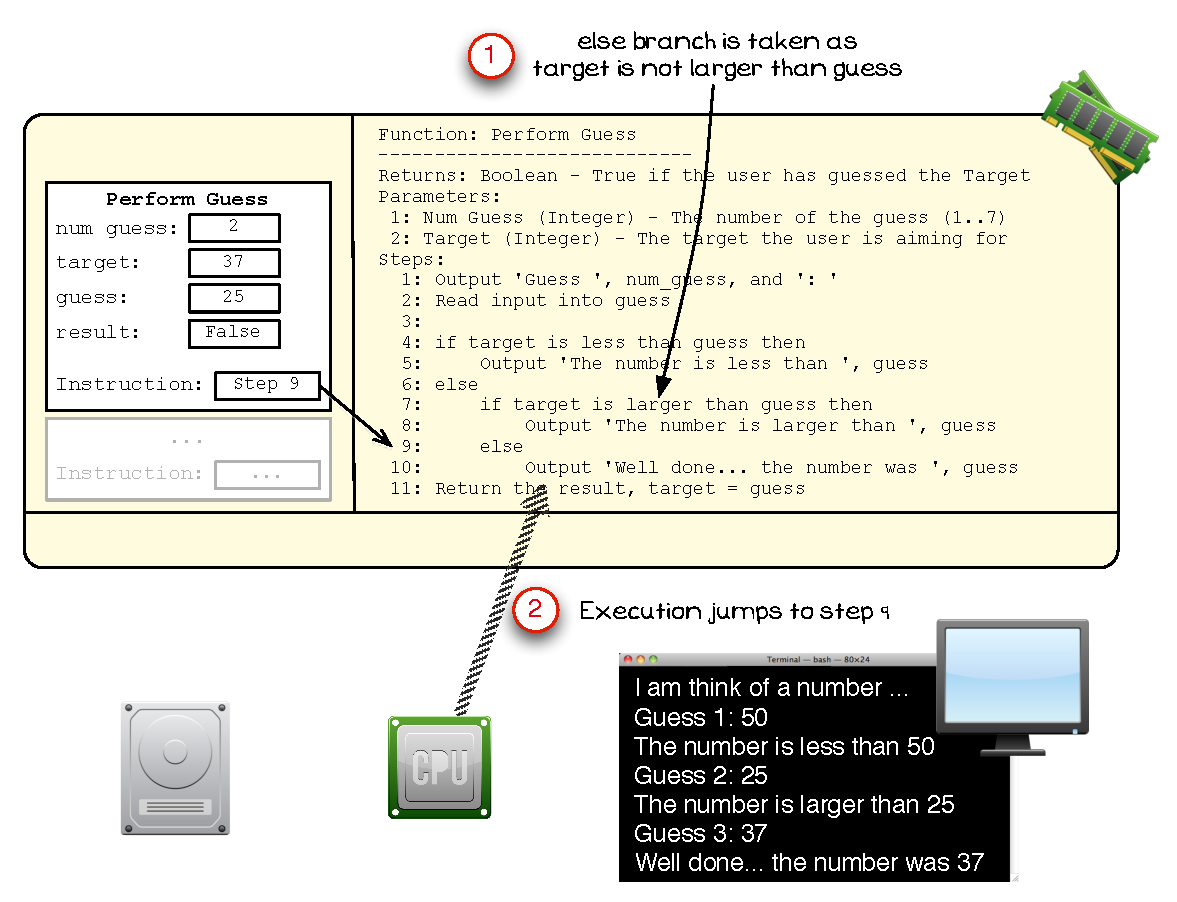
\includegraphics[width=\textwidth]{./topics/control-flow/images/PerformGuess11} 
   \caption{The \texttt{target} is not larger than \texttt{guess}, so the \emph{else} branch of the if statement at step 7 is taken.}
   \label{fig:perform-guess-11}
\end{figure}

\mynote{
\begin{itemize}
  \item In \fref{fig:perform-guess-11} the indicated areas show the following:
  \begin{enumerate}
    \item \texttt{target} is not larger than \texttt{guess} so the \emph{else} branch is executed.
    \item This means the code jumps to step 10, skipping the \emph{true} branch.
  \end{enumerate}
  \medskip
  \item Step 10 outputs `Well done\ldots the number was 37' to the Terminal.
\end{itemize}
}

% subsubsection the_inner_if_s_else_branch_is_taken_in_guess_3 (end)
\clearpage

\subsubsection{Control jumps to the end of \texttt{Perform Guess} for guess 3} % (fold)
\label{ssub:control_jumps_to_step_11_for_guess_3}

Once step 10 finishes, control jumps to step 11, ending the if statements from step 7 and step~ 4.

\begin{figure}[htbp]
   \centering
   \includegraphics[width=\textwidth]{./topics/control-flow/images/PerformGuess12} 
   \caption{Program's entry point is loaded onto the Stack}
   \label{fig:perform-guess-12}
\end{figure}

\mynote{
\begin{itemize}
  \item In \fref{fig:perform-guess-12} the indicated areas show the following:
  \begin{enumerate}
    \item The if statements at steps 7 and 4 end, with control jumping to step 11.
    \item The result returned will be \texttt{true}, \texttt{target} does equal \texttt{guess}.
  \end{enumerate}
  
\end{itemize}
}

% subsubsection control_jumps_to_step_11_for_guess_3 (end)
% subsection understanding_branching_in_perform_guess (end)

\clearpage
\subsection{Understanding Looping in Play Game} % (fold)
\label{sub:understanding_looping_in_play_game}

\fref{fig:play-game-understanding} shows the flowchart for the \texttt{Play Game} procedure that was developed in \sref{sub:designing_control_flow_for_play_game} on \nameref{sub:designing_control_flow_for_play_game}. The following sections outline how these actions are executed within the computer.

\begin{figure}[htbp]
   \centering
   \includegraphics[width=0.38\textwidth]{./topics/control-flow/diagrams/PlayGame} 
   \caption{Logic for the \texttt{Play Game} Procedure from \fref{fig:play-game}}
   \label{fig:play-game-understanding}
\end{figure}

In the following illustrations \texttt{Play Game} will be called once, and will perform three guesses. These three guesses match the calls illustrated in \sref{sub:understanding_branching_in_perform_guess} \nameref{sub:understanding_branching_in_perform_guess}. In each case the details of the call into \texttt{Perform Guess} will not be recovered, but you can refer back to the previous section if needed. 

The illustrations will show how the loop in the flowchart is handled by the computer. As this includes a \texttt{do...while}/\texttt{repeat...until} loop, the explanations will present both boolean expressions. Please ensure that you check the logic based on the implementation you will use.

\clearpage
\subsubsection{\texttt{Play Game} is called} % (fold)
\label{ssub:play game_is_called}

At some point the \texttt{Play Game} procedure is called. This will be responsible for coordinating the actions needed to play one game of Guess that Number. It will call \texttt{Perform Guess} to do the work needed to perform each individual guess.

\begin{figure}[htbp]
   \centering
   \includegraphics[width=\textwidth]{./topics/control-flow/images/PlayGame1} 
   \caption{\texttt{Play Game} is called, it is allocated space on the Stack for its local variables}
   \label{fig:play-game-1}
\end{figure}

\mynote{
\begin{itemize}
  \item In \fref{fig:play-game-1} the indicated areas show the following:
  \begin{enumerate}
    \item \texttt{Play Game} is allocated spaces on the stack for its local variables.
  \end{enumerate}
  \medskip
  \item Local variables are not initialised, so their values are whatever happened to be at that location in memory before.
  \item Step 1 generates a random number and stores this in \texttt{my num}.
  \item Step 2 initialises the value of \texttt{guess num} with the value 0.
  \item Step 3 will output a message indicating the start of the game.
\end{itemize}
}

% subsubsection play game_is_called (end)
\clearpage

\subsubsection{The loop is entered} % (fold)
\label{ssub:control_runs_to_step_4}

Steps 1 to 3 execute and initialise the \texttt{my num} and \texttt{guess num} local variables. 

\begin{figure}[htbp]
   \centering
   \includegraphics[width=\textwidth]{./topics/control-flow/images/PlayGame2} 
   \caption{}
   \label{fig:play-game-2}
\end{figure}

\mynote{
\begin{itemize}
  \item In \fref{fig:play-game-2} the indicated areas show the following:
  \begin{enumerate}
    \item Steps 1 to 3 are executed, and then control enters the repeated block.
  \end{enumerate}
  \medskip
  \item The repeated instructions will continue as normal.
  \item If this were a \nameref{sub:pre_test_loop}, the condition would be checked \emph{before} the loop body was executed. Other than that the two kinds of loops are the same.
\end{itemize}
}

\csection{Remember that in C the \nameref{sub:post_test_loop} is the \nameref{sub:c_do_while_loop}. This is similar to \texttt{repeat \ldots until}, differing only in the way the boolean condition is expressed.}

\passection{Remember that in Pascal the \nameref{sub:post_test_loop} is \texttt{repeat...until}. This is similar to \texttt{do \ldots while}, differing only in the way the boolean condition is expressed.}


% subsubsection control_runs_to_step_4 (end)

\clearpage
\subsubsection{\texttt{Perform Guess} is called, and returns false for guess 1} % (fold)
\label{ssub:perform guess_returns_false_for_guess_1}

\begin{figure}[htbp]
   \centering
   \includegraphics[width=\textwidth]{./topics/control-flow/images/PlayGame3} 
   \caption{}
   \label{fig:play-game-3}
\end{figure}

\mynote{
\begin{itemize}
  \item In \fref{fig:play-game-3} the indicated areas show the following:
  \begin{enumerate}
    \item This calls \texttt{Perform Guess} passing 1 to its \texttt{guess num} parameter, and 37 to its \texttt{target} parameter.
    \item \texttt{Perform Guess} returns \texttt{false}, indicating that the user did not guess the number.
  \end{enumerate}
  \medskip
  \item The following sections outline what occurred in \texttt{Perform Guess}:
  \begin{itemize}
    \item \nameref{ssub:perform_guess_is_called_for_the_first_time}
    \item \nameref{ssub:execution_reaches_the_if_branch}
    \item \nameref{ssub:if_takes_the_true_branch_for_guess_1}
    \item \nameref{ssub:control_jumps_to_step_11_for_guess_1}
  \end{itemize}
\end{itemize}
}

% subsubsection perform guess_returns_false_for_guess_1 (end)

\clearpage
\subsubsection{Loop condition is checked at the end of guess 1, with the loop being repeated} % (fold)
\label{ssub:loop_condition_is_checked_at_the_end_of_guess_1}

At the end of the loop the condition is checked, in this case the loop will run again.

\begin{figure}[htbp]
   \centering
   \includegraphics[width=\textwidth]{./topics/control-flow/images/PlayGame4} 
   \caption{Condition indicates that the loop's body should be executed again}
   \label{fig:play-game-4}
\end{figure}

\mynote{
\begin{itemize}
  \item In \fref{fig:play-game-4} the indicated areas show the following:
  \begin{enumerate}
    \item The condition is checked, and the expression is \texttt{false}. 
  \end{enumerate}
  \medskip
  \item With \texttt{\textbf{repeat...until}} you can evaluate the expression by:
  \begin{enumerate}
    \item \csnipet{Guess Num >= MAX\_GUESSES} is \csnipet{1 >= 7}, this is \textbf{false}
    \item \texttt{Got it}, this is a variable, its value is \textbf{false}
    \item Or the above together, \passnipet{false or false}, this is \textbf{false}, repeating the loop.
  \end{enumerate}
  \item With \texttt{\textbf{do...while}} you can evaluate the expression by:
  \begin{enumerate}
    \item \csnipet{Guess Num < MAX\_GUESSES} is \csnipet{1 < 7}, this is \textbf{true}
    \item \texttt{Got it}, this is a variable, its value is \emph{false}, so \texttt{!Got it}, is \texttt{not false}, is \textbf{true}
    \item And together these results, \passnipet{true and true} is \textbf{true}, repeating the loop.
  \end{enumerate}
\end{itemize}
}

\csection{For C you will need to code this as a \nameref{sub:c_do_while_loop}. The code for this will be \csnipet{do...while(guess\_num < MAX\_GUESSES && !got\_it);}}

\passection{For Pascal you will need to code this as a Pascal Repeat Until Loop. The code for this will be \passnipet{repeat...until (guess\_num >= MAX\_GUESSES) or (got\_it);}}

% subsubsection loop_condition_is_checked_at_the_end_of_guess_1 (end) 

\clearpage
\subsubsection{Control returns to the top of the loop to perform guess 2} % (fold)
\label{ssub:control_returns_to_the_top_of_the_loop_to_perform_guess_2}

The loop repeats to perform guess 2.

\begin{figure}[htbp]
   \centering
   \includegraphics[width=\textwidth]{./topics/control-flow/images/PlayGame5} 
   \caption{Control returns to step 5 to repeat the body of the loop}
   \label{fig:play-game-5}
\end{figure}

\mynote{
\begin{itemize}
  \item In \fref{fig:play-game-5} the indicated areas show the following:
  \begin{enumerate}
    \item The loop's body starts at step 5, so control jumps back to this point to repeat the instructions in the loop.
  \end{enumerate}
  \medskip
  \item Step 5 increases the value of the \texttt{guess num} local variable.
\end{itemize}
}

% subsubsection control_returns_to_the_top_of_the_loop_to_perform_guess_2 (end)

\clearpage
\subsubsection{\texttt{Perform Guess} is called again, and returns false for guess 2} % (fold)
\label{ssub:perform_guess_is_called_to_perform_guess_2}

In the body of the loop, step 5 increases the value in \texttt{guess num} to 2 then control continues to step 6. This step calls \texttt{Perform Guess}, to allow the user to perform the second guess. This time around it is passed 2 for the \texttt{guess num}, and 37 for the \texttt{target}. When \texttt{Perform Guess} ends the result is false again, which is stored in \texttt{got it}.

\begin{figure}[htbp]
   \centering
   \includegraphics[width=\textwidth]{./topics/control-flow/images/PlayGame6} 
   \caption{\texttt{Perform Guess} is called again, it is passed 2 for its \texttt{guess num} and \texttt{37} for its \texttt{target} parameter}
   \label{fig:play-game-6}
\end{figure}

\mynote{
\begin{itemize}
  \item In \fref{fig:play-game-6} the indicated areas show the following:
  \begin{enumerate}
    \item This calls \texttt{Perform Guess} passing 2 to its \texttt{guess num} parameter, and 37 to its \texttt{target} parameter.
    \item \texttt{Perform Guess} returns \texttt{false}, indicating that the user did not guess the number.
  \end{enumerate}
  \medskip
  \item The following sections outline what occurred in this call to \texttt{Perform Guess}:
  \begin{enumerate}
    \item \nameref{ssub:perform_guess_is_called_for_guess_2}
    \item \nameref{ssub:if_takes_the_else_branch_for_guess_2}
    \item \nameref{ssub:the_inner_if_s_true_branch_is_taken_in_guess_2}
    \item \nameref{ssub:control_jumps_to_step_11_for_guess_2}
  \end{enumerate}
\end{itemize}
}

% subsubsection perform_guess_is_called_to_perform_guess_2 (end)

\clearpage
\subsubsection{Loop condition is checked at the end of guess 2, with the loop being repeated} % (fold)
\label{ssub:loop_condition_is_checked_at_the_end_of_guess_2}

The loop condition is checked again, and it indicates that the body needs to be repeated again.

\begin{figure}[htbp]
   \centering
   \includegraphics[width=\textwidth]{./topics/control-flow/images/PlayGame7} 
   \caption{}
   \label{fig:play-game-7}
\end{figure}

\mynote{
\begin{itemize}
  \item In \fref{fig:play-game-7} the indicated areas show the following:
  \begin{enumerate}
    \item The condition indicates that the loop's body needs to be repeated, allowing the user to enter guess 3.
  \end{enumerate}
  \medskip
  \item The same logic can be applied as shown in \nameref{ssub:loop_condition_is_checked_at_the_end_of_guess_1}.
  \item With \texttt{\textbf{repeat...until}} you can evaluate the expression by:
  \begin{enumerate}
    \item \csnipet{Guess Num >= MAX\_GUESSES} is \csnipet{2 >= 7}, this is \textbf{false}
    \item \texttt{Got it}, this is a variable, its value is \textbf{false}
    \item Or the above together, \passnipet{false or false}, this is \textbf{false}, repeating the loop.
  \end{enumerate}
  \item With \texttt{\textbf{do...while}} you can evaluate the expression by:
  \begin{enumerate}
    \item \csnipet{Guess Num < MAX\_GUESSES} is \csnipet{2 < 7}, this is \textbf{true}
    \item \texttt{Got it}, this is a variable, its value is \emph{false}, so \texttt{!Got it}, is \texttt{not false}, is \textbf{true}
    \item And together these results, \passnipet{true and true} is \textbf{true}, repeating the loop.
  \end{enumerate}
  
\end{itemize}
}

% subsubsection loop_condition_is_checked_at_the_end_of_guess_2 (end)

\clearpage
\subsubsection{\texttt{Perform Guess} is called a third time, and returns true for guess 3} % (fold)
\label{ssub:perform_guess_is_called_to_perform_guess_3}

Just as with guess 2, the body of the loop is repeated. Step 5 increases the value in \texttt{guess num} to 3 then control continues to step 6. This step calls \texttt{Perform Guess}, to allow the user to perform the third guess. This time around it is passed 3 for the \texttt{guess num}, and 37 for the \texttt{target}. When \texttt{Perform Guess} ends the result is now true, which is stored in \texttt{got it}.

\begin{figure}[htbp]
   \centering
   \includegraphics[width=\textwidth]{./topics/control-flow/images/PlayGame8} 
   \caption{\texttt{Perform Guess} is called for the third time, this time the user guesses the number}
   \label{fig:play-game-8}
\end{figure}

\mynote{
\begin{itemize}
  \item In \fref{fig:play-game-8} the indicated areas show the following:
  \begin{enumerate}
    \item This calls \texttt{Perform Guess} passing 3 to its \texttt{guess num} parameter, and 37 to its \texttt{target} parameter.
    \item \texttt{Perform Guess} returns \texttt{true}, indicating that the user has guessed the number. We now want the loop to end, as the number has been guessed.
  \end{enumerate}
  \medskip
  \item The following sections outline what occurred in this call to \texttt{Perform Guess}:
  \begin{enumerate}
    \item \nameref{ssub:perform_guess_is_called_again_for_guess_3}.
    \item \nameref{ssub:if_takes_the_else_branch_for_guess_3}.
    \item \nameref{ssub:the_inner_if_s_else_branch_is_taken_in_guess_3}.
    \item \nameref{ssub:control_jumps_to_step_11_for_guess_3}.
  \end{enumerate}
\end{itemize}
}

% subsubsection perform_guess_is_called_to_perform_guess_3 (end)

\clearpage
\subsubsection{Loop condition is checked at the end of guess 3, ending the loop} % (fold)
\label{ssub:loop_condition_is_checked_at_the_end_of_guess_3}

The loop condition is checked again, and this time it indicates that the loop should end.

\begin{figure}[htbp]
   \centering
   \includegraphics[width=\textwidth]{./topics/control-flow/images/PlayGame9} 
   \caption{Condition is checked, this time it indicates that the loop should end}
   \label{fig:play-game-9}
\end{figure}

\mynote{
\begin{itemize}
  \item In \fref{fig:play-game-9} the indicated areas show the following:
  \begin{enumerate}
    \item The condition indicates that the loop should end.
  \end{enumerate}
  \medskip
  \item With \texttt{\textbf{repeat...until}} you can evaluate the expression by:
  \begin{enumerate}
    \item \csnipet{Guess Num >= MAX\_GUESSES} is \csnipet{3 >= 7}, this is \textbf{false}
    \item \texttt{Got it}, this is a variable, its value is \textbf{true}
    \item Or the above together, \passnipet{false or true}, is \textbf{true}, ending the loop.
  \end{enumerate}
  \item With \texttt{\textbf{do...while}} you can evaluate the expression by:
  \begin{enumerate}
    \item \csnipet{Guess Num < MAX\_GUESSES} is \csnipet{3 < 7}, this is \textbf{true}
    \item \texttt{Got it}, this is a variable, its value is \emph{true}, so \texttt{!Got it}, is \texttt{not true}, is \textbf{false}
    \item And together these results, \passnipet{true and false} is \textbf{false}, ending the loop.
  \end{enumerate}
  \item Notice how the \texttt{got it} boolean is used to stop the loop when the user gets the answer. This is the purpose of this variable.
\end{itemize}
}

% subsubsection loop_condition_is_checked_at_the_end_of_guess_3 (end)

\clearpage
\subsubsection{Branch is checked after the loop} % (fold)
\label{ssub:branch_is_checked_after_the_loop}

The branch after the loop's body outputs the number if the user did not guess it.

\begin{figure}[htbp]
   \centering
   \includegraphics[width=\textwidth]{./topics/control-flow/images/PlayGame10} 
   \caption{Branch after the loop outputs the answer if the users did not guess the number}
   \label{fig:play-game-10}
\end{figure}

\mynote{
\begin{itemize}
  \item In \fref{fig:play-game-10} the indicated areas show the following:
  \begin{enumerate}
    \item The \nameref{sub:if_statement} checks if the user guessed the number (\texttt{got it}).
    \item If they did not guess the number then the number is output.
  \end{enumerate}
  \medskip
  \item In this case the condition is false, so the \emph{true} branch is skipped. This ends the if statement, and the procedure allowing control to return to the calling code.
  \item This needed to use \texttt{got it}, as the user may guess the number on the last guess.
\end{itemize}
}

% subsubsection branch_is_checked_after_the_loop (end)
% subsection understanding_looping_in_play_game (end)

\clearpage
\subsection{Understanding looping in Print Line} % (fold)
\label{sub:understanding_looping_in_print_line}

\fref{fig:print-line-understanding} shows the flowchart for the \texttt{Print Line} procedure that was developed in \sref{sub:designing_control_flow_for_print_line} on \nameref{sub:designing_control_flow_for_print_line}. The following sections outline how these actions are executed within the computer.

\begin{figure}[htbp]
   \centering
   \includegraphics[width=0.4\textwidth]{./topics/control-flow/diagrams/PrintLine} 
   \caption{Logic for the \texttt{Print Line} Procedure from \fref{fig:print-line}}
   \label{fig:print-line-understanding}
\end{figure}

The illustrations will show a single execution of the \texttt{Print Line} procedure, with 3 being passed to its \texttt{length} parameter. This call will output a three line of dash characters, demonstrating how the \nameref{sub:pre_test_loop} differs from the \nameref{sub:post_test_loop}.

\clearpage
\subsubsection{Print Line is called to print a line of three characters} % (fold)
\label{ssub:print_line_is_called_to_print_a_line_of_three_characters}

The illustration starts with the call to \texttt{Print Line}. It is called to print a line of three dash (-) characters to the Terminal.

\begin{figure}[htbp]
   \centering
   \includegraphics[width=\textwidth]{./topics/control-flow/images/PrintLine1} 
   \caption{\texttt{Print Line} starts, and is passed the value 3}
   \label{fig:print-line-1}
\end{figure}

\mynote{
\begin{itemize}
  \item In \fref{fig:print-line-1} the indicated areas show the following:
  \begin{enumerate}
    \item At some stage in the program \texttt{Print Line} is called, and its loaded onto the stack.
    \item The \texttt{length} parameter is passed the number of dash characters to be printed in the line. In this case that is 3.
  \end{enumerate}
  \medskip
  \item The \texttt{i} local variable is uninitialised, and has the value that was last at that location in memory.
\end{itemize}
}
% subsubsection print_line_is_called_to_print_a_line_of_three_characters (end)

\clearpage
\subsubsection{Execution proceeds to the while loop} % (fold)
\label{ssub:execution_proceeds_to_the_while_loop}

The first instructions are executed as normal, initialising the value of the \texttt{i} variable. At the \texttt{while} loop the computer checks the condition and determines that the loop should execute. This means that the next instruction will be taken from Step 3 of the code.

\begin{figure}[htbp]
   \centering
   \includegraphics[width=\textwidth]{./topics/control-flow/images/PrintLine2} 
   \caption{\texttt{i} is initialised, and the loop checks its condition}
   \label{fig:print-line-2}
\end{figure}

\mynote{
\begin{itemize}
  \item In \fref{fig:print-line-2} the indicated areas show the following:
  \begin{enumerate}
    \item Step 1 assigns the value 0 to \texttt{i}.
    \item Step 2 checks the condition to determine which path to take. 
    \item As \texttt{i} \textbf{is less than} \texttt{length} control will flow to Step 3.
  \end{enumerate}
  \medskip
  \item The \texttt{while} loop only checks the condition at the start of the loop. It is at this point that it decides \emph{if} the code should enter the loop, or if it should end the loop by skipping the loop's body.
  \item In this case the condition indicate the loop should enter, so control enters the body of the loop.
\end{itemize}
}

% subsubsection execution_proceeds_to_the_while_loop (end)

\clearpage
\subsubsection{First dash is output to the Terminal} % (fold)
\label{ssub:first_dash_is_output_to_the_terminal}

The body of the loop is entered, and the first instruction (Step 3) outputs a dash to the Terminal.

\begin{figure}[htbp]
   \centering
   \includegraphics[width=\textwidth]{./topics/control-flow/images/PrintLine3} 
   \caption{The first dash is output to the Terminal}
   \label{fig:print-line-3}
\end{figure}

\mynote{
\begin{itemize}
  \item In \fref{fig:print-line-3} the indicated areas show the following:
  \begin{enumerate}
    \item The loop body starts at Step 3.
    \item This step outputs a dash to the Terminal.
  \end{enumerate}
  \medskip
  \item You could use this kind of loop to perform any action a number of times. The body of the loop is then performed once each time the loop executes.
\end{itemize}
}

% subsubsection first_dash_is_output_to_the_terminal (end)

\clearpage
\subsubsection{\texttt{i} is incremented, counting the number of times the loop has run} % (fold)
\label{ssub:i_is_incremented_to_count_the_loops}

After outputting the dash, the next instruction (Step 4) increments the value of \texttt{i}. In this code \texttt{i} is counting the number of times the loop has been performed. This is the end of the first loop, so now \texttt{i} has the value 1.

\begin{figure}[htbp]
   \centering
   \includegraphics[width=\textwidth]{./topics/control-flow/images/PrintLine4} 
   \caption{\texttt{i} is keeping track of the number of times the loop has been performed}
   \label{fig:print-line-4}
\end{figure}

\mynote{
\begin{itemize}
  \item In \fref{fig:print-line-4} the indicated areas show the following:
  \begin{enumerate}
    \item Step 4 increments the value of \texttt{i}, allowing it to keep track of the number of times the loop has executed.
    \item Control has reached the end of the loop, but will now return back to the condition.
  \end{enumerate}
  \medskip
  \item The compiler adds jump code to the end of each \nameref{sub:pre_test_loop}. This returns control to the loop's condition, thereby making the loop.
  \item 
\end{itemize}
}

% subsubsection i_is_incremented_to_count_the_loops (end)
\clearpage

\subsubsection{Condition is checked again, and the body of the loop reentered} % (fold)
\label{ssub:condition_is_checked_again_and_the_body_of_the_loop_rentered}

The while loop checks the condition to determine if the body should be executed again, or if the loop should end. In this case \texttt{i} is still less than \texttt{length} so the body of the loop is executed again.

\begin{figure}[htbp]
   \centering
   \includegraphics[width=\textwidth]{./topics/control-flow/images/PrintLine5} 
   \caption{Loop condition is checked to determine if the loop should run again}
   \label{fig:print-line-5}
\end{figure}

\mynote{
\begin{itemize}
  \item In \fref{fig:print-line-5} the indicated areas show the following:
  \begin{enumerate}
    \item The condition is checked again, to determine if the body is run or skipped.
    \item In this case the loop body is run again as \texttt{i} \textbf{is less than} \texttt{length}.
  \end{enumerate}
  \medskip
  \item The \nameref{sub:pre_test_loop} is controlled by the condition at the start of the loop.
\end{itemize}
}

% subsubsection condition_is_checked_again_and_the_body_of_the_loop_rentered (end)

\clearpage

\subsubsection{Loop 2 starts, outputting the second dash} % (fold)
\label{ssub:loop_2_starts_outputting_the_second_dash}

The loop body is run again with its first instruction (Step 3) outputting another dash to the Terminal.

\begin{figure}[htbp]
   \centering
   \includegraphics[width=\textwidth]{./topics/control-flow/images/PrintLine6} 
   \caption{The loop body is run again, and a second dash is output}
   \label{fig:print-line-6}
\end{figure}

\mynote{
\begin{itemize}
  \item In \fref{fig:print-line-6} the indicated areas show the following:
  \begin{enumerate}
    \item As before, the loop body starts at Step 3.
    \item This step outputs a second dash to the Terminal.
  \end{enumerate}
  \medskip
  \item All the instructions in this sequence will be executed each time the loop is repeated.
\end{itemize}
}

% subsubsection loop_2_starts_outputting_the_second_dash (end)
\clearpage

\subsubsection{\texttt{i} is incremented again, indicating that the loop has run twice} % (fold)
\label{ssub:i_is_incremented_again_indicating_that_the_loop_has_run_twice}

The last instruction in this sequence increments the value of \texttt{i}, indicating that the loop has run twice. Once again, control returns jumps back to the condition. It is the condition that will determine when the loop ends, the end of the loop just indicates that control will return back to the condition.

\begin{figure}[htbp]
   \centering
   \includegraphics[width=\textwidth]{./topics/control-flow/images/PrintLine7} 
   \caption{\texttt{i} is incremented, and then control returns back to the loop's condition}
   \label{fig:print-line-7}
\end{figure}

\mynote{
\begin{itemize}
  \item In \fref{fig:print-line-7} the indicated areas show the following:
  \begin{enumerate}
    \item Step 4 increments the value of \texttt{i}. This is keeping track of the number of times through the loop, indicating that the loop has run twice.
    \item Control has reached the end of the loop and now jumps back to the condition.
  \end{enumerate}
  \medskip
  \item The \nameref{sub:post_test_loop} will always be performed in this way. The body of the loop runs, and then control jumps back to the condition.
\end{itemize}
}

% subsubsection i_is_incremented_again_indicating_that_the_loop_has_run_twice (end)
\clearpage

\subsubsection{Condition is checked again, and the loop runs a third time} % (fold)
\label{ssub:condition_is_checked_again_and_the_loop_runs_a_third_time}

When the condition is checked it determines if the loop body runs, or is skipped. In this case \texttt{i} is still less than \texttt{length} so the body is run a third time.

\begin{figure}[htbp]
   \centering
   \includegraphics[width=\textwidth]{./topics/control-flow/images/PrintLine8} 
   \caption{While determines that the loop should run again}
   \label{fig:print-line-8}
\end{figure}

\mynote{
\begin{itemize}
  \item In \fref{fig:print-line-8} the indicated areas show the following:
  \begin{enumerate}
    \item The condition is checked again, to determine if the body is run or skipped.
    \item In this case the loop body is run again, as \texttt{i} \textbf{is less than} \texttt{length}.
  \end{enumerate}
  \medskip
  \item It is important to notice that this is only checked once each time the loop runs. It is checked when the condition is checked upon entry, and then again each time the loop jumps back to this step.
\end{itemize}
}

% subsubsection condition_is_checked_again_and_the_loop_runs_a_third_time (end)
\clearpage

\subsubsection{Another dash is output as the loop body runs a third time} % (fold)
\label{ssub:another_dash_is_output_as_the_loop_body_runs_a_third_time}

The loop body is entered a third time, and its sequence of instructions is executed. This outputs a third dash to the Terminal.

\begin{figure}[htbp]
   \centering
   \includegraphics[width=\textwidth]{./topics/control-flow/images/PrintLine9} 
   \caption{The third dash is output to the Terminal}
   \label{fig:print-line-9}
\end{figure}

\mynote{
\begin{itemize}
  \item In \fref{fig:print-line-9} the indicated areas show the following:
  \begin{enumerate}
    \item As before, the loop body starts at Step 3.
    \item This step outputs a second dash to the Terminal.
  \end{enumerate}
  \medskip
  \item As before each instruction within the loop's body will be executed.
\end{itemize}
}

% subsubsection another_dash_is_output_as_the_loop_body_runs_a_third_time (end)
\clearpage

\subsubsection{\texttt{i} is incremented again, indicating the loop has been performed three times} % (fold)
\label{ssub:i_is_incremented_again_indicating_the_loop_has_been_performed_three_times}

When Step 4 is executed \texttt{i} is incremented again, and now has the value 3. As this is the end of the loop, control will jump back to condition.

\begin{figure}[htbp]
   \centering
   \includegraphics[width=\textwidth]{./topics/control-flow/images/PrintLine10} 
   \caption{\texttt{i} is incremented again, and then control jumps back to the condition}
   \label{fig:print-line-10}
\end{figure}

\mynote{
\begin{itemize}
  \item In \fref{fig:print-line-10} the indicated areas show the following:
  \begin{enumerate}
    \item Step 4 increments the value of \texttt{i}. This is keeping track of the number of times through the loop, indicating that the loop has run twice.
    \item Control has reached the end of the loop and now jumps back to the condition.
  \end{enumerate}
  \medskip
  \item The loop is controlled by the condition at the start, so it does not end at this point but it will end when the condition is next checked.
\end{itemize}
}

% subsubsection i_is_incremented_again_indicating_the_loop_has_been_performed_three_times (end)
\clearpage

\subsubsection{Condition is checked a fourth time, and the loop body is skipped} % (fold)
\label{ssub:condition_is_checked_a_fourth_time_and_the_loop_body_is_skipped}

The condition is checked again, and this time \texttt{i} \textbf{is not} less than \texttt{length} and so the loop body is not run again. Instead the computer jumps to the first instruction after the loop, Step 5. 

\begin{figure}[htbp]
   \centering
   \includegraphics[width=\textwidth]{./topics/control-flow/images/PrintLine11} 
   \caption{The condition is now false, and so the computer jumps past the loop body to Step 5}
   \label{fig:print-line-11}
\end{figure}

\mynote{
\begin{itemize}
  \item In \fref{fig:print-line-11} the indicated areas show the following:
  \begin{enumerate}
    \item After the loop body completes, control \textbf{always} returns back to the start of the loop. It is this check that is controlling the loop, and it is only performed at this point.
    \item At this point \texttt{i} \textbf{is not less than} \texttt{length}, and therefore the body of the loop must be skipped.
  \end{enumerate}
  \medskip
  \item The next instruction will be Step 5, the first instruction past the end of the loop. This is the \textbf{single exit} point from the loop.
\end{itemize}
}

% subsubsection condition_is_checked_a_fourth_time_and_the_loop_body_is_skipped (end)
\clearpage

\subsubsection{Having completed the loop, the next instruction outputs a new line} % (fold)
\label{ssub:having_completed_the_loop_the_next_instruction_outputs_a_new_line}

Now that the loop has finished, control continues running the sequence from the Procedure.

\begin{figure}[htbp]
   \centering
   \includegraphics[width=\textwidth]{./topics/control-flow/images/PrintLine12} 
   \caption{Processing continues after the loop}
   \label{fig:print-line-12}
\end{figure}

\mynote{
\begin{itemize}
  \item In \fref{fig:print-line-12} the indicated areas show the following:
  \begin{enumerate}
    \item The condition indicates that the loop has ended, and so the next instruction is Step 5. This step outputs a new line, ending the line being printed to the Terminal.
  \end{enumerate}
  \medskip
  \item Notice how the condition controlled the behaviour of the loop. Each time it is checked it determines if the body is run again, or if it is skipped. 
  \item The condition is only checked once each loop: once at the start, and then once after each time through the loop body.
\end{itemize}
}

% subsubsection having_completed_the_loop_the_next_instruction_outputs_a_new_line (end)

% subsection understanding_looping_in_print_line (end)

% section understanding_control_flow (end)

% ====================
% = Examples Section =
% ====================
\clearpage
\section{Control Flow Examples} % (fold)
\label{sec:control_flow_examples}

\input{topics/control-flow/examples/examples}

% section control_flow_examples (end)

% =============
% = Exercises =
% =============
\clearpage
\section{Control Flow Exercises} % (fold)
\label{sec:control_flow_exercises}

Read over the concepts in this chapter and answer the following questions:
\begin{enumerate}
  \item What values can a Boolean expression have?
  \item What are the values of the following expressions?
  
  \begin{table}[h]
    \centering
    \begin{tabular}{|c|l|l|}
      \hline
      \textbf{Question} & \textbf{Expression} & \textbf{Given} \\
      \hline
      (a) & \texttt{1 > 5} & \\
      \hline
      (b) & \texttt{1 < 5} & \\
      \hline
      (c) & \texttt{a > b} & \texttt{a} is 1 and \texttt{b} is 2 \\
      \hline
      (d) & \texttt{(a > b) or (b > a)} & \texttt{a} is 1 and \texttt{b} is 2 \\
      \hline
      (e) & \texttt{(a > b) and (b > a)} & \texttt{a} is 2 and \texttt{b} is 2 \\
      \hline
      (f) & \texttt{a or b or c} & \texttt{a} is False, \texttt{b} is False, and \texttt{c} is True\\
      \hline
      (g) & \texttt{(a or b) and (c or d)} & \texttt{a} is False, \texttt{b} is True, \texttt{c} is True, and \texttt{d} is False \\
      \hline
      (h) & \texttt{(a or b) and (c or d)} & \texttt{a} is False, \texttt{b} is True, \texttt{c} is False, and \texttt{d} is False \\
      \hline
      (i) & \texttt{(a and b) or (c and d)} & \texttt{a} is False, \texttt{b} is True, \texttt{c} is True, and \texttt{d} is True \\
      \hline
      (j) & \texttt{a xor b} & \texttt{a} is True and \texttt{b} is True\\
      \hline
      (k) & \texttt{(a or b) and (not (a and b))} & \texttt{a} is True and \texttt{b} is True\\
      \hline
      (l) & \texttt{not True} & \\
      \hline
      (m) & \texttt{a and (not b)} & \texttt{a} is True and \texttt{b} is False\\
      \hline
    \end{tabular}    
  \end{table}
  
  \csection{
    The following table shows the C syntax for these boolean expressions.\newline\newline
    \begin{tabular}{|c|l|}
      \hline
      \textbf{Question} & \textbf{Expression} \\
      \hline
      (a) & \texttt{1 > 5} \\
      \hline
      (b) & \texttt{1 < 5} \\
      \hline
      (c) & \texttt{a > b} \\
      \hline
      (d) & \texttt{(a > b) || (b > a)} \\
      \hline
      (e) & \texttt{(a > b) \&\& (b > a)} \\
      \hline
      (f) & \texttt{a || b || c} \\
      \hline
      (g) & \texttt{(a || b) \&\& (c || d)} \\
      \hline
      (h) & \texttt{(a || b) \&\& (c || d)} \\
      \hline
      (i) & \texttt{(a \&\& b) || (c \&\& d)} \\
      \hline
      (j) & \texttt{a \^{} b} \\
      \hline
      (k) & \texttt{(a || b) \&\& (!(a \&\& b))} \\
      \hline
      (l) & \texttt{!false} \\
      \hline
      (m) & \texttt{a \&\& (!b)}\\
      \hline
    \end{tabular}
  }
  
  \item What are the two kinds of branching statements?
  \item What are the differences between these statements?
  \item When would you use each of these kinds of branching statements?
  \item What are the two different kinds of looping statements?
  \item What are the differences between these statements?
  \item When would you use each of these kinds of looping statements?
  \item How do Boolean expressions relate to branching and looping statements?
  \item What are the four jumping statements?
  \item What are the differences between these statements?
  \item Why do you need compound statements? Where would these be used?
  \item In structured programming, what are the three different kinds of blocks?
  \item How many entry/exits are there from these blocks?
  \item What are the principles of structured programming?
  \item How does this influence the way you design programs?
  \item Open a new SwinGame project and examine the startup code. How does this program keep the window open until the user closes it?
\end{enumerate}

\bigskip

Apply what you have learnt to the following tasks:
\begin{enumerate}
  \item Write a small program that will print the message `Hello World' to the screen `1 MILLION TIMES'... mmmmwwwahahahah\footnote{Dr Evil, Austin Powers, 1997}.
  \item Write a function called \texttt{Read Integer} that will read a number from the user. If the user does not enter a number the function will output the message `Please enter a number.', and will repeatedly ask the user to enter a number until they do so. Write a small program that tests if your function works correctly.
  
  \csection{You can use \texttt{scanf(" \%d", \&result) != 1} to read in the value entered into a \texttt{result} variable, and to check if it was a number\footnote{The \texttt{scanf} function returns the number of values successfully read. See \nameref{sub:c_terminal_input}.}, and you can use \texttt{scanf("\%*[\textasciicircum \textbackslash n]");} to flush the input when you get something other than a number.}
  
  \item Use your \texttt{Read Integer} function to read two values from the user, and then output the larger of the two values.
  
  \item Use your \texttt{Read Integer} function to read in a number, and then print out a custom message for different values. For example, the value \texttt{42} could have the message `The meaning of life...', the value \texttt{73} could have the message `The best number, according to Dr. Sheldon Cooper', etc. Have at least five custom messages, and a default message when the user does not enter one of the selected values.
  
  \item Update your \emph{custom message} program, and have it ask the user if they want to quit at the end, allowing them to print multiple message values.
  
  \item Implement the Guess that Number program, and test that your implementation works successfully.
  \item Take your \emph{Times Table} program from \cref{cha:storing_and_using_data}, and change it so that you can print a variable number of times. For example, have it print the 5 times table from 1 x 5 to 10 x 5, the 73 times table from 1 x 73 to 73 * 73, and the 42 times table from 1 x 42 to 7 * 42.
  \item Download a blank SwinGame project, compile and run it. Checkout the frame rate, this tells you how many times each second the while loop in your main code is running.
  \item Take the adjusted Face Shape program from \cref{cha:storing_and_using_data}, and re-implement it so that it draws a new randomly places face each time through the loop in \texttt{Main}. SwinGame include a \texttt{rnd} function that can be used to generate a random number between 0 and 1, you can then multiply this by the Screen Width or Screen Height to get a random position.
  
  
  \clearpage
  \item Implement a Number Guesser program that will guess numbers between 1 and 100. See the program description in \tref{tbl:number_guesser}
  
  \begin{table}[htbp]
  \centering
  \begin{tabular}{l|p{10cm}}
    \hline
    \multicolumn{2}{c}{\textbf{Program Description}} \\
    \hline
    \textbf{Name} & \emph{Number Guesser} \\
    \\
    \textbf{Description} & This program will work to \emph{guess} a number that the player is thinking of between 1 and 100. This will prompt the user to think of a number, and it will then guess using the following algorithm. The first guess will be 50 (the point half way between 1 and 100). The user will then enter a character to tell the computer how that value relates to the target value: `E' for equal, `L' for your guess is less than the target, and `G' for your guess is greater than the target. \newline
    
    When the guess is equal, a success message is output. \newline
    
    When the guess is less than the target the computer will take another guess that is half way between the guess and the pervious upper value (e.g. 1-100 = 50, 50-100 = 75, 75-100 = 87, 25-50 = 37, etc). \newline
    
    When the guess is larger than the target the computer will take another guess that is half way between the guess and the pervious lower value (e.g. 1-100 = 50, 1-50 = 25, 1-25 = 12, 50-75 = 62, etc). \newline
    
    Once the number is guessed (or the computer determines the player is cheating...) the program asks if the user wants to play again, and the process is repeated or the program quits.\\
    \hline
  \end{tabular}
  \caption{Description of the Number Guesser program.}
  \label{tbl:number_guesser}
  \end{table}
  
  \item Create a SwinGame project called \emph{Key Test}. See the description in \tref{tbl:key_test}.
  \begin{table}[htbp]
  \centering
  \begin{tabular}{l|p{10cm}}
    \hline
    \multicolumn{2}{c}{\textbf{Program Description}} \\
    \hline
    \textbf{Name} & \emph{Key Test} \\
    \\
    \textbf{Description} & This SwinGame will draw a filled red rectangle in the center of the screen when the user holds down the \textbf{r} key.\\
    \hline
  \end{tabular}
  \caption{Description of the Key Test program.}
  \label{tbl:key_test}
  \end{table}
  
  \csection{You can call \texttt{key\_down(VK\_R)} to test if the `r' key is held down, then only draw the rectangle \emph{if} this key is held down.}
  
  \item Extend the \emph{Key Test} program to draw other shapes when different keys are held down. For example, draw a filled circle when the user holds down the \textbf{c} key.
  
\end{enumerate}

\clearpage

If you want to further your knowledge in this area you can try to answer the following questions. The answers to these questions will require you to think harder, and possibly look at other sources of information.

\begin{enumerate}
  \item Color can be represented as consisting of three components: hue, saturation, and brightness. The hue component represents the color, the saturation is how much of this color is added to the white point, and the white point is controlled by the brightness and moves from black through grey to white. An illustration of this is shown in \fref{fig:color_wheel}.

\begin{figure}[htbp]
   \centering
   \includegraphics[width=0.3\textwidth]{./topics/control-flow/exercises/Color.png} 
   \caption{Color wheel showing HSB color}
   \label{fig:color_wheel}
\end{figure}

  SwinGame includes a \texttt{Draw Pixel} procedure that allows you to draw a single pixel on the screen. We can use this to draw a color banding across the screen by calculating the color for each pixel using SwinGame's \texttt{HSB Color} function.
  
  The structure of this program can be broken into three blocks: a \texttt{Color At} function, a \texttt{My Clear Screen} procedure and a \texttt{Main} procedure. This structure is shown in \fref{fig:my_clear_screen}.

  \begin{figure}[htbp]
     \centering
     \includegraphics[width=0.3\textwidth]{./topics/control-flow/exercises/MyClearScreen.pdf} 
     \caption{Structure Chart for My Clear Screen}
     \label{fig:my_clear_screen}
  \end{figure}

\clearpage

The \texttt{Color At} function will be used to calculate the color for each pixel on the screen. This will be passed the \texttt{x} and \texttt{y} coordinates of the pixel (Integers) and an \texttt{offset}\footnote{Offset must have a value between 0 and 1 as the value for Hue must be between 0 and 1.} (a Double value). This function will call SwinGame's \texttt{HSB Color} function, passing in a hue calculated using the equation shown below, with saturation and brightness set to 0.9 and 0.8 respectively, and it will return the resulting color.

\begin{equation}
  hue = \frac{\displaystyle (Offset + \frac{x + y}{Screen Width + Screen Height})}{2}
\end{equation}

The equation will cycle the hue value between 0 and 1, covering the full spectrum of color. The \texttt{x + y} component will alter the color of the pixel based on its position on the screen, while the offset allows the program to change the color of the first pixel as time passes.

The \texttt{MyClearScreen} procedure will loop through all of the pixels across the screen (with x going from 0 up to (but not including) ScreenWidth()). This loop will select a single column of pixels on the screen, the pixels at the given x position. As this column has ScreenHeight() pixels you need an inner loop that loops from 0 to ScreenHeight(). Inside the inner loop the \texttt{x,y} values give you the coordinates of an individual pixel. You can now use the \texttt{Draw Pixel} procedure to draw this pixel, using the \texttt{Color At} function you wrote to determine its color.

Lastly the \texttt{Main} procedure will contain the standard game loop provided in the SwinGame project template. Replace the code within the loop so that it calls \texttt{My Clear Screen} then \texttt{Refresh Screen} and lastly \texttt{Process Events}. Within \texttt{Main} you need to maintain an offset value that you increment by a fixed value each loop\footnote{Trial this with different value < 1}, always ensuring the value is between 0 and 1. This offset is then passed to \texttt{My Clear Screen} when it is called.

See if you can use this information, and program design to create a small screensaver program. Experiment with different values and loops to see what effects you can create.
\end{enumerate}



% section control_flow_exercises (end)

% ===========
% = Project =
% ===========
\clearpage
\section{Control Flow in the Project} % (fold)
\label{sec:control_flow_in_the_project}

% section control_flow_in_the_project (end)

% chapter control-flow (end)